\section{Experiments}


\paragraph{Setup} 
Experiments are under the inductive, supervised learning setting. 
We evaluate {\graphsaint} on the following tasks:
\begin{enumerate*}
    \item classifying protein functions based on the interactions of human tissue proteins (PPI),
    \item categorizing types of images based on the descriptions and common properties of online images (Flickr),
    \item predicting communities of online posts based on user comments (Reddit),
    \item categorizing types of businesses based on customer reviewers and friendship (Yelp), and 
    \item classifying product categories based on buyer reviewers and interactions (Amazon).
\end{enumerate*}
For PPI, we use the small version for the two layer convergence comparison (Table \ref{tab: exp-sota} and Figure \ref{fig: 2 layer convergence}), since \cite{graphsage} and \cite{s-gcn} report accuracy for this version in their original papers. 
We use the large version for additional comparison with \cite{cluster-gcn} to be consistent with its reported accuracy. 
All datasets follow ``fixed-partition'' splits. Appendix \ref{appendix: data} includes further details.

\begin{table}[!ht]
\caption{Dataset statistics (``m'' stands for \textbf{m}ulti-class classification, and ``s'' for \textbf{s}ingle-class.)}
    \centering
    \resizebox{\textwidth}{!}{
    \begin{tabular}{rcccccc}
        \toprule
        Dataset & Nodes & Edges & Degree & Feature & Classes & Train / Val / Test\\
        \midrule
        \midrule
        PPI & 14,755 & 225,270 & 15 & 50 & 121 (m) & 0.66 / 0.12 / 0.22\\
        Flickr & 89,250 & 899,756 & 10 & 500 & 7 (s) & 0.50 / 0.25 / 0.25\\
        Reddit & 232,965 & 11,606,919 & 50 & 602 & 41 (s) & 0.66 / 0.10 / 0.24\\
        Yelp & 716,847 & 6,977,410 & 10 & 300 & 100 (m) & 0.75 / 0.10 / 0.15 \\
        Amazon & 1,598,960 & 132,169,734 & 83 & 200 & 107 (m) & 0.85 / 0.05 / 0.10 \\
        \midrule
        PPI (large version) & 56,944 & 818,716 & 14 & 50 & 121 (m) & 0.79 / 0.11 / 0.10 \\
        \bottomrule
    \end{tabular}}
    \\
    %\vspace{.2cm}
    %{\tnote[1]{``m" stands for \textbf{m}ulti-class classification, and ``s" stands for \textbf{s}ingle-class.}}
    %{\footnotesize{}``m" stands for \textbf{m}ulti-class classification, and ``s" stands for \textbf{s}ingle-class.}%{\scriptsize \par}
    \label{tab: exp-dataset}
\end{table}

We open source {\graphsaint}\footnote{Open sourced code: \url{https://github.com/GraphSAINT/GraphSAINT}}.
We compare with six baselines: 
\begin{enumerate*}
\item vanilla GCN \citep{gcn},
\item GraphSAGE \citep{graphsage},
\item FastGCN \citep{fastgcn},
\item S-GCN \citep{s-gcn},
\item AS-GCN \citep{as-gcn}, and
\item ClusterGCN \citep{cluster-gcn}.
\end{enumerate*}
All baselines are executed with their officially released code (see Appendix \ref{appendix: config} for downloadable URLs and commit numbers).
Baselines and {\graphsaint} are all implemented in Tensorflow with Python3. 
We run experiments on a NVIDIA Tesla P100 GPU (see Appendix \ref{appendix: hw} for hardware specification). 



\subsection{Comparison with State-of-the-Art}
\label{sec: sota}

Table \ref{tab: exp-sota} and Figure \ref{fig: 2 layer convergence} show the accuracy and convergence comparison of various methods. 
All results correspond to two-layer GCN models (for GraphSAGE, we use its mean aggregator). For a given dataset, we keep hidden dimension the same across all methods. We describe the detailed architecture and hyperparameter search procedure in Appendix \ref{appendix: config}. The mean and confidence interval of the accuracy values in Table \ref{tab: exp-sota} are measured by three runs under the same hyperparameters. 
The training time of Figure \ref{fig: 2 layer convergence} excludes the time for data loading, pre-processing, validation set evaluation and model saving. 
Our pre-processing incurs little overhead in training time. See Appendix \ref{appendix: sampler cost} for cost of graph sampling. 
% We compare {\graphsaint} with four baselines using layer sampling and one baseline using graph clustering: 
% \begin{enumerate*}
% \item The vanilla GCN \cite{gcn} (with its batched implementation at \cite{github_graphsage});
% \item GraphSAGE \cite{graphsage} with uniform neighbor sampling (released code: \cite{github_graphsage});
% \item FastGCN \cite{fastgcn} with importance sampling (released code: \cite{github_fastgcn});
% \item S-GCN \cite{s-gcn} with control variate based variance reduction (released code: \cite{github_sgcn});
% \item AS-GCN \cite{as-gcn} with auxiliary neural network based sampler (released code: \cite{github_asgcn}).
% \end{enumerate*}
For {\graphsaint}, we implement the graph samplers described in Section \ref{sec: sampler}. In Table \ref{tab: exp-sota}, ``Node'' stands for random node sampler; ``Edge'' stands for random edge sampler; ``RW'' stands for random walk sampler; ``MRW'' stands for multi-dimensional random walk sampler. %The corresponding edge or node probability is specified in Section \ref{sec: sampler}. %For random edge and random walk samplers, we have also implemented two versions. The suffix ``i'' means we return the subgraph induced by the nodes touched by the sampler. 

%The ``Time'' in Table \ref{tab: exp-sota} measures training time until termination (specifically, GPU execution time for \cite{gcn,graphsage,s-gcn,as-gcn} and {\graphsaint}; CPU execution time for \cite{fastgcn}).
%We exclude the time for data loading, pre-processing and Tensorflow model saving. See Section \ref{sec: sampler} for discussion on pre-processing cost. 

% Appendix: give the value of hidden dimension. 
% termination criteria. 

\begin{table*}[!ht]
\caption{Comparison of test set F1-micro score with state-of-the-art methods}
    \centering
    \resizebox{1.0\textwidth}{!}{
    \begin{tabular}{rccccc}
        \toprule
        % \multirow{2}{*}{Method} & \multicolumn{2}{c}{PPI} & \multicolumn{2}{c}{Flickr} & \multicolumn{2}{c}{Reddit} & \multicolumn{2}{c}{Yelp} & \multicolumn{2}{c}{Amazon} \\
        Method & PPI & Flickr & Reddit & Yelp & Amazon\\
        % \cmidrule(lr){2-3} \cmidrule(lr){4-5} \cmidrule(lr){6-7} \cmidrule(lr){8-9} \cmidrule (lr){10-11} &  $\text{F1}_\text{mic}$ & Time (s) &
        % $\text{F1}_\text{mic}$ & Time (s) &
        % $\text{F1}_\text{mic}$ & Time (s) &
        % $\text{F1}_\text{mic}$ & Time (s) & 
        % $\text{F1}_\text{mic}$ & Time (s) \\
        \midrule
        \midrule
        % GCN and GSAGE from KDD result
        GCN & 0.515$\pm$0.006 & 0.492$\pm$0.003 & 0.933$\pm$0.000 & 0.378$\pm$0.001 & 0.281$\pm$0.005\\
        GraphSAGE & 0.637$\pm$0.006 & 0.501$\pm$0.013 & 0.953$\pm$0.001 & 0.634$\pm$0.006 & 0.758$\pm$0.002\\
        % FastGCN-def is FastGCN with 400 batch size
        FastGCN
        & 0.513$\pm$0.032 & 0.504$\pm$0.001 & 0.924$\pm$0.001 & 0.265$\pm$0.053 & 0.174$\pm$0.021\\
        %FastGCN-{\small{2000}} \cite{fastgcn} & 0.561 & 12 & 0.506 & 142 & 0.934 & 477 & 0.255 & 1053\\
        %FastGCN-{\small{4000}} \cite{fastgcn} & 0.564 & 17 & 0.507 & 138 & 0.934 & 574 & 0.260 & 1464\\
        S-GCN & 0.963$\pm$0.010 & 0.482$\pm$0.003 & 0.964$\pm$0.001 & 0.640$\pm$0.002 & ---\footnotemark[3]\\
        AS-GCN & 0.687$\pm$0.012 & 0.504$\pm$0.002 & 0.958$\pm$0.001 & ---\footnotemark[3] & ---\footnotemark[3] \\
        ClusterGCN & 0.875$\pm$0.004 & 0.481$\pm$0.005 & 0.954$\pm$0.001 & 0.609$\pm$0.005 & 0.759$\pm$0.008 \\
         \midrule
         {\graphsaint}-{\small{Node}} & 0.960$\pm$0.001 & 0.507$\pm$0.001 & 0.962$\pm$0.001 & 0.641$\pm$0.000 & 0.782$\pm$0.004 \\
        %{\graphsaint}-{\small{Edge.ni}} & {\color{gray}0.602} & & 0.471 & 8 & 0.931 & 14 & 0.630 & 106\\
        {\graphsaint}-{\small{Edge}} & \textbf{0.981}$\pm$0.007 & 0.510$\pm$0.002 & \textbf{0.966}$\pm$0.001 & \textbf{0.653}$\pm$0.003 & 0.807$\pm$0.001 \\
        %{\graphsaint}-{\small{RW}} & {\color{gray}0.648} &  & {\color{gray}0.500} & {\color{gray}4} & {\color{gray}0.952} & & {\color{gray}0.633} & \\
        {\graphsaint}-{\small{RW}} & \textbf{0.981}$\pm$0.004 & \textbf{0.511}$\pm$0.001 & \textbf{0.966}$\pm$0.001 & \textbf{0.653}$\pm$0.003 & \textbf{0.815}$\pm$0.001\\%0.627 & 76 %% 640 114 \\
        %% 0.9655 19ep  0.9640 23ep 0.9633
        {\graphsaint}-{\small{MRW}} & 0.980$\pm$0.006 & 0.510$\pm$0.001 &  0.964$\pm$0.000 & 0.652$\pm$0.001 & 0.809$\pm$0.001 \\
        %dim & 512 & & 256 & & 128 & & 512 & \\
        \bottomrule
    \end{tabular}}
    \label{tab: exp-sota}
\end{table*}
%\footnotetext[2]{The released code of FastGCN runs on CPU only, and does not support GPU execution.}
\footnotetext[3]{The codes throw runtime error on the large datasets (Yelp or Amazon).}

\begin{figure}[h]
\centering
%\resizebox{1.0\linewidth}{!}
{
    \begin{tikzpicture}

\pgfplotsset{
compat=1.11,
legend image code/.code={
\draw[mark repeat=2,mark phase=2]
plot coordinates {
(0cm,0cm)
(0.15cm,0cm)        %% default is (0.3cm,0cm)
(0.3cm,0cm)         %% default is (0.6cm,0cm)
};%
}
}

\def\widthplot{0.25\textwidth}
\definecolor{gcnc}{RGB}{199,21,133}
\definecolor{gsagec}{RGB}{106,90,205}
\definecolor{fastgcnc}{RGB}{218,165,32}
\definecolor{sgcnc}{RGB}{139,69,19}
\definecolor{asgcnc}{RGB}{34,139,34}
\definecolor{cgcnc}{RGB}{0,200,200}
\definecolor{gsaintc}{RGB}{255,0,0}

\begin{groupplot}[
    group style={
    group size=3 by 2,
    %ylabels at=edge left,
    horizontal sep=10mm,
    vertical sep=11mm},
    scale only axis,
    height=0.14\textwidth,
    tick label style={font=\footnotesize},
    title style={font=\small,at={(axis description cs:0.5, 0.95)}},
    grid,
]

%%%%%%%%%%%%%%%%%%%%%%%%%%%%%%%%%%%
\nextgroupplot[
    title={\small PPI},
    %every axis title/.style={above left,at={(1,0)}},
    width=\widthplot,
    ymin=0.4,ymax=1.0,
    xmin=0,xmax=60,
    ylabel={Validation F1-micro},
    every axis y label/.append style={at=(ticklabel cs:-0.3)},
    ylabel shift=2 pt,
]
\addplot[color=gcnc,line width=0.8pt,/tikz/line join=round] coordinates{(0.6152231693267822,0.38565)(0.8565332889556885,0.39224)(1.1396458148956299,0.39734)(1.4446325302124023,0.42256)(1.7376911640167236,0.45248)(2.009206771850586,0.43314)(2.2823562622070312,0.44831)(2.591999053955078,0.43697)(2.886350393295288,0.43533)(3.178175449371338,0.43874)(3.4440550804138184,0.46022)(3.721588373184204,0.45145)(4.009333848953247,0.44583)(4.28371524810791,0.45412)(4.5781190395355225,0.48513)(4.857457399368286,0.44564)(5.149069786071777,0.4685)(5.424999952316284,0.50041)(5.671524524688721,0.46091)(5.962958335876465,0.45714)(6.239619970321655,0.46905)(6.503353118896484,0.47718)(6.7956671714782715,0.48973)(7.099113941192627,0.45147)(7.382755756378174,0.46701)(7.647731304168701,0.45268)(7.9337685108184814,0.47701)(8.19657850265503,0.49859)(8.474410772323608,0.48443)(8.767405986785889,0.50193)(9.017444133758545,0.46994)(9.262773990631104,0.48958)(9.512884378433228,0.46425)(9.774712562561035,0.46617)(10.05390977859497,0.45855)(10.310871124267578,0.4905)(10.56462836265564,0.46874)(10.858297348022461,0.50975)(11.14943242073059,0.44486)(11.426019191741943,0.48547)(11.707072496414185,0.51235)(11.988765001296997,0.4933)(12.265149354934692,0.48925)(12.514828205108643,0.48493)(12.757848262786865,0.49813)(13.00574779510498,0.47691)(13.288200855255127,0.45948)(13.537398338317871,0.50842)(13.794074773788452,0.49356)};
\addplot[color=gsagec,line width=0.8pt,/tikz/line join=round] coordinates{(1.5843510150909423,0.40677)(2.250086545944214,0.38742)(2.926844024658203,0.40549)(3.558532381057739,0.41727)(4.282419443130493,0.45668)(4.994158029556274,0.4569)(5.730451583862305,0.47472)(6.417600488662719,0.48932)(7.153735494613647,0.482)(7.830049037933349,0.51026)(8.578242063522339,0.51132)(9.406545734405517,0.51328)(10.1662757396698,0.49836)(10.879720640182494,0.53501)(11.65511221885681,0.52922)(12.484242677688599,0.51273)(13.299339771270752,0.52282)(14.0752450466156,0.55846)(14.769806671142577,0.54875)(15.493655681610106,0.51746)(16.283249187469483,0.55497)(17.20330362319946,0.56189)(17.85608024597168,0.56158)(18.575255584716796,0.54915)(19.264519357681273,0.5636)(19.936508035659788,0.58822)(20.580970382690428,0.55647)(21.29706320762634,0.56569)(22.03550434112549,0.57288)(22.778283691406248,0.55352)(23.582167243957517,0.58378)(24.268251705169675,0.60126)(24.91220736503601,0.56945)(25.705108690261838,0.55743)(26.39671697616577,0.59154)(27.104373359680174,0.59527)(27.82625503540039,0.59022)(28.439495706558226,0.58575)(29.30451316833496,0.58846)(30.052456855773922,0.58894)(30.762045192718503,0.59177)(31.362691116333007,0.6115)(32.038606786727904,0.59497)(32.747993516921994,0.59653)(33.411012697219846,0.56734)(34.08602347373962,0.5979)(34.76290512084961,0.59572)(35.436879491806025,0.59214)};
\addplot[color=fastgcnc,line width=0.8pt,/tikz/line join=round,dash pattern=on 3pt off 1pt] coordinates{(0.43499008007812506,0.4525)(0.7910466738281251,0.466)(1.1105846425781252,0.49862)(1.4704452597656252,0.5033)(1.8080523398437502,0.51929)(2.1327257402343753,0.51428)(2.4579697441406254,0.52147)(2.7824529433593757,0.50194)(3.1065557402343758,0.48801)(3.430658537109376,0.52209)(3.7566633457031258,0.54474)(4.087232982421876,0.53009)(4.420085033203126,0.53061)(4.753888089843751,0.55065)(5.082745916015626,0.53957)(5.405327103515626,0.55411)(5.736086941406251,0.52869)(6.076356837890626,0.53088)(6.403693054687501,0.5492)(6.736925507812502,0.55844)(7.077575806640627,0.55035)(7.421459525390627,0.54508)(7.772951291015627,0.55321)(8.121780240234378,0.5591)(8.445312433593752,0.55805)(8.777974283203127,0.5386)(9.120906996093753,0.56615)(9.450715828125004,0.5261)(9.779383453125003,0.53897)(10.123457373046879,0.54156)(10.460874251953129,0.56195)(10.792775296875003,0.54808)(11.138941429687504,0.56721)(11.47464649804688,0.5633)(11.81510659570313,0.57402)(12.140350599609379,0.53957)(12.463121988281253,0.56578)(12.797115246093753,0.56404)};
\addplot[color=sgcnc,line width=0.8pt,/tikz/line join=round] coordinates{(0.15533999999999998,0.35273)(0.19594,0.36876)(0.238,0.37191)(0.27786,0.36306)(0.31768,0.37226)(0.35784000000000005,0.38421)(0.39724000000000004,0.37184)(0.43746,0.35927)(0.47734,0.38421)(0.51698,0.38395)(0.55858,0.38415)(0.6049,0.38077)(0.6457599999999999,0.43924)(0.6892799999999999,0.45488)(0.7291199999999999,0.49417)(0.7748599999999999,0.50172)(0.8169599999999999,0.49911)(0.8601999999999999,0.50563)(0.9045199999999998,0.51595)(0.9436399999999997,0.49667)(0.9915999999999997,0.52284)(1.0345599999999997,0.5531)(1.08438,0.5305)(1.1264399999999999,0.56211)(1.1728199999999998,0.58038)(1.2153999999999998,0.55023)(1.2562599999999997,0.57734)(1.3064199999999997,0.55093)(1.3466599999999997,0.58944)(1.3917999999999997,0.58788)(1.44108,0.5938)(1.4817199999999997,0.58927)(1.5356999999999998,0.60048)(1.5752399999999998,0.59387)(1.6156199999999998,0.6108)(1.6646199999999998,0.60155)(1.7041399999999995,0.6263)(1.7477599999999995,0.61434)(1.7931799999999996,0.61364)(1.8409599999999995,0.62426)(1.8822399999999995,0.62865)(1.9221599999999994,0.62907)(1.9711199999999995,0.64173)(2.0165599999999992,0.64712)(2.058039999999999,0.6494)(2.1079599999999994,0.64712)(2.149779999999999,0.63753)(2.1906399999999993,0.64834)(2.241979999999999,0.65639)(2.284119999999999,0.65526)(2.324639999999999,0.6785)(2.375919999999999,0.66677)(2.415819999999999,0.68202)(2.458299999999999,0.66872)(2.502519999999999,0.67468)(2.542479999999999,0.67439)(2.5949799999999987,0.67611)(2.634779999999999,0.6964)(2.6802599999999988,0.69732)(2.723719999999999,0.69505)(2.763139999999999,0.69192)(2.8038999999999987,0.68313)(2.843979999999999,0.70358)(2.884179999999999,0.69662)(2.924119999999999,0.6983)(2.965039999999999,0.70533)(3.004499999999999,0.71072)(3.0450199999999987,0.70319)(3.084979999999999,0.70974)(3.1247999999999987,0.71184)(3.1641999999999983,0.71764)(3.2046399999999986,0.71193)(3.244299999999998,0.72065)(3.283999999999998,0.73189)(3.3245799999999983,0.73331)(3.366479999999998,0.73043)(3.4059599999999977,0.73112)(3.4459399999999976,0.73191)(3.4864599999999975,0.7352)(3.5264199999999972,0.73685)(3.5665999999999976,0.73456)(3.6064599999999976,0.74186)(3.6464199999999978,0.74593)(3.6866799999999977,0.75786)(3.7275399999999976,0.74684)(3.7684999999999973,0.74624)(3.8086199999999977,0.75818)(3.8485999999999976,0.7606)(3.887779999999998,0.76012)(3.9275599999999975,0.75929)(3.9682199999999974,0.75638)(4.008139999999997,0.76428)(4.047579999999997,0.7622)(4.091319999999997,0.76565)(4.134339999999996,0.76248)(4.173479999999996,0.76858)(4.213659999999996,0.77385)(4.254059999999997,0.77261)(4.293659999999997,0.77639)(4.333799999999997,0.77258)(4.374019999999997,0.77926)(4.413459999999997,0.78153)(4.453679999999997,0.78498)(4.493639999999997,0.78517)(4.533399999999997,0.78373)(4.573339999999996,0.78337)(4.613419999999996,0.78817)(4.653099999999997,0.79538)(4.693039999999996,0.79669)(4.732639999999996,0.79761)(4.774059999999997,0.79615)(4.814519999999996,0.79755)(4.854959999999997,0.79859)(4.896119999999997,0.79972)(4.937539999999997,0.79964)(4.978439999999997,0.80706)(5.0198199999999975,0.81028)(5.061279999999997,0.80739)(5.101819999999997,0.8079)(5.143359999999997,0.81104)(5.184819999999997,0.81574)(5.225439999999997,0.81139)(5.266579999999997,0.8158)(5.308699999999996,0.82061)(5.349819999999997,0.81587)(5.391879999999997,0.81955)(5.432199999999996,0.82017)(5.471719999999997,0.82338)(5.513759999999997,0.82707)(5.554559999999997,0.82878)(5.593679999999997,0.8328)(5.633479999999997,0.82857)(5.675559999999997,0.82869)(5.716439999999997,0.83697)(5.757119999999997,0.83627)(5.797039999999997,0.83822)(5.836939999999997,0.83942)(5.876599999999997,0.83878)(5.916479999999997,0.84303)(5.956179999999997,0.84257)(5.995859999999997,0.84925)(6.035779999999997,0.84306)(6.075459999999997,0.8483)(6.115559999999997,0.85026)(6.155459999999997,0.85283)(6.195199999999997,0.84911)(6.234579999999997,0.85454)(6.274479999999997,0.85124)(6.314599999999997,0.85443)(6.354579999999997,0.85691)(6.394619999999997,0.8552)(6.436379999999997,0.85705)(6.4761599999999975,0.8621)(6.516179999999997,0.86004)(6.557999999999997,0.86284)(6.5995399999999975,0.86398)(6.6408799999999975,0.86186)(6.682639999999997,0.86663)(6.722939999999997,0.86649)(6.763059999999998,0.87022)(6.802799999999998,0.86416)(6.842379999999997,0.86586)(6.882839999999997,0.86585)(6.922759999999997,0.87567)(6.962239999999997,0.87477)(7.004179999999996,0.87683)(7.043859999999997,0.88044)(7.083239999999996,0.87511)(7.123459999999996,0.88207)(7.163279999999996,0.87918)(7.202959999999996,0.87619)(7.243119999999996,0.88422)(7.283599999999995,0.88433)(7.323359999999996,0.88567)(7.3635799999999945,0.88579)(7.403639999999994,0.88511)(7.4431599999999944,0.88664)(7.483119999999995,0.88781)(7.523379999999996,0.89366)(7.562719999999996,0.89109)(7.602859999999995,0.88728)(7.642919999999995,0.89079)(7.6824599999999945,0.8918)(7.722379999999994,0.89331)(7.762819999999993,0.89432)(7.802779999999994,0.8961)(7.842619999999994,0.89319)(7.882939999999993,0.89641)(7.923159999999993,0.89614)(7.962779999999992,0.90053)(8.002839999999992,0.89938)(8.04237999999999,0.89931)(8.081539999999992,0.90173)(8.121499999999992,0.89971)(8.163199999999993,0.90175)(8.204359999999992,0.90131)(8.244459999999993,0.90181)(8.285599999999992,0.90497)(8.325779999999991,0.90229)(8.365279999999991,0.90401)(8.40541999999999,0.90476)(8.44543999999999,0.90334)(8.485399999999991,0.90597)(8.525279999999992,0.90579)(8.565019999999992,0.90481)(8.60493999999999,0.90772)(8.64511999999999,0.90855)(8.68489999999999,0.91044)(8.724599999999992,0.91042)(8.76461999999999,0.91189)(8.804519999999991,0.91029)(8.84409999999999,0.91385)(8.88427999999999,0.91441)(8.92429999999999,0.91277)(8.96355999999999,0.91248)(9.00369999999999,0.91158)(9.04353999999999,0.91287)(9.082999999999988,0.91439)(9.122839999999988,0.91537)(9.163519999999988,0.91415)(9.202759999999987,0.91672)(9.243199999999987,0.91525)(9.283239999999989,0.91683)(9.322459999999989,0.91608)(9.362119999999988,0.91481)(9.402179999999989,0.91673)(9.442219999999988,0.91722)(9.48221999999999,0.91785)(9.522439999999989,0.92187)(9.562719999999988,0.91982)(9.602519999999988,0.91767)(9.642559999999989,0.92118)(9.682879999999988,0.9192)(9.72253999999999,0.92035)(9.763339999999989,0.92248)(9.80533999999999,0.92505)(9.84813999999999,0.92004)(9.89403999999999,0.92301)(9.93331999999999,0.92206)(9.97365999999999,0.92256)(10.01925999999999,0.92496)(10.05975999999999,0.92635)(10.10341999999999,0.92582)(10.14323999999999,0.92557)(10.18685999999999,0.92665)(10.22867999999999,0.92733)(10.26795999999999,0.93018)(10.309699999999989,0.92843)(10.354799999999988,0.92929)(10.394479999999989,0.92972)(10.43447999999999,0.92885)(10.474579999999989,0.93074)(10.514159999999988,0.92957)(10.554099999999988,0.93016)(10.595759999999988,0.93017)(10.634999999999987,0.9324)(10.674799999999987,0.92919)(10.714919999999989,0.9345)(10.755379999999988,0.93105)(10.795119999999988,0.93131)(10.83515999999999,0.9344)(10.87781999999999,0.93149)(10.918199999999988,0.93361)(10.960439999999988,0.93451)(11.001559999999987,0.9325)(11.042639999999988,0.9352)(11.084719999999987,0.93337)(11.124779999999987,0.93468)(11.164859999999987,0.93431)(11.205419999999988,0.9357)(11.244639999999988,0.93658)(11.284099999999988,0.93483)(11.324059999999989,0.9365)(11.363679999999988,0.93788)(11.403179999999988,0.93532)(11.443419999999987,0.93499)(11.483319999999988,0.93585)(11.522419999999988,0.93726)(11.562719999999988,0.93718)(11.602859999999989,0.93867)(11.642119999999988,0.93912)(11.682039999999988,0.93834)(11.722259999999988,0.93803)(11.761259999999988,0.93895)(11.801439999999987,0.9411)(11.841839999999987,0.94098)(11.881479999999986,0.94004)(11.921619999999987,0.94072)(11.962179999999986,0.94144)(12.002099999999986,0.93849)(12.042359999999986,0.94119)(12.082139999999987,0.94035)(12.122239999999987,0.9393)(12.161499999999986,0.94169)(12.201979999999987,0.94165)(12.241899999999985,0.93934)(12.282099999999986,0.93991)(12.322319999999985,0.94132)(12.361859999999984,0.94245)(12.401599999999984,0.94312)(12.441899999999986,0.94433)(12.482259999999986,0.94324)(12.522179999999985,0.94276)(12.563259999999984,0.94244)(12.603479999999983,0.9438)(12.643099999999983,0.94428)(12.683539999999983,0.94281)(12.722979999999982,0.94537)(12.762299999999982,0.94552)(12.802459999999982,0.94508)(12.842559999999983,0.94547)(12.882079999999982,0.94485)(12.92219999999998,0.94379)(12.96163999999998,0.94392)(13.00257999999998,0.94587)(13.04211999999998,0.9459)(13.08147999999998,0.94685)(13.12115999999998,0.94875)(13.160659999999982,0.94685)(13.200419999999983,0.94711)(13.240539999999982,0.94805)(13.281579999999982,0.94505)(13.323399999999983,0.94729)(13.363859999999983,0.94266)(13.404219999999984,0.94753)(13.445079999999985,0.94724)(13.486359999999985,0.94883)(13.526899999999983,0.94885)(13.567179999999984,0.94872)(13.608979999999985,0.9471)(13.649599999999987,0.95158)(13.689359999999988,0.94729)(13.730779999999987,0.94637)(13.772259999999989,0.94806)(13.812139999999989,0.94731)(13.853119999999986,0.94701)(13.895379999999985,0.94893)(13.935759999999984,0.94522)(13.975879999999984,0.95237)(14.015619999999984,0.94796)(14.057719999999984,0.94835)(14.097799999999983,0.94962)(14.136819999999982,0.95184)(14.178279999999983,0.95052)(14.220199999999982,0.94909)(14.260579999999981,0.95208)(14.301499999999981,0.95042)(14.34205999999998,0.95323)(14.383239999999981,0.94901)(14.423239999999982,0.95253)(14.463419999999982,0.95256)(14.504659999999982,0.95004)(14.54471999999998,0.95275)(14.58525999999998,0.9518)(14.626059999999978,0.95129)(14.667139999999979,0.95192)(14.707739999999978,0.95174)(14.748059999999978,0.95157)(14.789879999999979,0.95397)(14.829979999999981,0.95136)(14.87021999999998,0.9527)(14.910739999999981,0.95055)(14.952159999999981,0.95319)(14.99203999999998,0.95316)(15.032419999999979,0.95435)(15.07377999999998,0.95212)(15.114159999999979,0.95256)(15.15433999999998,0.95326)(15.19447999999998,0.95463)(15.23577999999998,0.95286)(15.276819999999981,0.95328)(15.317739999999981,0.95315)(15.35779999999998,0.95448)(15.39905999999998,0.9536)(15.43971999999998,0.95305)(15.479579999999979,0.95396)(15.52079999999998,0.95109)(15.56183999999998,0.95272)(15.601739999999982,0.95341)(15.641919999999981,0.95297)(15.683459999999982,0.95301)(15.724839999999983,0.95308)(15.766319999999984,0.95463)(15.807939999999984,0.95393)(15.847779999999986,0.95627)(15.888839999999984,0.95487)(15.929639999999983,0.95439)(15.971479999999982,0.95455)(16.01127999999998,0.95347)(16.05115999999998,0.95356)(16.092379999999984,0.95384)(16.133479999999984,0.95627)(16.174399999999984,0.95567)(16.21503999999998,0.95738)(16.255919999999982,0.95675)(16.295339999999985,0.95557)(16.335099999999986,0.95615)(16.377559999999985,0.95689)(16.418939999999985,0.95503)(16.459619999999987,0.95557)(16.50133999999999,0.95412)(16.54243999999999,0.95437)(16.582919999999987,0.95411)(16.623059999999988,0.95701)(16.662679999999988,0.95456)(16.702319999999986,0.95638)(16.742359999999984,0.95657)(16.782439999999987,0.95664)(16.822099999999985,0.95603)(16.862059999999985,0.95664)(16.902559999999987,0.95795)(16.942659999999986,0.95802)(16.982339999999986,0.95907)(17.022399999999987,0.95867)(17.062479999999987,0.95734)(17.102679999999985,0.9588)(17.142459999999986,0.9579)(17.18273999999999,0.95814)(17.223339999999986,0.95907)(17.262699999999988,0.95849)(17.302359999999986,0.96029)(17.342299999999987,0.95678)(17.38223999999999,0.9571)(17.42199999999999,0.95882)(17.46175999999999,0.95796)(17.50163999999999,0.95783)(17.54171999999999,0.95699)(17.58167999999999,0.95955)(17.622679999999992,0.95655)(17.66407999999999,0.95827)(17.70427999999999,0.95909)(17.74399999999999,0.95861)(17.78365999999999,0.95916)(17.82321999999999,0.95834)(17.86313999999999,0.95779)(17.90337999999999,0.95594)(17.94309999999999,0.95901)(17.98321999999999,0.9583)(18.02353999999999,0.96139)(18.065299999999986,0.95859)(18.106579999999987,0.95829)(18.14741999999999,0.95955)(18.189619999999987,0.95953)(18.232059999999986,0.96127)(18.276259999999986,0.95938)(18.318459999999988,0.96025)(18.358339999999988,0.95932)(18.398459999999986,0.96113)(18.438959999999987,0.96102)(18.478359999999988,0.96114)(18.517899999999987,0.96084)(18.558179999999986,0.96008)(18.59845999999999,0.95964)(18.63839999999999,0.96131)(18.67871999999999,0.96182)(18.71907999999999,0.96191)(18.758739999999992,0.96095)(18.79869999999999,0.96055)(18.838799999999992,0.96144)(18.878539999999994,0.95978)(18.918219999999994,0.96069)(18.958259999999992,0.96105)(18.998119999999993,0.96134)(19.03749999999999,0.96061)(19.07729999999999,0.96218)(19.11727999999999,0.96015)(19.157779999999992,0.96249)(19.197259999999993,0.96247)(19.23673999999999,0.96153)(19.276479999999992,0.96283)(19.316579999999995,0.96282)(19.356519999999996,0.96085)(19.396759999999993,0.96242)(19.437159999999995,0.96332)(19.476819999999996,0.96192)(19.517219999999995,0.96173)(19.557039999999994,0.96397)(19.596899999999994,0.96368)(19.636579999999995,0.96042)(19.676799999999993,0.95947)(19.716739999999994,0.96171)(19.756179999999993,0.96053)(19.797819999999994,0.9631)(19.83805999999999,0.96153)(19.877959999999995,0.95986)(19.917899999999992,0.9618)(19.95839999999999,0.96202)(19.99815999999999,0.96282)(20.037939999999992,0.96384)(20.078039999999994,0.96086)(20.117859999999993,0.96158)(20.156919999999992,0.96237)(20.197079999999993,0.96319)(20.237859999999994,0.96222)(20.278899999999997,0.96294)(20.318419999999996,0.96371)(20.358599999999996,0.96303)(20.398479999999996,0.96241)(20.437679999999993,0.96215)(20.477799999999995,0.96218)(20.518199999999993,0.96352)(20.558299999999996,0.96394)(20.598119999999994,0.96519)(20.638439999999996,0.96326)(20.678659999999994,0.96173)(20.717639999999996,0.96425)(20.757999999999996,0.96416)(20.798139999999997,0.96139)(20.837799999999994,0.96299)(20.876899999999996,0.9636)(20.917179999999995,0.96154)(20.957019999999996,0.96342)(20.996959999999994,0.95988)(21.037039999999998,0.965)(21.077179999999995,0.96354)(21.117459999999998,0.96466)(21.156919999999996,0.96366)(21.197039999999994,0.96305)(21.236999999999995,0.96416)(21.276819999999994,0.96375)(21.316359999999996,0.96291)(21.356499999999993,0.96409)(21.396019999999993,0.96325)(21.435219999999994,0.9648)(21.475139999999993,0.96409)(21.515319999999996,0.96267)(21.554939999999995,0.96285)(21.594779999999993,0.96505)(21.63497999999999,0.96526)(21.674919999999993,0.96565)(21.713779999999993,0.96674)(21.75373999999999,0.96391)(21.793739999999993,0.9651)(21.833159999999992,0.96544)(21.873099999999994,0.965)(21.91313999999999,0.96321)(21.952959999999994,0.96577)(21.992939999999994,0.96461)(22.033299999999993,0.96583)(22.074459999999995,0.96578)(22.114559999999994,0.96607)(22.154779999999995,0.96726)(22.195379999999993,0.96598)(22.234959999999994,0.96305)(22.274919999999995,0.96571)(22.315379999999994,0.96465)(22.354559999999992,0.96613)(22.394839999999995,0.96445)(22.43537999999999,0.96439)(22.47489999999999,0.96609)(22.514639999999993,0.96399)(22.55503999999999,0.96587)(22.595139999999994,0.96505)(22.635059999999992,0.96592)(22.675559999999994,0.96521)(22.715439999999994,0.96648)(22.754419999999993,0.96571)(22.794379999999993,0.9664)(22.834839999999993,0.96521)(22.87465999999999,0.96715)(22.91463999999999,0.9658)(22.954979999999992,0.96612)(22.994999999999994,0.96602)(23.035119999999992,0.96553)(23.07531999999999,0.96531)(23.11543999999999,0.96686)(23.15513999999999,0.96564)(23.19507999999999,0.96436)(23.23515999999999,0.96572)(23.27487999999999,0.96427)(23.31469999999999,0.96673)(23.35479999999999,0.9644)(23.394799999999993,0.96651)(23.43471999999999,0.96723)(23.474819999999994,0.96693)(23.514139999999994,0.96663)(23.553539999999995,0.96638)(23.593499999999995,0.96636)(23.633379999999995,0.96672)(23.673519999999993,0.96638)(23.71381999999999,0.96697)(23.75369999999999,0.96772)(23.793279999999992,0.96729)(23.833239999999993,0.96601)(23.873759999999994,0.96839)(23.913939999999993,0.96725)(23.953239999999994,0.96869)(23.993359999999992,0.96915)(24.03315999999999,0.96822)(24.072899999999994,0.96696)(24.112399999999994,0.9676)(24.152579999999993,0.96852)(24.192319999999995,0.96829)(24.231679999999994,0.96851)(24.271699999999996,0.96934)(24.312339999999995,0.96699)(24.352379999999993,0.96764)(24.392239999999994,0.96962)(24.433199999999992,0.96937)(24.474439999999994,0.97023)(24.51485999999999,0.97015)(24.555959999999992,0.96692)(24.597979999999993,0.97032)(24.63855999999999,0.96976)(24.67909999999999,0.96785)(24.71965999999999,0.968)(24.76143999999999,0.96807)(24.80193999999999,0.96966)(24.84417999999999,0.96913)(24.885719999999992,0.96791)(24.92609999999999,0.96897)(24.966419999999992,0.96921)(25.00699999999999,0.96891)(25.04827999999999,0.96816)(25.089139999999993,0.96649)(25.130999999999993,0.96806)(25.172319999999992,0.96874)(25.21237999999999,0.96867)(25.25345999999999,0.9696)(25.29569999999999,0.96923)(25.337079999999993,0.96801)(25.37767999999999,0.9688)(25.418759999999992,0.96915)(25.46063999999999,0.96781)(25.501479999999994,0.96729)(25.54347999999999,0.96633)(25.58477999999999,0.96852)(25.624739999999992,0.96863)(25.66663999999999,0.96942)(25.707999999999988,0.9695)(25.748199999999986,0.96911)(25.789559999999984,0.96897)(25.830419999999982,0.96947)(25.87025999999998,0.96746)(25.910259999999976,0.96881)(25.95277999999998,0.96839)(25.99399999999998,0.96916)(26.034339999999975,0.96946)(26.07621999999997,0.97013)(26.117459999999973,0.97002)(26.157099999999975,0.96945)(26.197159999999975,0.96755)(26.237219999999972,0.96869)(26.276619999999973,0.96791)(26.316059999999975,0.96892)(26.356319999999975,0.9693)(26.398099999999978,0.96925)(26.438079999999978,0.96963)(26.479259999999982,0.97032)(26.520739999999982,0.96915)(26.560879999999987,0.96876)(26.60085999999999,0.96884)(26.642239999999987,0.96892)(26.682919999999985,0.96807)(26.723059999999986,0.96806)(26.764579999999988,0.9688)(26.805439999999987,0.97008)(26.845859999999988,0.96766)(26.887459999999987,0.96954)(26.928879999999985,0.96726)(26.969459999999987,0.96717)(27.011119999999988,0.96797)(27.052339999999987,0.96924)(27.092679999999984,0.97054)(27.132019999999983,0.96797)(27.171399999999984,0.96735)(27.211019999999984,0.96726)(27.250719999999983,0.96879)(27.289979999999986,0.96927)(27.329919999999987,0.97045)(27.369759999999985,0.96962)(27.410299999999985,0.96965)(27.451439999999984,0.9694)(27.494379999999985,0.97185)(27.534519999999986,0.97055)(27.575759999999985,0.96932)(27.618159999999982,0.96928)(27.658559999999984,0.96927)(27.699319999999982,0.97096)(27.740639999999985,0.96927)(27.781939999999985,0.96957)(27.822579999999988,0.97134)(27.864719999999988,0.97015)(27.904419999999988,0.96985)(27.945359999999987,0.97039)(27.98677999999999,0.97058)(28.028399999999987,0.96881)(28.069099999999985,0.97012)(28.109579999999987,0.97064)(28.151279999999986,0.97061)(28.191399999999987,0.9703)(28.232699999999987,0.97004)(28.27393999999999,0.97031)(28.31559999999999,0.97053)(28.355799999999988,0.97046)(28.39705999999999,0.97074)(28.438019999999987,0.96977)(28.478859999999987,0.96923)(28.519379999999984,0.96968)(28.561379999999986,0.97153)(28.600799999999985,0.97059)(28.640799999999984,0.9714)(28.681919999999984,0.97158)(28.721619999999984,0.97065)(28.761359999999986,0.97217)(28.802479999999985,0.97162)(28.84395999999999,0.97253)(28.884059999999987,0.9716)(28.924259999999986,0.97113)(28.966159999999984,0.97081)(29.007559999999984,0.97319)(29.047539999999987,0.97188)(29.08887999999999,0.97138)(29.130099999999988,0.97035)(29.170119999999987,0.97197)(29.210519999999985,0.96997)(29.251159999999988,0.97112)(29.290879999999987,0.96963)(29.331079999999986,0.97141)(29.373319999999985,0.97062)(29.412719999999986,0.96832)(29.452639999999985,0.97084)(29.492619999999988,0.97014)(29.532659999999986,0.97146)(29.572539999999986,0.97124)(29.616159999999986,0.9705)(29.656259999999985,0.97132)(29.695799999999984,0.97031)(29.739579999999982,0.97088)(29.783859999999983,0.97019)(29.823319999999985,0.97043)(29.865339999999986,0.97103)(29.907259999999987,0.97088)(29.946539999999988,0.97051)(29.98611999999999,0.97093)(30.02655999999999,0.97108)(30.06669999999999,0.97218)(30.10607999999999,0.9699)(30.146559999999994,0.97157)(30.187739999999998,0.97132)(30.227719999999998,0.97079)(30.26782,0.97178)(30.307859999999998,0.97139)(30.347699999999996,0.97123)(30.38778,0.97121)(30.428999999999995,0.97169)(30.470219999999994,0.97069)(30.509879999999992,0.97232)(30.55055999999999,0.97125)(30.59145999999999,0.97028)(30.631939999999993,0.97193)(30.672419999999995,0.97192)(30.714079999999996,0.97122)(30.754159999999995,0.97239)(30.794279999999997,0.97285)(30.83594,0.97174)(30.876920000000002,0.97254)(30.918680000000002,0.97106)(30.96,0.97321)(30.999920000000003,0.97114)(31.040740000000007,0.9729)(31.083220000000004,0.97239)(31.123660000000008,0.97173)(31.164440000000006,0.97266)(31.205220000000008,0.97101)(31.246800000000007,0.97238)(31.286960000000004,0.97201)(31.326940000000008,0.97165)(31.367860000000007,0.97165)(31.408400000000007,0.97183)(31.448300000000007,0.97173)(31.488740000000007,0.97217)(31.530760000000008,0.97146)(31.57128000000001,0.97217)(31.611440000000005,0.97237)(31.652340000000002,0.97231)(31.694520000000004,0.97209)(31.735720000000004,0.97153)(31.776000000000003,0.97138)(31.81754,0.96958)(31.858160000000005,0.97089)(31.89804,0.9729)(31.938200000000002,0.97303)(31.97974,0.97121)(32.0204,0.97192)(32.061,0.97302)(32.10268000000001,0.97293)(32.14408,0.97243)(32.184020000000004,0.97158)(32.2242,0.97321)(32.26594,0.97113)(32.306940000000004,0.972)(32.34756,0.97099)(32.388940000000005,0.97235)(32.4294,0.97058)(32.47068,0.97193)(32.51194,0.97293)(32.55198,0.97166)(32.59328000000001,0.97176)(32.634040000000006,0.97191)(32.67626,0.97133)(32.71674,0.97203)(32.75712,0.97256)(32.797200000000004,0.97208)(32.8372,0.97156)(32.87724,0.97224)(32.91744,0.9718)(32.957,0.97185)(32.99686,0.97216)(33.03834,0.97127)(33.07958,0.97115)(33.12014,0.97192)(33.16186,0.9715)(33.201919999999994,0.97356)(33.24329999999999,0.97296)(33.28537999999999,0.97295)(33.325799999999994,0.97271)(33.36619999999999,0.97321)(33.40805999999999,0.97349)(33.44918,0.97272)(33.49108,0.97142)(33.53301999999999,0.97271)(33.573539999999994,0.9713)(33.61601999999999,0.97169)(33.656819999999996,0.97232)(33.69709999999999,0.97209)(33.73815999999999,0.97256)(33.78005999999999,0.97291)(33.82125999999999,0.97394)(33.86081999999999,0.97293)(33.90107999999999,0.97285)(33.942899999999995,0.9734)(33.984539999999996,0.97223)(34.02543999999999,0.97419)(34.066779999999994,0.97316)(34.10744,0.97322)(34.14752,0.97353)(34.18784,0.9722)(34.2295,0.97358)(34.2704,0.97246)(34.31156,0.97389)(34.35304000000001,0.97282)(34.394220000000004,0.97342)(34.43478,0.97109)(34.47552,0.97329)(34.517680000000006,0.97391)(34.55812000000001,0.97239)(34.598980000000005,0.97128)(34.641040000000004,0.9724)(34.68112000000001,0.972)(34.72146,0.97291)(34.76366,0.97471)(34.804460000000006,0.97157)(34.844820000000006,0.97327)(34.88684000000001,0.97432)(34.92828000000001,0.97437)(34.969800000000006,0.97343)(35.01176000000001,0.97378)(35.05234000000001,0.97251)(35.091980000000014,0.97294)(35.13242000000001,0.97252)(35.173940000000016,0.97344)(35.21484000000002,0.97207)(35.25482000000002,0.97214)(35.29614000000002,0.97275)(35.33794000000002,0.97331)(35.377780000000016,0.97403)(35.417980000000014,0.97291)(35.45940000000002,0.97202)(35.499380000000016,0.97299)(35.54016000000002,0.97379)(35.58118000000002,0.97242)(35.62286000000002,0.97337)(35.66346000000002,0.97304)(35.70706000000002,0.97368)(35.748820000000016,0.97199)(35.78860000000002,0.97342)(35.830660000000016,0.9738)(35.87226000000002,0.97362)(35.91202000000002,0.97407)(35.95196000000002,0.97379)(35.993140000000025,0.97245)(36.034800000000025,0.97249)(36.075160000000025,0.97348)(36.11640000000002,0.97193)(36.15782000000002,0.97233)(36.197920000000025,0.97332)(36.23856000000002,0.97431)(36.279380000000025,0.97475)(36.32096000000003,0.97423)(36.361220000000024,0.97455)(36.40148000000003,0.97438)(36.44310000000003,0.97367)(36.48362000000002,0.97276)(36.52398000000002,0.97404)(36.565620000000024,0.97489)(36.60684000000002,0.97353)(36.64714000000002,0.97259)(36.68734000000002,0.97247)(36.72884000000003,0.97367)(36.77008000000002,0.97224)(36.80968000000003,0.97453)(36.849560000000025,0.97242)(36.89114000000002,0.97272)(36.93170000000002,0.97435)(36.97168000000003,0.97342)(37.01332000000003,0.97304)(37.053760000000025,0.97324)(37.09424000000003,0.97358)(37.13540000000003,0.9734)(37.17640000000004,0.97305)(37.21702000000003,0.97389)(37.25726000000004,0.975)(37.29848000000003,0.97482)(37.33962000000004,0.97428)(37.38060000000004,0.97426)(37.42164000000004,0.97355)(37.46278000000004,0.97391)(37.50346000000003,0.97462)(37.545420000000036,0.97342)(37.58646000000003,0.97323)(37.626320000000035,0.97361)(37.66658000000003,0.97544)(37.70768000000003,0.97406)(37.747940000000035,0.97405)(37.78802000000003,0.97409)(37.828120000000034,0.97373)(37.86948000000003,0.97496)(37.910300000000035,0.9752)(37.95096000000004,0.97559)(37.99150000000004,0.97439)(38.03186000000004,0.9753)(38.071700000000035,0.97481)(38.11234000000003,0.97554)(38.15272000000003,0.97531)(38.19364000000003,0.97517)(38.23512000000004,0.97598)(38.276260000000036,0.97365)(38.316840000000035,0.97452)(38.358120000000035,0.97497)(38.39952000000004,0.97447)(38.440320000000035,0.97489)(38.481600000000036,0.97537)(38.523320000000034,0.97523)(38.564580000000035,0.97502)(38.60600000000004,0.97395)(38.64770000000003,0.97403)(38.68838000000003,0.97483)(38.72982000000003,0.97175)(38.77032000000003,0.97349)(38.810720000000025,0.97433)(38.851240000000026,0.97489)(38.89322000000003,0.97501)(38.933860000000024,0.97508)(38.97490000000003,0.97475)(39.01684000000002,0.97498)(39.05834000000003,0.9739)(39.09872000000003,0.9754)(39.140860000000025,0.97562)(39.182140000000025,0.97454)(39.22236000000002,0.97454)(39.26334000000003,0.97463)(39.30458000000003,0.9741)(39.34464000000003,0.97429)(39.38410000000003,0.97497)(39.42596000000003,0.97424)(39.46762000000003,0.9739)(39.50818000000003,0.97503)(39.54924000000003,0.97544)(39.59060000000003,0.97517)(39.63070000000003,0.97525)(39.67128000000003,0.97524)(39.71288000000003,0.9743)(39.75370000000003,0.97556)(39.79422000000003,0.97472)(39.83558000000003,0.97456)(39.87630000000003,0.97489)(39.916540000000026,0.97458)(39.95736000000003,0.97455)(39.996880000000026,0.97414)(40.03826000000002,0.97625)(40.08034000000002,0.97536)(40.121560000000024,0.97458)(40.16308000000002,0.97569)(40.204840000000026,0.97597)(40.24586000000002,0.97578)(40.286840000000026,0.97569)(40.32840000000002,0.97571)(40.368880000000026,0.97466)(40.409840000000024,0.97504)(40.45098000000003,0.97381)(40.49176000000003,0.97386)(40.532360000000025,0.97448)(40.57380000000003,0.97538)(40.61404000000003,0.97441)(40.654200000000024,0.97538)(40.695460000000026,0.97516)(40.73684000000002,0.97466)(40.776940000000025,0.97437)(40.81870000000002,0.97549)(40.859480000000026,0.97544)(40.89906000000003,0.97555)};
\addplot[color=asgcnc,line width=0.8pt,/tikz/line join=round] coordinates{(1.48652,0.5187)(2.64898,0.54925)(3.98684,0.63189)(5.16964,0.62758)(6.2849200000000005,0.66057)(7.44066,0.58329)(8.6097,0.65785)(9.79451,0.58199)(10.967590000000001,0.65944)(12.15211,0.64782)(13.336400000000001,0.66066)(14.62137,0.66943)(15.89593,0.65862)(17.15505,0.67242)(18.34651,0.67235)(19.54742,0.68098)(20.74304,0.66076)(21.92556,0.63929)(23.1251,0.66078)(24.32969,0.63681)(25.49919,0.68027)(26.80417,0.67986)(28.13278,0.64663)(29.3916,0.67033)(30.56088,0.66347)(31.73095,0.67757)(32.9142,0.68669)(34.10793,0.67615)(35.27857,0.68322)(36.44334,0.68028)(37.6143,0.66922)};
\addplot[color=cgcnc,line width=0.8pt,/tikz/line join=round] coordinates{(0.0,0.0)(0.7919,0.41093)(0.90186,0.49246)(1.02439,0.53178)(1.14306,0.55427)(1.25893,0.54389)(1.36086,0.5675)(1.46575,0.56547)(1.58381,0.5812)(1.70488,0.5926)(1.83222,0.60304)(1.95734,0.62082)(2.08078,0.61712)(2.20087,0.66621)(2.31949,0.65415)(2.45907,0.64085)(2.60093,0.66905)(2.71915,0.6594)(2.8421,0.66454)(2.92085,0.65477)(3.05004,0.66106)(3.19299,0.66309)(3.31576,0.6782)(3.43663,0.67068)(3.57291,0.68135)(3.71355,0.69834)(3.84897,0.70417)(3.97142,0.70207)(4.10352,0.68554)(4.26513,0.6769)(4.3986,0.70906)(4.5259,0.71194)(4.66942,0.7317)(4.80805,0.73119)(4.95197,0.71645)(5.0955,0.73255)(5.23795,0.70983)(5.38981,0.72014)(5.53838,0.74314)(5.6765,0.73478)(5.83844,0.73511)(5.99947,0.7399)(6.21356,0.73425)(6.37047,0.72637)(6.51827,0.75468)(6.67185,0.7194)(6.82644,0.73954)(6.97823,0.74122)(7.13774,0.75439)(7.29112,0.75227)(7.4364,0.73845)(7.59189,0.72242)(7.76949,0.75303)(7.92819,0.76089)(8.07029,0.76213)(8.22157,0.75895)(8.3822,0.74036)(8.55232,0.73728)(8.73747,0.74389)(8.89199,0.74756)(9.05981,0.76514)(9.22497,0.77452)(9.39359,0.77464)(9.57309,0.77046)(9.74637,0.76724)(9.91517,0.76057)(10.08817,0.76274)(10.26676,0.77206)(10.43326,0.77072)(10.6006,0.76606)(10.77937,0.77104)(10.96752,0.77913)(11.20964,0.76914)(11.37587,0.77738)(11.54918,0.76228)(11.72737,0.76179)(11.90449,0.76574)(12.0856,0.78333)(12.25943,0.77685)(12.39872,0.78515)(12.64266,0.78444)(12.81261,0.78768)(12.9908,0.77768)(13.17001,0.77922)(13.34885,0.78455)(13.54421,0.78578)(13.73766,0.77779)(13.92939,0.77382)(14.11578,0.77523)(14.31246,0.78098)(14.50435,0.78093)(14.70808,0.77827)(14.8992,0.77773)(15.09482,0.7764)(15.2903,0.78708)(15.46194,0.78773)(15.6505,0.78534)(15.82867,0.78624)(16.06882,0.78541)(16.26865,0.78563)(16.474,0.77194)(16.66204,0.78619)(16.85158,0.79985)(17.05722,0.8011)(17.26129,0.78552)(17.47657,0.76862)(17.67037,0.78537)(17.87778,0.79798)(18.10516,0.79942)(18.32531,0.80252)(18.51625,0.79721)(18.81363,0.79565)(19.02252,0.79405)(19.20731,0.79444)(19.41017,0.79141)(19.6222,0.79632)(19.98032,0.79968)(20.21155,0.79938)(20.41858,0.80615)(20.62048,0.80216)(20.82152,0.79913)(21.41956,0.79948)(21.64806,0.80234)(21.85918,0.7951)(22.06209,0.79982)(22.27356,0.80401)(22.51497,0.80274)(22.72456,0.7972)(22.93955,0.8006)(23.17049,0.7916)(24.33139,0.8023)(24.57936,0.80855)(24.7961,0.80743)(25.01309,0.80427)(25.21841,0.80022)(25.45762,0.80361)(25.69479,0.81051)(26.85024,0.81006)(27.06551,0.80889)(27.51913,0.79743)(27.73459,0.79409)(27.97219,0.798)(28.18882,0.80341)(28.38529,0.80833)(28.57551,0.80867)(28.93088,0.80531)(29.15911,0.80545)(29.39463,0.80781)(29.62837,0.81051)(29.85468,0.80984)(30.07885,0.80791)(30.29488,0.80958)(30.68773,0.80535)(30.9192,0.79839)(31.14834,0.80877)(31.39085,0.80876)(31.63207,0.80435)(31.86408,0.80802)(32.0964,0.81025)(33.34742,0.81195)(33.58596,0.81101)(33.82154,0.80917)(34.04777,0.79767)(34.29886,0.80511)(34.55168,0.80466)(34.79754,0.80968)(35.06917,0.80917)(35.31605,0.80325)(35.58415,0.80637)(35.83805,0.81306)(36.44618,0.81191)(36.7031,0.81168)(36.97282,0.80587)(37.22258,0.80909)(37.46774,0.81267)(37.73932,0.81527)(37.99693,0.8129)(38.25594,0.81638)(38.50372,0.79877)(38.76941,0.80555)(39.0277,0.81152)(39.3126,0.81179)(39.5658,0.81746)(39.82134,0.8175)(40.0953,0.81957)(40.36467,0.81248)(40.65241,0.81374)(41.17442,0.81677)(41.43523,0.80674)(41.72795,0.80915)(41.99709,0.79436)(42.27509,0.80229)(42.5726,0.80689)(42.89193,0.81783)(43.18873,0.81882)(43.48233,0.8188)(43.76433,0.81673)(44.04768,0.81915)(44.95714,0.82305)(45.23132,0.81336)(45.53488,0.81331)(45.82398,0.80832)(47.07804,0.80387)(47.39404,0.80164)(47.65375,0.80831)(47.93213,0.8154)(48.22275,0.81915)(48.4996,0.81914)(49.56612,0.82006)(49.85701,0.81762)(50.16925,0.81838)(50.45514,0.82026)(50.75014,0.81765)(51.0899,0.81703)(51.38144,0.81724)(51.69147,0.81846)(51.97382,0.82227)(52.26457,0.82284)(52.54545,0.82087)(52.82542,0.82398)(53.11122,0.82086)(53.42121,0.80251)(53.72972,0.80922)(54.02416,0.81915)(54.32401,0.81923)(54.63157,0.82015)(54.9573,0.82299)(55.24416,0.81956)(55.56289,0.80949)(55.87952,0.81505)(56.20909,0.81798)(56.51904,0.81961)(56.82605,0.82292)(57.15672,0.82007)(57.5234,0.8233)(57.835,0.82131)(58.15642,0.82045)(58.47699,0.82245)(58.82879,0.82215)(59.56332,0.82134)(59.87542,0.82213)(60.18851,0.81772)(60.50521,0.82103)(60.82431,0.81718)(61.14107,0.80816)(61.46661,0.81084)(61.8046,0.82041)(62.13804,0.81135)(62.46142,0.8181)(62.79453,0.82425)(63.14168,0.82269)(63.40535,0.82152)(63.72752,0.82565)(64.03097,0.82485)(64.36206,0.8239)(64.7047,0.82511)(65.04061,0.82421)(65.37844,0.82915)(65.72282,0.82829)(66.05333,0.82564)(66.41805,0.8256)(66.76098,0.82761)(67.10132,0.82533)(67.43003,0.82601)(67.80523,0.82142)(68.15073,0.82325)(68.50244,0.82446)(68.84341,0.8251)(69.23109,0.82392)(69.56945,0.82307)(69.94715,0.81934)(70.28663,0.81951)(70.65157,0.82223)(70.98793,0.82317)(71.34185,0.82456)(71.69479,0.82838)(72.04658,0.82728)(72.38157,0.82517)(72.73143,0.82625)(73.07779,0.82036)(73.42365,0.81648)(73.90186,0.82387)(74.26463,0.8213)(74.62749,0.82506)(74.99657,0.82626)(75.36062,0.82951)(75.72503,0.82241)(76.10428,0.8211)(76.47317,0.81947)(76.93035,0.82298)(77.29724,0.82366)(77.68059,0.82427)(78.0403,0.8283)(78.41045,0.82095)(78.77522,0.82338)(79.14908,0.81978)(79.54183,0.82095)(79.93355,0.82268)(80.2917,0.82407)(80.66107,0.82446)(80.99861,0.82547)(81.38384,0.82639)(81.74372,0.82495)(82.10328,0.82007)(82.50053,0.8216)(82.90475,0.82726)(83.29078,0.82981)(83.68174,0.82796)(84.05624,0.82951)(84.43371,0.827)(84.83,0.83064)(85.21326,0.83004)(85.59909,0.83075)(85.99258,0.83294)(86.42148,0.83303)(86.84251,0.82649)(87.67037,0.82528)(88.05815,0.82962)(88.45924,0.83043)(88.84207,0.83077)(89.23281,0.82436)(89.63093,0.82952)(90.11772,0.82709)(90.51833,0.82705)(90.93116,0.82543)(91.40277,0.82685)(91.80732,0.82667)(92.26063,0.83155)(92.65927,0.82474)(93.06137,0.82681)(94.01576,0.82442)(94.41807,0.82403)(94.823,0.82854)(95.22929,0.82915)(95.63938,0.83013)(97.39169,0.82869)(97.84547,0.82914)(98.28684,0.83056)(98.73012,0.82964)(99.13802,0.82928)(99.55817,0.82557)(99.97853,0.82359)(100.68863,0.82595)(101.11859,0.82996)(101.57043,0.82776)(101.98332,0.82919)(102.40818,0.83338)(102.90698,0.82405)(103.95683,0.82649)(104.38733,0.82651)(104.8201,0.82723)(105.27187,0.83141)(105.7402,0.83119)(106.20103,0.82898)(106.65633,0.82892)(107.1775,0.829)(107.6288,0.83055)(108.10898,0.82245)(109.22405,0.83038)(109.7117,0.83055)(110.23172,0.83044)(110.66602,0.8311)(111.12987,0.82893)(111.57859,0.8298)(112.05247,0.83154)(112.51948,0.82535)(112.97279,0.82585)(113.43062,0.82236)(113.85821,0.83082)(114.59845,0.83317)(116.13556,0.83015)(116.92919,0.83158)(117.44836,0.82615)(118.01958,0.83155)(118.50641,0.83093)(119.10635,0.83207)(119.59248,0.82965)(120.28473,0.82958)(120.75238,0.83231)(121.43004,0.82675)(121.93239,0.8303)(122.57145,0.83155)(123.08201,0.83)(123.99454,0.82642)(124.50273,0.82691)(125.02571,0.8256)(125.5122,0.8317)(126.00316,0.83308)(126.51029,0.83052)(127.06929,0.82999)(127.53576,0.82973)(128.00329,0.83282)(128.48474,0.82687)(128.96248,0.83262)(130.42758,0.83612)(130.89301,0.83511)(133.28634,0.83159)(133.76788,0.82992)(134.24056,0.83138)(134.72829,0.83068)(135.19054,0.82857)(135.66799,0.83035)(136.15768,0.83192)(136.62701,0.83165)(137.11045,0.82782)(137.61815,0.82312)(138.09685,0.82876)(138.59001,0.82608)(139.06391,0.82986)(139.54994,0.8274)(140.87721,0.83277)(141.41833,0.83209)(142.95711,0.83102)(143.4692,0.83164)(143.98042,0.83046)(144.7803,0.8315)(145.33021,0.82781)(145.83177,0.82773)(146.44887,0.8307)(146.98259,0.82707)(147.49738,0.83061)(148.00245,0.82937)(148.52009,0.82946)(149.02768,0.82994)(149.53782,0.82988)(150.05611,0.82539)(150.55529,0.82988)(151.08353,0.83444)(151.73203,0.83345)(152.24406,0.82759)(152.88719,0.824)(153.39758,0.82071)(153.92512,0.82591)(154.4451,0.83063)(154.95678,0.82915)(156.52528,0.82814)(157.07977,0.82533)(157.59566,0.82414)(158.20454,0.83269)(158.73294,0.83076)(159.26434,0.82618)(159.79826,0.83)(160.73127,0.83056)(161.29744,0.83498)(161.93316,0.83736)(162.46749,0.83639)(163.00759,0.83739)(163.60443,0.8264)(164.14147,0.83072)(166.61035,0.82922)(167.13519,0.83594)(167.66954,0.83318)(169.45399,0.83226)(169.98804,0.8339)(170.56008,0.83025)(171.11838,0.83706)(171.67301,0.83703)(172.21226,0.83784)(172.75641,0.8398)(173.2993,0.83788)(173.85924,0.83697)(174.40543,0.83673)(174.96895,0.83773)(175.52636,0.83331)(176.07623,0.82923)(176.56881,0.82761)(177.46443,0.82971)(178.04101,0.83618)(179.17569,0.8361)(179.7886,0.83567)(182.10756,0.8346)(182.66711,0.83286)(183.32167,0.83804)(183.90133,0.83876)(184.47753,0.83791)(185.04662,0.8347)(185.6192,0.83186)(186.19153,0.83471)(186.77785,0.83196)(187.35045,0.83658)(187.93358,0.83534)(188.51365,0.83234)(189.13028,0.8356)(189.70728,0.83695)(190.29597,0.83689)(190.87652,0.83417)(191.46073,0.83441)(192.04587,0.83011)(192.62725,0.82867)(193.23727,0.834)(193.82187,0.83326)(194.40782,0.83484)(194.95774,0.83852)(195.54247,0.83767)(196.26286,0.83939)(196.84465,0.83749)(197.42866,0.83437)(198.06897,0.83003)(198.67392,0.833)(199.42707,0.83419)(200.0226,0.834)(200.61188,0.83523)(203.21441,0.83576)(203.80702,0.83567)(204.41537,0.83398)(205.78535,0.83836)(206.38147,0.83994)(206.98021,0.83829)(207.59068,0.83678)(210.0944,0.83944)(210.70584,0.83327)(211.465,0.82554)(212.09372,0.82683)(212.71021,0.83322)(213.30178,0.83701)(215.45479,0.83805)(216.0775,0.83708)(218.11161,0.83827)(218.73099,0.83923)(219.35168,0.83708)(219.9766,0.83868)(220.63083,0.83533)(221.25965,0.83077)(223.51659,0.83066)(224.15731,0.83303)(224.78036,0.84131)(225.49449,0.83753)(226.10994,0.83708)(226.73103,0.83491)(227.36245,0.83303)(228.0624,0.8359)(228.67224,0.83593)(229.32421,0.84123)(229.95775,0.83523)(230.61853,0.83691)(232.64749,0.83958)(233.30419,0.83705)(233.9547,0.83912)(235.71592,0.83569)(236.37365,0.83558)(237.03442,0.83552)(237.67247,0.83004)(238.31736,0.836)(238.97979,0.83122)(239.62547,0.8345)(240.27673,0.83987)(240.91215,0.83755)(241.53807,0.8352)(242.19045,0.83523)(242.86031,0.83837)(243.66898,0.83743)(244.32998,0.83366)(245.01408,0.84049)(245.67437,0.83743)(246.34505,0.83511)(247.00258,0.84002)(247.69497,0.83973)(248.36052,0.83823)(249.03594,0.83902)(249.72602,0.83686)(250.39552,0.83966)(251.05162,0.83792)(251.73557,0.8345)(253.69562,0.83879)(254.37906,0.83388)(255.25015,0.82442)(255.9433,0.82995)(256.62073,0.83244)(257.31323,0.83313)(257.99053,0.83533)(258.68037,0.83506)(259.35831,0.83573)(260.99904,0.83794)(261.69631,0.84006)(263.27027,0.84054)(263.94858,0.83892)(264.64514,0.83706)(265.35055,0.83609)(266.06983,0.8327)(268.11375,0.83613)(268.81292,0.83593)(269.68144,0.83821)(270.44528,0.8385)(271.15612,0.83849)(271.84905,0.83936)(272.54119,0.83762)(274.70675,0.83681)(275.40206,0.83557)(276.1182,0.8371)(276.84322,0.83643)(277.58898,0.83919)(278.3219,0.84136)(279.01847,0.84323)(279.74725,0.83792)(282.02368,0.83497)(282.7295,0.83711)(283.42016,0.83899)(284.27522,0.84247)(284.99307,0.84162)(285.69503,0.83848)(286.40346,0.83802)};
\addplot[color=gsaintc,line width=0.8pt,/tikz/line join=round] coordinates{(1.1315,0.3841)(1.1922,0.3594)(1.2527,0.3593)(1.3138999999999998,0.3603)(1.3772999999999997,0.3609)(1.4379999999999997,0.3721)(1.5007999999999997,0.3602)(1.5627999999999997,0.3708)(1.6250999999999998,0.3593)(1.6880999999999997,0.3618)(1.7534999999999996,0.3698)(1.8155999999999997,0.3779)(1.8789999999999996,0.3751)(1.9415999999999995,0.3738)(2.0035999999999996,0.3795)(2.0660999999999996,0.3926)(2.1290999999999998,0.4108)(2.1923,0.4055)(2.2593,0.4411)(2.3221000000000003,0.4438)(2.3864,0.4529)(2.45,0.4821)(2.5122,0.4982)(2.5747,0.5026)(2.6406,0.5243)(2.7042,0.4989)(2.7722,0.5377)(2.8374,0.5468)(2.9031000000000002,0.5311)(2.9669000000000003,0.5785)(3.0329,0.5177)(3.0986000000000002,0.5729)(3.1645000000000003,0.5494)(3.2262000000000004,0.5775)(3.2899000000000003,0.5584)(3.3638000000000003,0.5845)(3.4648000000000003,0.5698)(3.5282000000000004,0.568)(3.5896000000000003,0.5964)(3.6530000000000005,0.5545)(3.7165000000000004,0.5772)(3.7789,0.5864)(3.8425000000000002,0.5795)(3.907,0.5726)(3.9689,0.5841)(4.0331,0.5937)(4.0975,0.5731)(4.1612,0.6048)(4.231,0.5789)(4.297,0.6089)(4.3606,0.5686)(4.4226,0.6115)(4.4878,0.5893)(4.5515,0.6165)(4.6129,0.5915)(4.6743,0.6168)(4.7378,0.6105)(4.8018,0.621)(4.8686,0.6183)(4.9319,0.6276)(4.9959,0.6143)(5.0591,0.6182)(5.1225,0.6493)(5.185,0.6204)(5.2478,0.6103)(5.3091,0.648)(5.3735,0.6376)(5.4392,0.6278)(5.5019,0.6306)(5.5648,0.6431)(5.6297,0.6538)(5.6953,0.6464)(5.7596,0.6407)(5.8242,0.6457)(5.8881000000000006,0.658)(5.953900000000001,0.6685)(6.0173000000000005,0.6543)(6.080800000000001,0.6632)(6.143500000000001,0.6651)(6.209900000000001,0.6658)(6.274100000000001,0.677)(6.338100000000001,0.6599)(6.400600000000001,0.6818)(6.4644,0.6777)(6.527500000000001,0.667)(6.5909,0.6862)(6.6545000000000005,0.6849)(6.7174000000000005,0.6776)(6.7797,0.6816)(6.8432,0.6887)(6.9073,0.6898)(6.9694,0.6915)(7.0328,0.7016)(7.0986,0.6947)(7.1638,0.7021)(7.2256,0.708)(7.2894,0.6977)(7.353899999999999,0.7082)(7.424099999999999,0.7112)(7.496299999999999,0.7086)(7.559599999999999,0.7185)(7.623699999999999,0.712)(7.6888999999999985,0.7164)(7.756699999999999,0.7233)(7.819699999999998,0.7142)(7.880899999999999,0.7257)(7.944499999999999,0.7203)(8.007499999999999,0.7233)(8.069199999999999,0.7312)(8.131699999999999,0.7357)(8.193699999999998,0.72)(8.258199999999999,0.743)(8.324499999999999,0.73)(8.4011,0.739)(8.465399999999999,0.7434)(8.531099999999999,0.7409)(8.594899999999999,0.745)(8.6601,0.7422)(8.7228,0.7488)(8.786,0.7493)(8.8501,0.7497)(8.914399999999999,0.7559)(8.977999999999998,0.7493)(9.041899999999998,0.758)(9.105999999999998,0.749)(9.169599999999997,0.759)(9.233799999999997,0.7554)(9.296399999999997,0.7594)(9.360299999999997,0.7552)(9.430599999999997,0.765)(9.495399999999997,0.7645)(9.559699999999996,0.7668)(9.625099999999996,0.7685)(9.687899999999996,0.7716)(9.753199999999996,0.7685)(9.816799999999995,0.7734)(9.901699999999995,0.7711)(9.965499999999995,0.7793)(10.041399999999996,0.7753)(10.116299999999995,0.7809)(10.180099999999996,0.7778)(10.244499999999995,0.7846)(10.307199999999995,0.7781)(10.370899999999995,0.7845)(10.436499999999995,0.7851)(10.499499999999996,0.7885)(10.562499999999996,0.7896)(10.626499999999997,0.7886)(10.688599999999996,0.7965)(10.753999999999996,0.7856)(10.817299999999996,0.7974)(10.878599999999995,0.7969)(10.941799999999995,0.7939)(11.006299999999996,0.804)(11.069599999999996,0.8027)(11.134399999999996,0.8027)(11.200099999999996,0.801)(11.262699999999995,0.8105)(11.327199999999996,0.8075)(11.393399999999996,0.8124)(11.464499999999996,0.8053)(11.533699999999996,0.8132)(11.599599999999995,0.8127)(11.663699999999995,0.8173)(11.728699999999995,0.8087)(11.792799999999994,0.8249)(11.856399999999994,0.8178)(11.922199999999993,0.8234)(11.983899999999993,0.8254)(12.099099999999993,0.8211)(12.196099999999992,0.8313)(12.261999999999992,0.8216)(12.330499999999992,0.8303)(12.397999999999993,0.8318)(12.458099999999993,0.8301)(12.518899999999993,0.8357)(12.579399999999993,0.8345)(12.638699999999993,0.839)(12.703099999999992,0.8381)(12.764299999999992,0.8422)(12.82409999999999,0.841)(12.88589999999999,0.8418)(12.953399999999991,0.845)(13.016599999999992,0.8472)(13.078099999999992,0.848)(13.138099999999993,0.8523)(13.201099999999993,0.852)(13.260399999999994,0.852)(13.320999999999994,0.8541)(13.384299999999994,0.8534)(13.445799999999995,0.8588)(13.507599999999995,0.8589)(13.570399999999994,0.8567)(13.629899999999994,0.8628)(13.690299999999993,0.859)(13.751299999999993,0.863)(13.813399999999993,0.8628)(13.875099999999993,0.8637)(13.934699999999992,0.8633)(13.996199999999993,0.8672)(14.056099999999994,0.8661)(14.121999999999993,0.8686)(14.181899999999994,0.8699)(14.243899999999993,0.8724)(14.300799999999994,0.8731)(14.372999999999994,0.8738)(14.434499999999995,0.8737)(14.496899999999995,0.8765)(14.561799999999995,0.8773)(14.623599999999994,0.8782)(14.685099999999995,0.8789)(14.748999999999995,0.8809)(14.810999999999995,0.8812)(14.875299999999994,0.8829)(14.937199999999994,0.8849)(14.999199999999993,0.8833)(15.061199999999992,0.8869)(15.125499999999992,0.8862)(15.18759999999999,0.8892)(15.25029999999999,0.8918)(15.313999999999991,0.8902)(15.37679999999999,0.8932)(15.44329999999999,0.8935)(15.50899999999999,0.8919)(15.57199999999999,0.8935)(15.638699999999991,0.8962)(15.70369999999999,0.8932)(15.76639999999999,0.8953)(15.83189999999999,0.898)(15.89519999999999,0.8975)(15.95929999999999,0.8999)(16.02439999999999,0.9004)(16.08719999999999,0.9004)(16.149899999999988,0.9025)(16.21509999999999,0.9025)(16.27919999999999,0.9034)(16.342199999999988,0.9031)(16.404499999999988,0.9059)(16.468899999999987,0.9059)(16.532499999999988,0.9064)(16.596699999999988,0.9073)(16.658299999999986,0.907)(16.722399999999986,0.908)(16.790099999999985,0.9091)(16.853699999999986,0.9097)(16.917999999999985,0.9108)(16.983499999999985,0.9115)(17.048899999999986,0.9133)(17.114699999999985,0.9143)(17.184099999999987,0.9142)(17.246199999999988,0.9144)(17.30949999999999,0.9159)(17.37359999999999,0.9158)(17.43569999999999,0.9154)(17.49909999999999,0.9168)(17.56159999999999,0.9152)(17.625199999999992,0.9163)(17.690199999999994,0.9188)(17.752599999999994,0.9194)(17.817699999999995,0.9207)(17.879299999999994,0.9223)(17.940899999999992,0.9215)(18.006499999999992,0.9221)(18.068399999999993,0.9232)(18.132199999999994,0.9239)(18.197299999999995,0.924)(18.259399999999996,0.9263)(18.322699999999998,0.925)(18.385299999999997,0.9258)(18.447699999999998,0.9271)(18.510699999999996,0.9256)(18.573799999999995,0.9276)(18.638599999999997,0.9286)(18.701099999999997,0.9288)(18.762999999999998,0.9297)(18.825599999999998,0.9307)(18.888499999999997,0.9293)(18.958099999999998,0.9319)(19.0202,0.931)(19.0846,0.9304)(19.148699999999998,0.9339)(19.2123,0.9342)(19.2751,0.9323)(19.338099999999997,0.9326)(19.399799999999995,0.9348)(19.460699999999996,0.9315)(19.524099999999997,0.9365)(19.5891,0.9366)(19.6501,0.9358)(19.709899999999998,0.9377)(19.7702,0.9361)(19.8297,0.9391)(19.889799999999997,0.938)(19.9503,0.9397)(20.010299999999997,0.9398)(20.0706,0.9378)(20.1309,0.9408)(20.193,0.9403)(20.2775,0.9405)(20.3414,0.9413)(20.4039,0.9413)(20.4656,0.9412)(20.526,0.9424)(20.5911,0.9434)(20.651,0.9423)(20.7104,0.9439)(20.771,0.9447)(20.8324,0.9437)(20.8958,0.9447)(20.9629,0.9452)(21.024900000000002,0.9444)(21.0892,0.9454)(21.1521,0.9468)(21.2168,0.9473)(21.2808,0.9477)(21.3448,0.9467)(21.4096,0.9473)(21.4741,0.9482)(21.5383,0.9489)(21.6013,0.9491)(21.674799999999998,0.9497)(21.7429,0.9496)(21.8069,0.9501)(21.8721,0.9515)(21.933699999999998,0.9506)(21.996,0.9529)(22.058699999999998,0.9512)(22.1236,0.9515)(22.1855,0.9527)(22.2467,0.953)(22.3241,0.9533)(22.3868,0.9537)(22.4481,0.9527)(22.5087,0.954)(22.5714,0.9534)(22.6334,0.9542)(22.697300000000002,0.9546)(22.761100000000003,0.9535)(22.8348,0.9548)(22.898,0.9557)(22.959,0.955)(23.0223,0.9559)(23.084500000000002,0.9577)(23.155,0.9573)(23.216900000000003,0.9574)(23.286900000000003,0.9587)(23.346200000000003,0.9599)(23.409500000000005,0.9593)(23.471000000000004,0.9592)(23.531800000000004,0.9599)(23.594400000000004,0.9591)(23.653400000000005,0.9595)(23.713400000000004,0.9609)(23.776200000000003,0.9603)(23.836600000000004,0.9619)(23.901800000000005,0.9618)(23.963200000000004,0.9611)(24.025000000000006,0.9621)(24.084800000000005,0.9629)(24.144300000000005,0.9628)(24.204700000000006,0.9636)(24.267300000000006,0.9634)(24.329700000000006,0.9636)(24.390700000000006,0.9638)(24.452200000000005,0.9637)(24.514600000000005,0.9641)(24.576600000000006,0.9635)(24.639000000000006,0.9633)(24.701200000000007,0.9634)(24.763300000000008,0.9638)(24.832600000000006,0.9641)(24.895000000000007,0.9642)(24.956500000000005,0.9652)(25.017700000000005,0.9654)(25.077800000000003,0.965)(25.138100000000005,0.966)(25.207300000000004,0.9661)(25.267200000000003,0.9655)(25.334200000000003,0.9662)(25.3956,0.9657)(25.4588,0.9664)(25.5176,0.9673)(25.5788,0.9674)(25.640600000000003,0.9681)(25.701500000000003,0.9677)(25.767000000000003,0.9678)(25.826700000000002,0.9674)(25.8883,0.968)(25.9513,0.9682)(26.0134,0.9675)(26.0735,0.9682)(26.1328,0.9688)(26.1921,0.9683)(26.252299999999998,0.9681)(26.315199999999997,0.9695)(26.380799999999997,0.969)(26.440499999999997,0.9687)(26.501999999999995,0.9695)(26.595999999999997,0.9695)(26.659699999999997,0.9693)(26.721799999999998,0.9697)(26.781,0.9703)(26.8389,0.9702)(26.8971,0.9699)(26.9575,0.9711)(27.0169,0.971)(27.078,0.9702)(27.142599999999998,0.971)(27.205299999999998,0.9716)(27.2672,0.9714)(27.330199999999998,0.9713)(27.3984,0.9718)(27.461599999999997,0.972)(27.527699999999996,0.972)(27.591899999999995,0.972)(27.655099999999994,0.9722)(27.718599999999995,0.9718)(27.779799999999994,0.972)(27.843399999999995,0.972)(27.909199999999995,0.9713)(27.987499999999994,0.9724)(28.049499999999995,0.973)(28.109799999999996,0.9731)(28.170899999999996,0.9735)(28.244799999999994,0.9734)(28.310099999999995,0.9739)(28.372699999999995,0.9743)(28.433599999999995,0.9741)(28.493899999999996,0.9739)(28.554499999999997,0.9744)(28.615099999999998,0.9748)(28.6756,0.974)(28.738599999999998,0.9751)(28.7989,0.9753)(28.8686,0.9752)(28.937,0.9755)(28.997400000000003,0.9752)(29.061200000000003,0.9747)(29.122400000000003,0.9758)(29.182800000000004,0.9759)(29.243800000000004,0.9754)(29.304000000000002,0.9751)(29.3637,0.9744)(29.424300000000002,0.9753)(29.484600000000004,0.9758)(29.545200000000005,0.9755)(29.605200000000004,0.976)(29.665100000000002,0.9764)(29.725800000000003,0.9767)(29.787300000000002,0.9777)(29.846500000000002,0.9774)(29.9063,0.9773)(29.9664,0.9774)(30.0269,0.9773)(30.0869,0.9767)(30.1468,0.9771)(30.2096,0.9772)(30.269299999999998,0.9772)(30.328899999999997,0.9773)(30.3892,0.9772)(30.4498,0.9773)(30.5102,0.9767)(30.570700000000002,0.9767)(30.6304,0.9772)(30.694200000000002,0.9774)(30.7544,0.9777)(30.8153,0.9775)(30.8765,0.9777)(30.9343,0.9775)(30.9947,0.9774)(31.0543,0.9781)(31.1154,0.978)(31.1768,0.9781)(31.235500000000002,0.9778)(31.294900000000002,0.9785)(31.355,0.9786)(31.4142,0.9783)(31.4751,0.9787)(31.5374,0.9792)(31.5984,0.9791)(31.6586,0.979)(31.7184,0.9792)(31.7806,0.979)(31.8422,0.979)(31.9029,0.9796)(31.9663,0.9796)(32.0282,0.9791)(32.095,0.9792)(32.158899999999996,0.979)(32.2204,0.9789)(32.279799999999994,0.9793)(32.342999999999996,0.9796)(32.4047,0.9793)(32.4649,0.9791)(32.5287,0.9792)(32.5901,0.9789)(32.6513,0.9793)(32.7115,0.9796)(32.7733,0.9795)(32.8336,0.9797)(32.8963,0.9806)(32.9569,0.9807)(33.019299999999994,0.9804)(33.08259999999999,0.9805)(33.14249999999999,0.9809)(33.20149999999999,0.981)(33.26209999999999,0.9814)(33.32409999999999,0.9814)(33.386099999999985,0.9807)(33.44629999999999,0.9808)(33.50519999999999,0.9806)(33.565699999999985,0.9803)(33.62529999999999,0.98)(33.685999999999986,0.9806)(33.746999999999986,0.9809)(33.80759999999999,0.9807)(33.865999999999985,0.9805)(33.928099999999986,0.9809)(33.98769999999999,0.981)(34.05129999999999,0.9809)(34.11489999999999,0.9811)(34.18329999999999,0.9815)(34.248299999999986,0.981)(34.313099999999984,0.9807)(34.375599999999984,0.9811)(34.43739999999998,0.9814)(34.50029999999998,0.9812)(34.56719999999998,0.9816)(34.62879999999998,0.9818)(34.692299999999975,0.9817)(34.754799999999975,0.982)(34.81809999999997,0.9819)(34.88189999999997,0.9813)(34.946999999999974,0.9821)(35.00919999999997,0.9817)(35.07259999999997,0.9814)(35.13549999999997,0.9823)(35.198699999999974,0.9819)(35.26239999999997,0.9815)(35.34269999999997,0.9816)(35.405699999999975,0.9819)(35.46979999999998,0.9816)(35.534999999999975,0.9817)(35.60169999999997,0.9818)(35.66439999999997,0.9814)(35.727599999999974,0.9817)(35.78999999999997,0.9825)(35.85299999999997,0.9821)(35.915999999999976,0.9822)(35.979099999999974,0.9823)(36.041599999999974,0.9823)(36.103499999999976,0.9826)(36.165599999999976,0.9827)(36.227399999999975,0.9826)(36.28959999999997,0.9825)(36.35119999999997,0.9827)(36.41189999999997,0.9826)(36.48689999999997,0.9825)(36.56509999999997,0.9828)(36.65669999999997,0.9825)(36.71889999999997,0.9826)(36.78059999999997,0.983)(36.84499999999997,0.983)(36.90649999999997,0.9827)(36.96939999999997,0.9828)(37.03039999999997,0.983)(37.09249999999997,0.9828)(37.15429999999997,0.9828)(37.21439999999997,0.983)(37.27369999999997,0.9831)(37.33719999999997,0.9834)(37.39679999999997,0.9836)(37.45949999999997,0.9831)(37.52109999999997,0.9833)(37.583099999999966,0.9833)(37.644499999999965,0.9831)(37.70479999999996,0.9829)(37.76589999999997,0.983)(37.826199999999965,0.9831)(37.887899999999966,0.9834)(37.95019999999997,0.9831)(38.00979999999997,0.9835)(38.07449999999997,0.9836)(38.13459999999997,0.9837)(38.19579999999997,0.9837)(38.25759999999997,0.9836)(38.32069999999997,0.9835)(38.38499999999997,0.9833)(38.44579999999997,0.9836)(38.50719999999997,0.9836)(38.56759999999997,0.984)(38.62609999999997,0.9839)(38.68559999999997,0.9838)(38.74639999999997,0.9836)(38.80609999999997,0.9834)(38.86639999999997,0.9836)(38.92719999999997,0.9839)(38.98719999999997,0.9837)(39.04659999999997,0.9841)(39.10779999999997,0.984)(39.169999999999966,0.9838)(39.23999999999997,0.9835)(39.29959999999997,0.9832)(39.35979999999997,0.9831)(39.42139999999997,0.983)(39.48299999999997,0.9829)(39.54529999999997,0.983)(39.60509999999997,0.983)(39.66519999999997,0.9836)(39.72749999999997,0.9839)(39.78639999999997,0.9835)(39.846199999999975,0.9838)(39.90749999999998,0.984)(39.966099999999976,0.9834)(40.026399999999974,0.9831)(40.085699999999974,0.9837)(40.14639999999997,0.9839)(40.20879999999997,0.9834)(40.313599999999965,0.9832)(40.374399999999966,0.9832)(40.43639999999996,0.9832)(40.51119999999997,0.9839)(40.572999999999965,0.9837)(40.63709999999997,0.9836)(40.700799999999965,0.9836)(40.762399999999964,0.9841)(40.824899999999964,0.9841)(40.88759999999996,0.984)(40.95279999999996,0.9841)(41.01869999999996,0.9841)(41.08229999999996,0.9838)(41.14479999999996,0.9838)(41.210399999999964,0.9839)(41.27279999999996,0.984)(41.33549999999996,0.9841)(41.39749999999996,0.984)(41.46189999999996,0.9841)(41.528799999999954,0.9845)(41.595399999999955,0.9841)(41.65929999999995,0.9838)(41.726399999999956,0.9843)(41.791199999999954,0.9845)(41.856099999999955,0.9841)(41.92399999999996,0.9838)(41.989399999999954,0.9839)(42.05099999999995,0.984)(42.114199999999954,0.984)(42.177399999999956,0.9848)(42.24209999999996,0.985)(42.30969999999996,0.9846)(42.375599999999956,0.9848)(42.439599999999956,0.9851)(42.502099999999956,0.9849)(42.563499999999955,0.9848)(42.629199999999955,0.985)(42.696399999999954,0.9849)(42.760199999999955,0.9851)(42.822899999999954,0.985)(42.88889999999996,0.985)(42.95569999999996,0.9851)(43.018099999999954,0.985)(43.09419999999995,0.985)(43.158499999999954,0.9846)(43.22049999999995,0.9848)(43.28249999999995,0.985)(43.34739999999995,0.9855)(43.40979999999995,0.9855)(43.47229999999995,0.9851)(43.535199999999946,0.9849)(43.60009999999995,0.9849)(43.66449999999995,0.9848)(43.727399999999946,0.9849)(43.790299999999945,0.9852)(43.853399999999944,0.9853)(43.91609999999994,0.9853)(43.97709999999994,0.9851)(44.051599999999944,0.9849)(44.11439999999995,0.9851)(44.181099999999944,0.9853)(44.24399999999994,0.9854)(44.310799999999944,0.9851)(44.373099999999944,0.9851)(44.434799999999946,0.985)(44.49519999999995,0.985)(44.558099999999946,0.9849)(44.61939999999995,0.9849)(44.67999999999995,0.9852)(44.74099999999995,0.9852)(44.80449999999995,0.9856)(44.86599999999995,0.9855)(44.92719999999995,0.9852)(44.98929999999995,0.9854)(45.05059999999995,0.9856)(45.11089999999995,0.9855)(45.17169999999995,0.9854)(45.23689999999995,0.9854)(45.30519999999995,0.9851)(45.38049999999995,0.9851)(45.44429999999995,0.9851)(45.50739999999995,0.9853)(45.57059999999995,0.9854)(45.63369999999995,0.9851)(45.69409999999995,0.9848)(45.75709999999995,0.985)(45.81739999999995,0.9849)(45.87869999999995,0.9849)(45.93929999999995,0.9851)(45.999499999999955,0.9851)(46.061399999999956,0.9852)(46.12159999999996,0.9852)(46.18089999999996,0.9853)(46.25839999999996,0.9852)(46.32089999999996,0.9853)(46.38149999999996,0.9851)(46.44249999999996,0.985)(46.50259999999996,0.985)(46.56449999999996,0.9849)(46.62649999999996,0.9849)(46.68519999999996,0.985)(46.74599999999996,0.985)(46.806899999999956,0.9851)(46.86799999999996,0.985)(46.93009999999996,0.9853)(46.98979999999996,0.9855)(47.05159999999996,0.9853)(47.11269999999996,0.9854)(47.17659999999996,0.9856)(47.241799999999955,0.9857)(47.30509999999995,0.9856)(47.36859999999995,0.9856)(47.431199999999954,0.9856)(47.50629999999995,0.9854)(47.571599999999954,0.9852)(47.63889999999996,0.9849)(47.702199999999955,0.9849)(47.76689999999996,0.985)(47.83219999999996,0.9847)(47.895499999999956,0.9848)(47.95829999999996,0.9849)(48.02079999999996,0.9853)(48.08479999999996,0.9854)(48.14739999999996,0.9854)(48.21249999999996,0.9854)(48.27499999999996,0.9854)(48.34049999999996,0.9857)(48.40299999999996,0.9858)(48.46479999999996,0.9856)(48.53859999999996,0.9855)(48.60099999999996,0.9856)(48.66349999999996,0.986)(48.726199999999956,0.986)(48.78849999999996,0.9859)(48.85019999999996,0.9857)(48.91349999999996,0.9854)(48.97579999999996,0.9854)(49.03789999999996,0.9855)(49.101799999999955,0.9856)(49.16979999999995,0.9857)(49.23309999999995,0.9856)(49.29549999999995,0.9855)(49.35909999999995,0.9854)(49.422599999999946,0.9855)(49.49159999999995,0.9852)(49.56509999999995,0.9852)(49.62899999999995,0.9854)(49.692499999999946,0.9854)(49.755799999999944,0.9857)(49.81969999999994,0.9862)(49.88329999999994,0.9858)(49.94639999999994,0.9857)(50.00989999999994,0.9859)(50.07309999999994,0.9858)(50.13919999999994,0.9858)(50.20249999999994,0.9861)(50.26629999999994,0.9861)(50.32779999999994,0.986)(50.41059999999994,0.9862)(50.47399999999994,0.9863)(50.53709999999994,0.9862)(50.59939999999994,0.9861)(50.663299999999936,0.9862)(50.72829999999993,0.9863)(50.79099999999993,0.9863)(50.85339999999993,0.9863)(50.91679999999993,0.9864)(50.98019999999993,0.9862)(51.04369999999993,0.9866)(51.10789999999993,0.9869)(51.17429999999993,0.9866)(51.23819999999993,0.9864)(51.308999999999926,0.9866)(51.37089999999993,0.9868)(51.43579999999993,0.9869)(51.49889999999993,0.987)(51.561299999999925,0.9866)(51.63819999999993,0.9867)(51.70069999999993,0.9867)(51.765099999999926,0.9866)(51.82919999999993,0.9864)(51.89199999999993,0.9865)(51.95539999999993,0.9867)(52.02059999999993,0.9867)(52.08549999999993,0.9869)(52.150399999999934,0.9873)(52.215699999999934,0.9872)(52.287199999999935,0.9871)(52.35189999999994,0.987)(52.41429999999993,0.987)(52.47739999999993,0.9869)(52.54089999999993,0.9869)(52.60129999999993,0.9869)(52.66359999999993,0.9866)(52.72689999999993,0.9864)(52.78899999999993,0.9863)(52.84939999999993,0.9863)(52.91149999999993,0.9862)(52.974299999999936,0.9862)(53.03539999999994,0.9861)(53.09869999999994,0.986)(53.158999999999935,0.9858)(53.22269999999993,0.9857)(53.28669999999993,0.9858)(53.34889999999993,0.9859)(53.41169999999993,0.986)(53.47409999999993,0.9862)(53.53689999999993,0.9862)(53.60679999999993,0.9861)(53.67829999999993,0.9861)(53.76669999999993,0.9861)(53.861199999999926,0.9862)(53.92359999999992,0.9862)(53.98579999999992,0.986)(54.04839999999992,0.986)(54.11639999999992,0.986)(54.17569999999992,0.986)(54.23909999999992,0.9862)(54.29989999999992,0.9861)(54.361599999999925,0.9857)(54.42479999999993,0.9861)(54.49509999999993,0.9863)(54.55729999999993,0.9863)(54.618699999999926,0.9864)(54.678599999999925,0.9865)(54.73909999999992,0.9867)(54.800599999999925,0.9865)(54.86069999999992,0.9864)(54.921999999999926,0.9869)(54.983399999999925,0.9871)(55.04519999999992,0.9869)(55.10909999999992,0.9867)(55.17199999999992,0.987)(55.23349999999992,0.987)(55.29749999999992,0.9867)(55.35929999999992,0.9866)(55.42059999999992,0.9862)(55.48089999999992,0.9865)(55.55399999999992,0.9867)(55.61509999999992,0.9871)(55.67819999999992,0.9869)(55.73959999999992,0.9867)(55.80279999999992,0.9868)(55.87019999999992,0.987)(55.93479999999992,0.987)(55.99559999999992,0.9869)(56.057399999999916,0.9869)(56.11959999999991,0.9868)(56.18099999999991,0.987)(56.24109999999991,0.987)(56.30289999999991,0.9867)(56.36569999999991,0.9865)(56.42789999999991,0.9865)(56.48999999999991,0.9866)(56.55169999999991,0.9867)(56.61379999999991,0.9867)(56.67469999999991,0.9867)(56.74019999999991,0.9865)(56.80269999999991,0.9866)(56.86529999999991,0.9868)(56.92729999999991,0.9869)(56.98839999999991,0.9867)(57.050499999999914,0.9868)(57.11419999999991,0.9864)(57.177199999999914,0.9865)(57.24049999999991,0.9864)(57.30249999999991,0.9866)(57.366399999999906,0.9865)(57.428399999999904,0.9866)(57.488999999999905,0.9869)(57.55179999999991,0.9868)(57.61629999999991,0.9869)(57.68279999999991,0.9869)(57.749099999999906,0.9868)(57.81139999999991,0.987)(57.88849999999991,0.9871)(57.95339999999991,0.987)(58.01839999999991,0.9867)(58.08439999999991,0.9869)(58.14829999999991,0.9867)(58.21339999999991,0.9869)(58.27699999999991,0.9872)(58.33929999999991,0.987)(58.40039999999991,0.9868)(58.470899999999915,0.9869)(58.53419999999991,0.9871)(58.59659999999991,0.9869)(58.66079999999991,0.9866)(58.72209999999991,0.9866)(58.788299999999914,0.9866)(58.85459999999991,0.9865)(58.91769999999991,0.9864)(58.98119999999991,0.9864)(59.048099999999906,0.9865)(59.11319999999991,0.9863)(59.17489999999991,0.9861)(59.23849999999991,0.9865)(59.30049999999991,0.9867)(59.36319999999991,0.9867)(59.42419999999991,0.9867)(59.48569999999991,0.9865)(59.55019999999991,0.9867)(59.61069999999991,0.9871)(59.67129999999991,0.9868)(59.73379999999991,0.9867)(59.79909999999991,0.9867)(59.86039999999991,0.9868)(59.924699999999916,0.9869)(59.98939999999992,0.987)(60.05099999999992,0.9869)(60.113899999999916,0.9868)(60.17669999999992,0.9868)(60.240199999999916,0.9869)(60.30379999999992,0.9869)(60.368999999999915,0.9868)(60.43269999999991,0.987)(60.49809999999991,0.9868)(60.56209999999991,0.9866)(60.62659999999991,0.9869)(60.68989999999991,0.9869)(60.755299999999906,0.9871)(60.819699999999905,0.9871)(60.8844999999999,0.9871)(60.949599999999904,0.987)(61.0139999999999,0.9869)(61.078299999999906,0.987)(61.14169999999991,0.9871)(61.214199999999906,0.9871)(61.278199999999906,0.9873)(61.355899999999906,0.9874)(61.420299999999905,0.9873)(61.484499999999905,0.987)(61.54709999999991,0.9872)(61.61069999999991,0.9868)(61.67809999999991,0.9869)(61.78149999999991,0.9869)(61.84329999999991,0.987)(61.91049999999991,0.987)(61.97299999999991,0.987)(62.03549999999991,0.9871)(62.098799999999905,0.9873)(62.1626999999999,0.9871)(62.2262999999999,0.9868)(62.2895999999999,0.9867)(62.3535999999999,0.987)(62.4154999999999,0.987)(62.4794999999999,0.9871)(62.5457999999999,0.9873)(62.609899999999904,0.9872)(62.6733999999999,0.9873)(62.7507999999999,0.9875)(62.814299999999896,0.9874)(62.88119999999989,0.9874)(62.94669999999989,0.9874)(63.00909999999989,0.9875)(63.07319999999989,0.9875)(63.13689999999989,0.9875)(63.20199999999989,0.9875)(63.26659999999989,0.9876)(63.33139999999989,0.9877)(63.39539999999989,0.9878)(63.46049999999989,0.9879)(63.53279999999989,0.9879)(63.599299999999886,0.9877)(63.66419999999989,0.9878)(63.72799999999989,0.9877)(63.79089999999989,0.9878)(63.85509999999989,0.9877)(63.91869999999989,0.9877)(63.98279999999989,0.9878)(64.05529999999989,0.9877)(64.13739999999989,0.9877)(64.20179999999989,0.9876)(64.2708999999999,0.9875)(64.3328999999999,0.9877)(64.3980999999999,0.9879)(64.4604999999999,0.9879)(64.52369999999989,0.9877)(64.5862999999999,0.9878)(64.6480999999999,0.988)(64.7089999999999,0.9881)(64.7705999999999,0.988)(64.8331999999999,0.9876)(64.89369999999991,0.9876)(64.9551999999999,0.9876)(65.0176999999999,0.9875)(65.0797999999999,0.9875)(65.1425999999999,0.9875)(65.20869999999991,0.9876)(65.26969999999992,0.9877)(65.33109999999992,0.9878)(65.39239999999992,0.988)(65.45369999999993,0.9878)(65.52599999999993,0.9877)(65.58969999999992,0.9878)(65.65259999999992,0.9879)(65.72019999999992,0.9881)(65.79749999999991,0.9881)(65.85879999999992,0.988)(65.91959999999992,0.9879)(65.97949999999992,0.988)(66.04059999999991,0.9881)(66.10059999999991,0.9881)(66.16259999999991,0.9882)(66.22329999999991,0.9882)(66.28809999999991,0.9885)(66.35379999999992,0.9886)(66.41589999999992,0.9886)(66.48059999999992,0.9885)(66.54139999999992,0.9884)(66.60169999999992,0.9881)(66.66239999999992,0.988)(66.72529999999992,0.9883)(66.78749999999992,0.9882)(66.84969999999993,0.988)(66.91309999999993,0.9879)(66.97559999999993,0.9879)(67.04179999999992,0.988)(67.10479999999993,0.988)(67.16859999999993,0.9881)(67.23249999999993,0.988)(67.30699999999993,0.9882)(67.36829999999993,0.9883)(67.45149999999994,0.9882)(67.51329999999994,0.9881)(67.57439999999994,0.9878)(67.63539999999995,0.9876)(67.69969999999995,0.9878)(67.76189999999995,0.9876)(67.82389999999995,0.9876)(67.88529999999996,0.9874)(67.94859999999996,0.9873)(68.01009999999995,0.9872)(68.07129999999995,0.9872)(68.13479999999996,0.9872)(68.19859999999996,0.9875)(68.25939999999996,0.9876)(68.31999999999995,0.9872)(68.38189999999994,0.9871)(68.44339999999994,0.9873)(68.50539999999994,0.9872)(68.56789999999994,0.9873)(68.62899999999993,0.9875)(68.69089999999993,0.9877)(68.75789999999992,0.9878)(68.82549999999992,0.9878)(68.88619999999992,0.9878)(68.94849999999991,0.9874)(69.00859999999992,0.9873)(69.06989999999992,0.9874)(69.13389999999991,0.9873)(69.1978999999999,0.9875)(69.2584999999999,0.9878)(69.3183999999999,0.9881)(69.3796999999999,0.9881)(69.4403999999999,0.9883)(69.5017999999999,0.988)(69.5645999999999,0.9878)(69.6628999999999,0.9875)(69.7345999999999,0.9877)(69.8238999999999,0.9876)(69.88709999999989,0.9873)(69.95079999999989,0.9873)(70.01359999999988,0.9872)(70.09999999999988,0.9872)(70.16509999999988,0.9872)(70.23639999999988,0.9864)(70.31249999999987,0.9865)(70.37539999999987,0.9858)(70.43689999999987,0.9856)(70.49859999999987,0.9862)(70.56069999999987,0.9867)(70.62199999999987,0.9872)(70.68489999999987,0.9874)(70.74699999999987,0.9876)(70.80749999999988,0.9873)(70.86839999999988,0.9872)(70.92839999999988,0.9873)(70.98929999999989,0.9874)(71.05259999999988,0.9875)(71.11459999999988,0.9875)(71.17719999999989,0.9876)(71.23979999999989,0.9875)(71.30269999999989,0.9872)(71.36589999999988,0.9872)(71.42659999999988,0.9875)(71.48759999999989,0.9878)(71.54779999999988,0.9878)(71.61319999999988,0.9879)(71.67669999999988,0.9879)(71.74089999999988,0.9881)(71.80199999999988,0.9882)(71.86439999999988,0.988)(71.92539999999988,0.9879)(71.98809999999989,0.9879)(72.0498999999999,0.9881)(72.1115999999999,0.9881)(72.1857999999999,0.9882)(72.2485999999999,0.9882)(72.3101999999999,0.9882)(72.37379999999989,0.9882)(72.43439999999988,0.9879)(72.49589999999988,0.9881)(72.55769999999988,0.9881)(72.62099999999988,0.9881)(72.68299999999988,0.988)(72.74709999999988,0.9879)(72.81289999999987,0.9879)(72.87689999999986,0.988)(72.94299999999987,0.988)(73.00669999999987,0.9878)(73.07119999999986,0.9877)(73.13289999999986,0.9877)(73.19589999999987,0.9877)(73.25829999999986,0.9878)(73.32369999999986,0.9877)(73.38749999999986,0.9877)(73.45189999999987,0.9879)(73.51919999999987,0.9881)(73.59649999999986,0.9884)(73.67619999999987,0.9883)(73.73929999999987,0.9883)(73.80309999999987,0.9881)(73.86699999999988,0.9882)(73.92999999999988,0.9884)(74.01079999999988,0.9885)(74.07469999999988,0.9884)(74.13939999999988,0.9881)(74.20079999999989,0.9881)(74.26369999999989,0.9883)(74.32719999999989,0.9882)(74.39139999999989,0.9881)(74.45769999999989,0.9882)(74.52199999999989,0.9881)(74.58569999999989,0.988)(74.6487999999999,0.9879)(74.7122999999999,0.9882)(74.7784999999999,0.9882)(74.8427999999999,0.9883)(74.9061999999999,0.9882)(74.9693999999999,0.9879)(75.03339999999989,0.9879)(75.09739999999988,0.9878)(75.16949999999989,0.9879)(75.24289999999989,0.988)(75.30879999999989,0.9878)(75.36939999999989,0.9877)(75.43359999999988,0.988)(75.51689999999988,0.9881)(75.57789999999989,0.9879)(75.64119999999988,0.9877)(75.70109999999988,0.9877)(75.76059999999988,0.9877)(75.82139999999988,0.9877)(75.88109999999989,0.9876)(75.94229999999989,0.9874)(76.0066999999999,0.9875)(76.0665999999999,0.988)(76.1264999999999,0.988)(76.18629999999989,0.9882)(76.24669999999989,0.9882)(76.3076999999999,0.9881)(76.3667999999999,0.9879)(76.4250999999999,0.9878)(76.4857999999999,0.9879)(76.5472999999999,0.9879)(76.60879999999989,0.988)(76.6697999999999,0.988)(76.7326999999999,0.9879)(76.7927999999999,0.9878)(76.8540999999999,0.988)(76.9148999999999,0.9883)(76.9773999999999,0.9882)(77.0384999999999,0.9881)(77.0995999999999,0.988)(77.16069999999989,0.988)(77.22049999999989,0.9883)(77.28119999999988,0.9884)(77.34229999999988,0.9883)(77.40399999999988,0.9882)(77.46469999999988,0.9883)(77.52449999999988,0.9883)(77.58429999999987,0.9883)(77.64539999999987,0.9882)(77.70549999999987,0.9879)(77.76539999999987,0.9881)(77.82549999999988,0.9884)(77.88639999999988,0.9884)(77.94839999999988,0.988)(78.00829999999988,0.9882)(78.06889999999987,0.9882)(78.14219999999987,0.9881)(78.23809999999987,0.9879)(78.33249999999987,0.9876)(78.39249999999987,0.9875)(78.45249999999987,0.9877)(78.51309999999987,0.9876)(78.58179999999987,0.9876)(78.64239999999987,0.9875)(78.70219999999986,0.9873)(78.76089999999986,0.9873)(78.81969999999987,0.9876)(78.88019999999987,0.9877)(78.93939999999988,0.9876)(78.99999999999987,0.9876)(79.06129999999987,0.9877)(79.12199999999987,0.9879)(79.18399999999987,0.9879)(79.24539999999988,0.9879)(79.30839999999988,0.9879)(79.37179999999988,0.988)(79.43749999999989,0.9878)(79.51829999999988,0.988)(79.58409999999988,0.9879)(79.64829999999988,0.9879)(79.71879999999987,0.9878)(79.78339999999987,0.9878)(79.84609999999988,0.9876)(79.90839999999987,0.9876)(79.96939999999988,0.9874)(80.03029999999988,0.9875)(80.09069999999988,0.9876)(80.15679999999989,0.9876)(80.21869999999988,0.9876)(80.28639999999989,0.9876)(80.34949999999989,0.9874)(80.4115999999999,0.9873)(80.4729999999999,0.9872)(80.5358999999999,0.9873)(80.5969999999999,0.9872)(80.66149999999989,0.9872)(80.72469999999988,0.9873)(80.78589999999988,0.9873)(80.85099999999989,0.9874)(80.91499999999988,0.9876)(80.97839999999988,0.9875)(81.04049999999988,0.9873)(81.10339999999988,0.9874)(81.16559999999988,0.9876)(81.22999999999989,0.9877)(81.2938999999999,0.9876)(81.3563999999999,0.9876)(81.4185999999999,0.9876)(81.47919999999989,0.9876)(81.5382999999999,0.9877)(81.6140999999999,0.9878)(81.6775999999999,0.9878)(81.7407999999999,0.9879)(81.80269999999989,0.9877)(81.8644999999999,0.9876)(81.9265999999999,0.9875)(81.9890999999999,0.9876)(82.05489999999989,0.9877)(82.12249999999989,0.9875)(82.18669999999989,0.9874)(82.2484999999999,0.9873)(82.3106999999999,0.9873)(82.3733999999999,0.9874)(82.4346999999999,0.9874)(82.4969999999999,0.9875)(82.5664999999999,0.9878)(82.6262999999999,0.988)(82.6881999999999,0.988)(82.75059999999989,0.9879)(82.81249999999989,0.9878)(82.87589999999989,0.9878)(82.93829999999988,0.9879)(83.00039999999989,0.9878)(83.06219999999989,0.9877)(83.12579999999988,0.9877)(83.18909999999988,0.9878)(83.25239999999988,0.9877)(83.31569999999988,0.9876)(83.37649999999988,0.9876)(83.44899999999988,0.9877)(83.50929999999988,0.9877)(83.58829999999988,0.9877)(83.64889999999987,0.9874)(83.71259999999987,0.9876)(83.77329999999986,0.9877)(83.83279999999986,0.9876)(83.89579999999987,0.9875)(83.95549999999987,0.9875)(84.01849999999988,0.9876)(84.07809999999988,0.9877)(84.13789999999987,0.9878)(84.19869999999987,0.9877)(84.25829999999988,0.9875)(84.31829999999988,0.9874)(84.37969999999989,0.9874)(84.43999999999988,0.9874)(84.50009999999989,0.9872)(84.5614999999999,0.9874)(84.6240999999999,0.9876)(84.6866999999999,0.9876)(84.7477999999999,0.9876)(84.8080999999999,0.9876)(84.8684999999999,0.9877)(84.9284999999999,0.9877)(84.9901999999999,0.9879)(85.0633999999999,0.9863)(85.1239999999999,0.9864)(85.1864999999999,0.9867)(85.2485999999999,0.9872)(85.31089999999989,0.9874)(85.36989999999989,0.9877)(85.4308999999999,0.9875)(85.49329999999989,0.9873)(85.5558999999999,0.9874)(85.6200999999999,0.9875)(85.68369999999989,0.9875)(85.74749999999989,0.9876)(85.81109999999988,0.9879)(85.88739999999989,0.9877)(85.95949999999989,0.9878)(86.02229999999989,0.9876)(86.08939999999988,0.9877)(86.17999999999988,0.9878)(86.26419999999987,0.988)(86.32739999999987,0.9878)(86.39169999999987,0.9876)(86.45499999999987,0.9873)(86.51779999999987,0.9874)(86.58239999999986,0.9876)(86.64519999999986,0.9875)(86.70909999999986,0.9876)(86.77169999999987,0.9878)(86.83409999999986,0.9877)(86.89759999999987,0.9876)(86.95939999999987,0.9878)(87.02109999999988,0.988)(87.08549999999988,0.9879)(87.14719999999988,0.9879)(87.21119999999988,0.988)(87.27429999999988,0.9881)(87.34549999999989,0.9883)(87.4098999999999,0.9882)(87.4746999999999,0.9881)(87.5470999999999,0.9882)(87.6186999999999,0.9881)(87.6815999999999,0.9879)(87.74509999999991,0.9876)(87.8121999999999,0.9877)(87.8759999999999,0.9877)(87.9374999999999,0.9875)(87.9986999999999,0.9877)(88.0587999999999,0.9878)(88.12189999999991,0.9879)(88.18109999999992,0.9878)(88.24129999999991,0.9878)(88.3018999999999,0.9877)(88.3626999999999,0.9878)(88.4225999999999,0.988)(88.4844999999999,0.9882)(88.5456999999999,0.9881)(88.6073999999999,0.9879)(88.66799999999989,0.9878)(88.7313999999999,0.9879)(88.7912999999999,0.988)(88.85159999999989,0.9879)(88.91229999999989,0.9877)(88.97429999999989,0.9877)(89.03609999999989,0.9876)(89.1003999999999,0.9878)(89.1607999999999,0.9878)(89.22009999999989,0.9878)(89.2818999999999,0.9877)(89.34259999999989,0.9878)(89.40679999999989,0.9879)(89.46669999999989,0.9879)(89.52689999999988,0.9883)(89.58789999999989,0.9884)(89.6612999999999,0.9882)(89.7229999999999,0.9884)(89.7859999999999,0.9884)(89.8455999999999,0.9885)(89.90519999999991,0.9885)(89.96399999999991,0.9884)(90.02529999999992,0.9884)(90.08729999999991,0.9886)(90.14899999999992,0.9886)(90.21139999999991,0.9886)(90.27039999999991,0.9884)(90.33029999999991,0.9883)(90.39029999999991,0.9882)(90.45299999999992,0.988)(90.51429999999992,0.9881)(90.57419999999992,0.9884)(90.63219999999993,0.9883)(90.69529999999993,0.9882)(90.75519999999993,0.9882)(90.81479999999993,0.9881)(90.87919999999994,0.988)(90.93849999999993,0.9881)(90.99909999999993,0.9882)(91.05899999999993,0.9882)(91.11989999999993,0.9882)(91.18059999999993,0.9882)(91.24059999999993,0.9883)(91.30129999999993,0.9883)(91.36189999999992,0.9885)(91.42109999999992,0.9885)(91.48129999999992,0.9885)(91.54109999999991,0.9886)(91.60039999999991,0.9886)(91.66169999999991,0.9884)(91.72209999999991,0.9881)(91.78349999999992,0.9881)(91.84459999999991,0.9883)(91.90749999999991,0.9883)(91.97319999999992,0.9884)(92.03689999999992,0.9883)(92.10019999999992,0.9881)(92.16399999999992,0.9881)(92.22829999999992,0.9882)(92.29249999999992,0.9883)(92.36039999999991,0.9882)(92.42559999999992,0.9882)(92.49309999999991,0.9882)(92.56099999999991,0.988)(92.6249999999999,0.9878)(92.6934999999999,0.9878)(92.75919999999991,0.988)(92.82349999999991,0.9881)(92.89709999999991,0.9879)(92.96919999999992,0.9882)(93.03199999999991,0.9884)(93.0964999999999,0.9884)(93.15959999999991,0.9883)(93.2265999999999,0.9883)(93.2899999999999,0.9881)(93.35259999999991,0.9879)(93.41609999999991,0.9879)(93.47809999999991,0.9879)(93.54059999999991,0.988)(93.60359999999991,0.9881)(93.66729999999991,0.9883)(93.72989999999992,0.9883)(93.79349999999991,0.9882)(93.85999999999991,0.9879)(93.92479999999992,0.9878)(93.98779999999992,0.9876)(94.05099999999992,0.9878)(94.11409999999992,0.9878)(94.19389999999993,0.9877)(94.28359999999992,0.9877)(94.35569999999993,0.9877)(94.42029999999993,0.9876)(94.48199999999993,0.9871)(94.54279999999993,0.9865)(94.60439999999993,0.9857)(94.66919999999993,0.9866)(94.73169999999993,0.9867)(94.79319999999993,0.9869)(94.85349999999993,0.9875)(94.91409999999992,0.9878)(94.97499999999992,0.9879)(95.03549999999993,0.9881)(95.09709999999993,0.9883)(95.16059999999993,0.9882)(95.22119999999993,0.9879)(95.28059999999992,0.9878)(95.34219999999992,0.9879)(95.40329999999992,0.9881)(95.46379999999992,0.9881)(95.52569999999992,0.988)(95.58659999999992,0.9879)(95.64939999999991,0.9881)(95.71009999999991,0.9882)(95.77209999999991,0.988)(95.83469999999991,0.9878)(95.89649999999992,0.9879)(95.95719999999992,0.9879)(96.01859999999992,0.9878)(96.07859999999992,0.9878)(96.14109999999992,0.9878)(96.20879999999993,0.9879)(96.26959999999993,0.9882)(96.33199999999992,0.9884)(96.39139999999992,0.9886)(96.45339999999992,0.9884)(96.51439999999992,0.9883)(96.58079999999993,0.9883)(96.64299999999993,0.9882)(96.70399999999994,0.9883)(96.76449999999994,0.988)(96.82459999999995,0.9881)(96.88539999999995,0.9883)(96.94779999999994,0.9884)(97.00839999999994,0.9883)(97.06969999999994,0.9881)(97.13129999999994,0.988)(97.19099999999995,0.9882)(97.25529999999995,0.9884)(97.31689999999995,0.9884)(97.37659999999995,0.9881)(97.43779999999995,0.9882)(97.49919999999996,0.9882)(97.56029999999996,0.988)(97.61969999999995,0.988)(97.68079999999995,0.9879)(97.74019999999994,0.9879)(97.80129999999994,0.9879)(97.86429999999994,0.9879)(97.92429999999995,0.9879)(97.98479999999995,0.988)(98.04469999999995,0.9882)(98.10509999999995,0.9882)(98.16639999999995,0.988)(98.22719999999995,0.9879)(98.28749999999995,0.988)(98.34809999999995,0.988)(98.40869999999994,0.9879)(98.47029999999994,0.9879)(98.53179999999993,0.9881)(98.59229999999994,0.9882)(98.65309999999994,0.9884)(98.71259999999994,0.9884)(98.78169999999994,0.9884)(98.84369999999994,0.9882)(98.90299999999993,0.9881)(98.96699999999993,0.988)(99.02999999999993,0.9878)(99.09079999999993,0.988)(99.15169999999993,0.988)(99.21189999999993,0.9878)(99.27949999999993,0.9878)(99.34049999999993,0.9878)(99.40559999999994,0.9878)(99.47499999999994,0.9878)(99.54039999999993,0.9879)(99.60319999999993,0.9881)(99.66469999999993,0.9881)(99.73139999999992,0.9881)(99.79409999999993,0.9881)(99.85729999999992,0.9882)(99.91979999999992,0.9882)(99.98409999999993,0.9882)(100.04899999999992,0.9882)(100.11319999999992,0.9881)(100.17649999999992,0.9883)(100.23939999999992,0.9885)(100.30329999999992,0.9885)(100.36699999999992,0.9885)(100.43069999999992,0.9883)(100.49459999999992,0.9884)(100.55919999999992,0.9883)(100.62199999999991,0.9885)(100.68569999999991,0.9885)(100.7488999999999,0.9884)(100.8111999999999,0.9883)(100.8735999999999,0.9883)(100.93509999999989,0.9885)(100.99589999999989,0.9886)(101.05739999999989,0.9886)(101.12279999999988,0.9887)(101.18589999999989,0.9885)(101.2480999999999,0.9883)(101.30879999999989,0.9883)(101.3683999999999,0.9883)(101.42909999999989,0.9885)(101.4908999999999,0.9884)(101.55239999999989,0.9886)(101.6128999999999,0.9888)(101.6750999999999,0.9886)(101.7369999999999,0.9887)(101.7998999999999,0.9888)(101.86189999999989,0.9887)(101.9223999999999,0.9885)(102.0114999999999,0.9885)(102.0888999999999,0.9884)(102.1579999999999,0.9884)(102.2198999999999,0.9883)(102.2812999999999,0.9883)(102.3419999999999,0.9884)(102.4056999999999,0.9883)(102.4672999999999,0.9882)(102.5281999999999,0.9882)(102.5882999999999,0.9881)(102.6499999999999,0.9879)(102.7101999999999,0.988)(102.7718999999999,0.9882)(102.8320999999999,0.9881)(102.8925999999999,0.9882)(102.9557999999999,0.9882)(103.01559999999989,0.9883)(103.07589999999989,0.9881)(103.1376999999999,0.9882)(103.1986999999999,0.9882)(103.2584999999999,0.9883)(103.3185999999999,0.9882)(103.37909999999991,0.9882)(103.44339999999991,0.9883)(103.50419999999991,0.9884)(103.56719999999991,0.9883)(103.62859999999992,0.9881)(103.69039999999993,0.988)(103.75079999999993,0.9879)(103.81069999999993,0.9879)(103.87069999999993,0.9878)(103.93219999999992,0.988)(103.99129999999992,0.9882)(104.05169999999993,0.9881)(104.11229999999992,0.9882)(104.17229999999992,0.9883)(104.23519999999992,0.9883)(104.29589999999992,0.9885)(104.35559999999992,0.9885)(104.41649999999993,0.9883)(104.47629999999992,0.9882)(104.53749999999992,0.9882)(104.59649999999992,0.9882)(104.65619999999993,0.9881)(104.71829999999993,0.9883)(104.78069999999992,0.9883)(104.84019999999992,0.9884)(104.90099999999993,0.9886)(104.96049999999993,0.9885)(105.02199999999992,0.9883)(105.08199999999992,0.9884)(105.14499999999992,0.9884)(105.20709999999993,0.9882)(105.27149999999993,0.9881)(105.33269999999993,0.9883)(105.39299999999993,0.9882)(105.45239999999993,0.9882)(105.51129999999992,0.988)(105.57259999999992,0.9881)(105.63399999999993,0.9883)(105.69909999999993,0.9884)(105.76269999999992,0.9885)(105.82569999999993,0.9887)(105.88799999999992,0.9887)(105.95189999999992,0.9888)(106.01709999999993,0.9888)(106.07999999999993,0.9887)(106.14159999999993,0.9885)(106.20419999999993,0.9884)(106.26589999999993,0.9885)(106.32979999999993,0.9884)(106.39299999999993,0.9883)(106.45429999999993,0.9881)(106.51569999999994,0.9882)(106.57819999999994,0.9883)(106.64039999999994,0.9883)(106.70299999999995,0.9883)(106.76369999999994,0.9883)(106.82589999999995,0.9883)(106.88689999999995,0.9885)(106.94819999999996,0.9885)(107.01039999999996,0.9885)(107.07879999999996,0.9884)(107.14239999999995,0.9881)(107.20489999999995,0.9881)(107.26669999999996,0.9882)(107.32819999999995,0.9882)(107.39079999999996,0.9881)(107.45199999999996,0.988)(107.51319999999996,0.9882)(107.57579999999996,0.9882)(107.63619999999996,0.9882)(107.69689999999996,0.9882)(107.75799999999995,0.9884)(107.81829999999995,0.9885)(107.88219999999995,0.9885)(107.94279999999995,0.9883)(108.00549999999996,0.9884)(108.06649999999996,0.9883)(108.12959999999997,0.9883)(108.19189999999996,0.9882)(108.25599999999996,0.9882)(108.31749999999995,0.9883)(108.37769999999995,0.9883)(108.43959999999994,0.9883)(108.50069999999994,0.988)(108.56109999999994,0.9879)(108.62209999999995,0.9881)(108.68209999999995,0.9883)(108.74999999999994,0.9885)(108.81009999999995,0.9885)(108.86969999999995,0.9885)(108.93049999999995,0.9886)(108.99129999999995,0.9885)(109.05509999999995,0.9885)(109.11749999999995,0.9885)(109.17769999999994,0.9883)(109.23839999999994,0.9883)(109.29919999999994,0.9882)(109.35979999999994,0.9882)(109.42059999999994,0.9882)(109.48299999999993,0.9884)(109.55479999999993,0.9886)(109.63039999999992,0.9889)(109.69679999999993,0.9889)(109.75669999999992,0.9887)(109.84719999999993,0.9886)(109.94489999999993,0.9885)(110.06729999999993,0.9886)(110.14659999999994,0.9887)(110.20989999999993,0.9887)(110.27099999999993,0.9885)(110.33319999999993,0.9884)(110.39519999999993,0.9885)(110.45629999999993,0.9885)(110.51659999999993,0.9885)(110.57559999999992,0.9885)(110.63419999999992,0.9887)(110.69829999999992,0.9886)(110.75789999999992,0.9886)(110.82009999999993,0.9886)(110.88439999999993,0.9886)(110.94759999999992,0.9886)(111.00789999999992,0.9885)(111.06739999999992,0.9884)(111.12649999999992,0.9884)(111.18779999999992,0.9884)(111.24889999999992,0.9885)(111.31069999999993,0.9888)(111.37109999999993,0.9888)(111.42989999999993,0.9888)(111.49049999999993,0.9888)(111.54999999999993,0.9886)(111.61109999999992,0.9885)(111.67359999999992,0.9885)(111.73479999999992,0.9884)(111.79689999999992,0.9884)(111.85939999999992,0.9884)(111.92159999999993,0.9886)(111.99099999999993,0.9888)(112.05109999999993,0.9889)(112.11259999999993,0.9889)(112.17709999999992,0.989)(112.24039999999992,0.9889)(112.30319999999992,0.9889)(112.36709999999992,0.9889)(112.43249999999992,0.9889)(112.49559999999992,0.9889)(112.55819999999993,0.9887)(112.62059999999992,0.9888)(112.68359999999993,0.989)(112.74779999999993,0.989)(112.81419999999993,0.9891)(112.87549999999993,0.9889)(112.93839999999993,0.9886)(113.00189999999994,0.9885)(113.06559999999993,0.9887)};


%%%%%%%%%%%%%%%%%%%%%%%%%%%%%%%%%%
\nextgroupplot[
    title={\small Flickr},
    %every axis title/.style={above left,at={(1,0)}},
    width=\widthplot,
    ymin=0.43,ymax=0.53,
    xmin=0,xmax=40,]
%\addplot[thick,color=orange,mark=x]coordinates{(0.2,0.1778) (0.4,0.3556) (0.6,0.3556) (0.8,0.4994) (1.0,0.4994)};
\addplot[color=gcnc,line width=0.8pt,/tikz/line join=round] coordinates{(2.7156612873077393,0.42343)(4.200373888015747,0.49411)(5.678379774093628,0.4959)(7.167412281036377,0.48747)(8.647194147109985,0.49536)(10.129430294036865,0.49572)(11.657862663269043,0.49115)(13.12245774269104,0.49155)(14.636285305023193,0.49496)(16.11541771888733,0.49541)(17.586302518844604,0.49146)};
\addplot[color=gsagec,line width=0.8pt,/tikz/line join=round] coordinates{(2.5441746711730957,0.42343)(3.946533441543579,0.49908)(5.357221841812134,0.49953)(6.7546656131744385,0.49554)(8.14699935913086,0.4963)(9.546641826629639,0.47519)};
\addplot[color=fastgcnc,line width=0.8pt,/tikz/line join=round,dash pattern=on 3pt off 1pt] coordinates{(3.63711181640625,0.50421)(7.150458984375,0.50076)(10.570546875,0.46854)(14.02985595703125,0.50757)(17.511826171875,0.50708)(20.935400390625002,0.49458)(24.336313476562502,0.49229)(27.763374023437503,0.48463)(31.253188476562503,0.48445)(34.764792480468756,0.50583)(38.184880371093755,0.49292)(41.682539062500005,0.51004)(45.118315429687506,0.50986)(48.582854003906256,0.50332)(52.07441162109376,0.51058)(55.57468505859376,0.50376)(59.10459228515626,0.49632)(62.61358154296876,0.50757)(66.02669677734376,0.50672)(69.47031738281251,0.51013)(72.82939453125002,0.49839)(76.32008056640626,0.50565)(79.85260253906252,0.50282)(83.33195800781252,0.5082)(86.96819824218751,0.44765)(90.41356201171877,0.50856)(93.93736816406252,0.50798)(97.35658447265627,0.51049)(100.81066406250001,0.50937)(104.30570800781251,0.50394)(107.76065917968751,0.51008)(111.34547607421875,0.51179)(114.81262939453126,0.49256)(118.22748779296876,0.50538)};
\addplot[color=sgcnc,line width=0.8pt,/tikz/line join=round] coordinates{(0.7393,0.46231)(1.1772,0.46988)(1.6191,0.48261)(2.2969,0.4749)(2.7283,0.47369)(3.1689,0.48292)(3.5894,0.48288)(4.0138,0.48467)(4.4429,0.48167)(4.8628,0.47396)(5.2909,0.46141)(5.755,0.46639)(6.1798,0.4745)(6.5978,0.46679)(7.0475,0.48136)(7.464600000000001,0.48158)(7.8843000000000005,0.47405)(8.319600000000001,0.47006)(8.7413,0.48248)(9.182400000000001,0.45307)(9.6026,0.48476)(10.0219,0.46975)(10.4357,0.47714)(10.879700000000001,0.4723)(11.290700000000001,0.46585)(11.704500000000001,0.47396)(12.118900000000002,0.4788)(12.534800000000002,0.46782)(12.961100000000002,0.46679)(13.378200000000001,0.47759)(13.820500000000001,0.48037)(14.263800000000002,0.47988)(14.710900000000002,0.47284)(15.126200000000003,0.47907)(15.545800000000003,0.48037)(15.959000000000003,0.46034)(16.373800000000003,0.48221)(16.791200000000003,0.43223)(17.212200000000003,0.48279)(17.6274,0.48077)(18.0547,0.46455)};
\addplot[color=asgcnc,line width=0.8pt,/tikz/line join=round] coordinates{(5.76396,0.47745)(11.539349999999999,0.49745)(17.210729999999998,0.50166)(22.60624,0.46744)(27.97249,0.48314)(33.47359,0.49015)(39.15551,0.50162)(44.83262,0.48862)(50.38906,0.50368)(55.73643,0.50365)(61.04251,0.49054)(66.41071,0.48117)(72.03513,0.45269)(77.72242999999999,0.50249)(83.55214999999998,0.4628)(89.18829999999998,0.49141)(94.61781999999998,0.49336)(99.99944999999998,0.49361)(105.51806999999998,0.49606)(111.22324999999998,0.50449)(116.86597999999998,0.5011)(122.46041999999998,0.50293)(128.04242,0.50333)(133.47153,0.50165)(139.07146,0.50362)(144.60017,0.5053)(150.3131,0.50456)(156.05698999999998,0.50251)(161.87169999999998,0.50604)(167.55494999999996,0.49772)(173.03965999999997,0.50437)(178.45616999999996,0.50551)};
\addplot[color=cgcnc,line width=0.8pt,/tikz/line join=round] coordinates{(0.0,0.0)(0.54836,0.49086)(0.77676,0.49538)(0.99578,0.49848)(1.22161,0.49229)(1.44552,0.49789)(1.6791,0.49023)(1.91643,0.49162)(2.14221,0.48808)(2.3968,0.48409)(2.6358,0.47539)(2.87247,0.46952)(3.18686,0.47109)};
\addplot[color=gsaintc,line width=0.8pt,/tikz/line join=round] coordinates{(1.5574,0.5077)(1.6652999999999998,0.5078)(1.7673999999999999,0.5066)(1.8716,0.5067)(1.9825,0.5093)(2.09,0.5093)(2.1944,0.5075)(2.3023,0.5091)(2.4124999999999996,0.5025)(2.5176999999999996,0.5061)(2.6215999999999995,0.509)(2.7255999999999996,0.511)(2.8390999999999997,0.5049)};

% \nextgroupplot[group/empty plot]

%%%%%%%%%%%%%%%%%%%%%%%%%%%%%%%%%%
\nextgroupplot[
    title={\small Reddit},
    %every axis title/.style={above left,at={(1,0)}},
    width=\widthplot,
    ymin=0.9,ymax=0.98,
    xmin=0,xmax=160,
]
\addplot[color=gcnc,line width=0.8pt,/tikz/line join=round] coordinates{(8.670109748840332,0.2743)(14.64765477180481,0.92791)(20.65885853767395,0.92934)(26.6410129070282,0.93151)(32.54974985122681,0.93297)(38.495201110839844,0.93122)(44.38705015182495,0.93102)(50.32457780838013,0.9323)(56.27548956871033,0.93116)};
\addplot[color=gsagec,line width=0.8pt,/tikz/line join=round] coordinates{(8.18270230293274,0.21726)(13.55357050895691,0.94972)(18.938222646713257,0.95095)(24.31170630455017,0.95357)(29.678131341934204,0.9539)(35.05530095100403,0.95346)(40.38896083831787,0.95184)(45.737547636032104,0.95178)(51.07321214675903,0.95104)};
\addplot[color=fastgcnc,line width=0.8pt,/tikz/line join=round,dash pattern=on 3pt off 1pt] coordinates{(12.201450873046875,0.89101)(25.17168624609375,0.91565)(38.34913306640625,0.92346)(50.78482296679688,0.90717)(62.271544500000005,0.92367)(74.33185134375,0.91118)(86.7405136640625,0.92666)(99.19422195117188,0.9108)(110.92719476953125,0.91649)(122.28178146679689,0.92523)(134.87963684765626,0.92202)(147.48049529296875,0.92316)(158.66991344531252,0.92219)(170.54102722851565,0.92544)(181.99771811718753,0.90025)(193.9108748027344,0.92983)(205.36155956250005,0.92004)(217.16059979882817,0.92392)(230.08578920507819,0.92633)(241.15808784375005,0.92979)(252.20636196679692,0.92215)(264.09249107226566,0.92481)(275.9365772753907,0.91396)(288.67857975000004,0.91941)(301.1322880371094,0.92582)(313.543953421875,0.93211)(325.30995994921875,0.9286)(336.5324118105469,0.93)(348.88701897070314,0.9219)(361.11249435937503,0.93084)(372.68029863281254,0.92852)(384.58444612500006,0.92447)(397.1883076347657,0.9324)(409.1615256093751,0.92679)(420.9875934257813,0.93198)(431.99682771093757,0.92839)(443.95202729882817,0.92966)(456.8531921894532,0.93004)};
\addplot[color=sgcnc,line width=0.8pt,/tikz/line join=round] coordinates{(21.648,0.95067)(43.1684,0.95527)(64.7849,0.95882)(82.79749999999999,0.96135)(100.98759999999999,0.96029)(119.55859999999998,0.96012)(137.7764,0.96211)(155.9252,0.96122)(174.4518,0.96207)(184.7796,0.96325)(194.46589999999998,0.96156)(212.70229999999998,0.96333)(231.24439999999998,0.96253)(249.36739999999998,0.96375)(267.5007,0.96261)(285.8651,0.96308)(295.69259999999997,0.96299)(316.48909999999995,0.96295)(336.63669999999996,0.96312)(355.22579999999994,0.96333)(373.86549999999994,0.96447)(392.1968999999999,0.96426)(410.7770999999999,0.96295)(429.0729999999999,0.96295)(447.85579999999993,0.96418)(457.0467999999999,0.96439)(475.87549999999993,0.96371)(484.5034999999999,0.96515)(493.3690999999999,0.96363)(512.2170999999998,0.96434)(530.5412999999999,0.9646)(549.2418999999999,0.96439)};
\addplot[color=asgcnc,line width=0.8pt,/tikz/line join=round] coordinates{(22.32496,0.91015)(43.87029,0.92261)(65.61501,0.91909)(87.1004,0.93671)(108.5679,0.93818)(130.23559,0.93729)(151.91363,0.94611)(173.68855000000002,0.94119)(195.55575000000002,0.93725)(217.51884,0.94558)(239.19361,0.92927)(261.12163,0.95496)(282.85416,0.93035)(304.70793,0.95288)(326.44334999999995,0.94482)(348.23208999999997,0.95661)(370.09743999999995,0.93734)(391.8410999999999,0.95018)(413.3259299999999,0.94468)(435.1202399999999,0.95428)(456.9275499999999,0.93036)(478.6939099999999,0.94831)(500.5597899999999,0.95168)(522.3966999999999,0.94286)(544.2919699999999,0.94388)(566.0676899999999,0.94428)(587.6645599999998,0.95295)(609.2344499999998,0.95653)(630.9079599999998,0.94639)(652.4625399999998,0.96076)(674.2836099999997,0.94947)(696.0570499999998,0.94907)};
\addplot[color=cgcnc,line width=0.8pt,/tikz/line join=round] coordinates{(0.0,0.0)(1.50347,0.93574)(2.72109,0.92882)(3.89643,0.94793)(5.11799,0.94987)(6.28913,0.94974)(7.42967,0.94907)(8.57745,0.9124)(9.7637,0.95185)(10.90906,0.9524)(12.06802,0.95164)(13.22702,0.9535)(14.37584,0.95287)(15.53471,0.95342)(16.70572,0.94915)};
\addplot[color=gsaintc,line width=0.8pt,/tikz/line join=round] coordinates{(3.0951,0.7818)(3.4846,0.9051)(3.8688,0.9403)(4.2581,0.9537)(4.6502,0.9544)(5.0526,0.958)(5.4559,0.9588)(5.8673,0.96)(6.2721,0.9615)(6.6716,0.9619)(7.069,0.9629)(7.4706,0.9637)(7.8657,0.9645)(8.271,0.9632)(8.663900000000002,0.9638)(9.064100000000002,0.9638)(9.456900000000001,0.9646)(9.858500000000001,0.9646)(10.2651,0.9659)(10.6492,0.9648)(11.0435,0.9658)(11.4449,0.9662)(11.8495,0.965)};

%%%%%%%%%%%%%%%%%%%%%%%%%%%%%%%%%%%
\nextgroupplot[
    title={\small Yelp},
    %every axis title/.style={above left,at={(1,0)}},
    width=\widthplot,
    ymin=0.2,ymax=0.7,
    xmin=0,xmax=800,
    ytick={0.25,0.45,0.65},
]
\addplot[color=gcnc,line width=0.8pt,/tikz/line join=round] coordinates{(23.793209314346313,0.17159)(42.04660892486572,0.31855)(60.30394959449768,0.26782)(78.47691750526428,0.30968)(96.42150950431824,0.30613)(114.58261251449585,0.3312)(132.67029213905334,0.35362)(150.82629704475403,0.31242)};
\addplot[color=gsagec,line width=0.8pt,/tikz/line join=round] coordinates{(115.53467464447021,0.14189)(225.01809096336365,0.5696)(334.2672369480133,0.6015)(443.62102127075195,0.56758)(552.8204386234283,0.6135)(661.9111649990082,0.6321)(771.1794924736023,0.61208)(880.2714824676514,0.59761)(989.6958386898041,0.63011)};
\addplot[color=fastgcnc,line width=0.8pt,/tikz/line join=round,dash pattern=on 3pt off 1pt] coordinates{(36.48989245605469,0.24686)(72.09772708007813,0.27994)(108.16759199707032,0.21284)(143.16638668945313,0.24439)(179.5512722607422,0.2063)(215.54763235839846,0.17457)(251.4074835058594,0.25384)(288.1913952392578,0.21021)(323.62071815917966,0.23511)(359.41756517578125,0.24515)(394.5213667529297,0.20267)(427.17850791503906,0.2412)(462.2823094921875,0.23333)(497.7011317236328,0.23409)(534.4850434570312,0.27887)(569.8618629345702,0.21566)(605.6902120166014,0.25872)(641.2770452636718,0.17763)(675.5827945166014,0.18029)(711.043619501953,0.19324)(747.8275312353514,0.18341)(782.8578279931639,0.22953)(817.6886116699218,0.2208)(854.2100061914061,0.21423)(889.9858518310546,0.20229)(926.3287346484374,0.27573)(960.7814935400389,0.25406)(997.4708990771483,0.22226)(1032.7742137353514,0.26965)(1069.505622026367,0.25994)(1104.283902260742,0.25975)(1140.815797470703,0.20213)(1175.3840639355467,0.21508)(1211.6849439990233,0.24828)};
\addplot[color=sgcnc,line width=0.8pt,/tikz/line join=round] coordinates{(4.8162,0.4638)(7.9653,0.5285)(11.382200000000001,0.50493)(15.218900000000001,0.581)(19.689700000000002,0.55823)(23.5196,0.53465)(27.1459,0.57976)(30.948700000000002,0.58664)(35.5131,0.59499)(39.3026,0.61825)(42.6017,0.61614)(46.3815,0.60603)(49.9527,0.5922)(53.4724,0.59573)(57.6475,0.60891)(60.8667,0.59765)(65.22710000000001,0.61279)(68.62570000000001,0.59447)(72.60810000000001,0.60726)(75.72500000000001,0.60554)(80.17680000000001,0.61786)(83.53120000000001,0.5963)};
\addplot[color=cgcnc,line width=0.8pt,/tikz/line join=round] coordinates{(0.0,0.0)(3.84833,0.50778)(7.46776,0.56766)(10.88675,0.58135)(14.31034,0.56657)(17.83103,0.58629)(21.04765,0.57312)(24.51688,0.57144)(27.74852,0.59631)(31.00035,0.59651)(34.32462,0.59572)(37.72814,0.58383)(41.00644,0.58591)(44.21748,0.59945)(47.51009,0.60146)(50.98217,0.59503)(54.32946,0.59573)(57.94954,0.59409)(61.34246,0.58321)(64.57215,0.6098)(68.14196,0.59911)(71.43495,0.59635)(75.00616,0.60472)(78.20237,0.5991)(81.79946,0.59434)(85.10681,0.60007)(88.65193,0.60485)(92.17694,0.61041)(95.62903,0.61087)(98.98779,0.6063)(102.40503,0.59518)(106.02298,0.61008)(109.61385,0.59908)(112.85297,0.60791)(116.37031,0.60537)(119.7392,0.61813)(123.26262,0.59351)(126.56588,0.59383)(130.11928,0.60729)(133.73072,0.61058)(137.32473,0.6094)(140.64752,0.60387)(144.11141,0.6049)(147.59897,0.60533)
};
\addplot[color=gsaintc,line width=0.8pt,/tikz/line join=round] coordinates{
(8.35,0.5143)
(12.58,0.5711)
(17.03,0.5935)
(21.39,0.6147)
(25.64,0.6083)
(29.97,0.6215)
(34.56,0.6275)
(38.97,0.6300)
(43.40,0.6314)
(47.73,0.6342)
(52.14,0.6384)
(56.61,0.6377)
(61.11,0.6405)
(65.92,0.6341)
(70.53,0.6350)
(74.92,0.6382)
(79.27,0.6419)
(83.67,0.6426)
(88.18,0.6438)
(92.69,0.6439)
(97.29,0.6409)
(101.81,0.6441)
(106.28,0.6462)
(110.80,0.6458)
(115.43,0.6444)
(119.99,0.6460)
(124.79,0.6474)
(129.59,0.6499)
(134.29,0.6471)
(139.00,0.6481)
(143.63,0.6471)
(148.42,0.6481)
(153.03,0.6500)
(157.72,0.6490)
(162.28,0.6481)
(167.09,0.6501)
(171.68,0.6479)
(176.24,0.6491)
(180.96,0.6480)
(185.50,0.6494)
(190.36,0.6509)
(195.30,0.6496)
(200.25,0.6493)
(205.02,0.6489)
(210.18,0.6496)
(214.94,0.6489)
(219.69,0.6488)
(224.32,0.6495)
(228.96,0.6492)
(233.51,0.6499)
(238.06,0.6513)
(243.07,0.6507)
(248.10,0.6504)
(252.96,0.6508)
(257.65,0.6514)
(262.48,0.6496)
(267.22,0.6501)
(271.94,0.6520)
(277.08,0.6512)
(281.97,0.6526)
(287.06,0.6512)
(292.02,0.6490)
(297.02,0.6516)
(301.94,0.6514)
(306.83,0.6520)
(311.66,0.6511)
(316.54,0.6504)
(321.70,0.6527)
(326.58,0.6497)
(331.23,0.6518)
(335.85,0.6527)
(340.95,0.6506)
(345.95,0.6514)
(350.46,0.6507)
(355.09,0.6525)
};%(6.224,0.4785)(9.6308,0.5716)(12.9237,0.5875)(16.2085,0.6023)(19.5277,0.6114)(23.277,0.6193)(26.605600000000003,0.6302)(29.969800000000003,0.6255)(33.314600000000006,0.6268)(36.64940000000001,0.6317)(39.99110000000001,0.6331)(43.30070000000001,0.6353)(46.680900000000015,0.6323)(50.047100000000015,0.634)(53.641700000000014,0.6364)(56.99970000000001,0.6405)(60.35690000000001,0.6363)(63.797500000000014,0.6421)(67.2104,0.6425)(70.51410000000001,0.6403)(73.87630000000001,0.6428)(77.20470000000002,0.6427)(80.57230000000001,0.646)(84.15300000000002,0.6443)(87.51700000000002,0.6441)(90.92830000000002,0.6442)(94.24590000000002,0.6442)(97.58210000000003,0.645)(100.93790000000003,0.6451)(104.25800000000002,0.6462)(107.64810000000003,0.6471)(111.00150000000002,0.6473)(114.43160000000002,0.6454)(117.78860000000002,0.6471)(121.22500000000002,0.6468)(124.59560000000002,0.6488)(128.16510000000002,0.6475)(131.56360000000004,0.6477)(134.90340000000003,0.6476)(138.25660000000002,0.6474)(141.61200000000002,0.6437)(144.99480000000003,0.6487)(148.40770000000003,0.6475)(151.74640000000002,0.6485)(155.12890000000002,0.6495)(158.841,0.6494)(162.2484,0.649)(165.5965,0.6495)(168.944,0.6499)(172.32979999999998,0.6495)(175.72709999999998,0.6477)(179.05589999999998,0.6479)(182.42739999999998,0.6493)(185.74399999999997,0.6491)(189.31289999999998,0.6502)(192.65339999999998,0.6508)(195.95559999999998,0.6506)(199.26739999999998,0.649)(202.5374,0.6508)(205.8815,0.6506)(209.29299999999998,0.6497)(212.62099999999998,0.6489)(215.95969999999997,0.6506)(219.38459999999998,0.651)(222.75449999999998,0.6505)(226.22639999999998,0.6495)(229.59179999999998,0.6507)};

% 0.6527 0.6528

%%%%%%%%%%%%%%%%%%%%%%%%%%%%%%%%%%
\nextgroupplot[
    title={\small Amazon},
    %every axis title/.style={above left,at={(1,0)}},
    width=\widthplot,
    ymin=0.1,ymax=0.9,
    xmin=0,xmax=550,
    xlabel={Training time (second)},
    every axis x label/.append style={at=(ticklabel cs:0.5)},
    xlabel shift=-2 pt,
    legend cell align=left,
    legend style={at={(2.35,0.95)},draw=none},
    legend style={font=\footnotesize},%\scriptsize}
    legend columns=2,
]
\addplot[color=gcnc,line width=0.8pt,/tikz/line join=round] coordinates{(0.0,0.0)(167.97,0.27783)(315.19825000000003,0.29175)(455.04600000000005,0.28973)(591.5852500000001,0.28737)(726.3430000000001,0.28487)(859.9555,0.28696)(992.6772500000001,0.28687)(1124.76275,0.28165)(1256.59375,0.2807)(1388.0430000000001,0.28268)};
\addplot[color=gsagec,line width=0.8pt,/tikz/line join=round] coordinates{(0.0,0.0)(65.89005,0.69961)(127.1991,0.72698)(186.93025,0.73576)(245.82155,0.74257)(304.2293,0.74529)(362.3571,0.74535)(420.1795,0.74803)(477.8492,0.74898)(535.4171,0.75171)(592.8323,0.75074)(650.17115,0.75295)(707.4591,0.75273)(764.69615,0.75279)(821.90775,0.7557)(879.043,0.75517)(936.1528000000001,0.75577)(993.23715,0.75569)(1050.29605,0.75604)(1107.30405,0.75666)(1164.31205,0.75612)(1221.26915,0.75727)(1278.2262500000002,0.75657)(1335.1833500000002,0.75755)(1392.0895500000001,0.75602)(1448.99575,0.75733)(1505.8765,0.75774)(1562.7318,0.75685)(1619.5871,0.7574)(1676.41695,0.75841)(1733.2468000000001,0.75788)(1790.0766500000002,0.7582)(1846.9065000000003,0.75807)(1903.7363500000004,0.75829)(1960.5407500000003,0.75896)(2017.3451500000003,0.75792)(2074.1495500000005,0.75871)(2130.9285000000004,0.75891)(2187.6820000000002,0.7597)(2244.4355,0.75863)(2301.189,0.75703)(2357.9424999999997,0.75669)(2414.67055,0.75993)(2471.3986,0.76057)(2528.12665,0.75904)(2584.8547000000003,0.75978)(2641.5573000000004,0.76003)(2698.2599000000005,0.75965)(2754.9625000000005,0.75938)(2811.6651000000006,0.75895)(2868.3422500000006,0.76076)};
\addplot[color=fastgcnc,line width=0.8pt,/tikz/line join=round,dash pattern=on 3pt off 1pt] coordinates{(64.6079775,0.09225)(129.6656625,0.13345)(194.34859125,0.15364)(258.931585,0.16481)(323.21477374999995,0.13858)(388.3224262499999,0.17058)(452.8554524999999,0.20461)(517.4134624999999,0.19199)(582.8459037499999,0.15391)(648.1534262499999,0.24799)(713.5359,0.21673)(778.593585,0.2307)(843.3264812499999,0.24686)(908.3591824999999,0.21058)(973.1920137499999,0.21939)(1038.9242599999998,0.24812)(1104.1568312499999,0.20764)(1169.0646137499998,0.24601)(1235.2465674999999,0.25086)(1301.7782937499999,0.24153)(1367.13578375,0.25793)(1432.9179975,0.25209)(1498.5503087499999,0.22624)(1564.482425,0.21323)(1630.7393299999999,0.24202)(1698.27040625,0.2304)(1764.77714875,0.21707)(1831.28389125,0.2084)(1898.1154224999998,0.24004)(1964.5721974999997,0.25897)(2031.2538262499997,0.1437)};
\addplot[color=sgcnc,line width=0.8pt] coordinates{(-1,-1)};
\addplot[color=asgcnc,line width=0.8pt] coordinates{(-1,-1)};
\addplot[color=cgcnc,line width=0.8pt,/tikz/line join=round] coordinates{(0.0,0.0)(20.261985,0.62372)(33.116879999999995,0.66457)(45.446085,0.68096)(57.58242,0.69425)(69.934725,0.69816)(82.37358,0.70801)(94.72254,0.71437)(107.06397,0.71879)(119.481765,0.72069)(132.023835,0.72245)(144.870735,0.72929)(157.39264500000002,0.73147)(171.42282,0.73293)(183.94395,0.73408)(197.05241999999998,0.73394)(209.396835,0.73625)(221.91058500000003,0.73889)(234.26063999999997,0.73799)(246.815805,0.74214)(259.24761,0.74234)(271.888995,0.74338)(283.951395,0.74834)(297.00468,0.74555)(309.489915,0.74589)(322.28415,0.74862)(334.822575,0.74729)(347.38008,0.75035)(359.68174500000003,0.75109)(372.015165,0.74989)(384.51482999999996,0.75098)(397.00447499999996,0.75259)(409.36726500000003,0.75313)(421.932405,0.75302)(434.22538499999996,0.75516)(446.813115,0.75423)(459.37118999999996,0.75436)(471.98028,0.75605)(484.324425,0.75522)(497.51892,0.75657)(510.108675,0.75594)(522.6018,0.75576)(535.131375,0.75777)(547.631175,0.75788)(560.467665,0.76001)(574.149825,0.75923)(587.17524,0.76037)(599.564805,0.76152)(612.67932,0.76102)(625.852335,0.76062)(639.34908,0.76127)(652.9650449999999,0.75806)(666.1764,0.76183)(678.8268,0.76077)(691.36698,0.7619)(704.98212,0.76356)(719.8723950000001,0.76054)(734.4813449999999,0.7646)(749.733135,0.76508)(764.14179,0.76301)(778.520385,0.76357)};
\addplot[color=gsaintc,line width=0.8pt,/tikz/line join=round] coordinates{(17.6946,0.4903)(31.411500000000004,0.7042)(45.2077,0.7477)(58.843500000000006,0.7687)(72.6161,0.7736)(86.32430000000001,0.7821)(100.10430000000001,0.7889)(113.9312,0.7919)(127.9915,0.7931)(141.8968,0.7948)(156.0817,0.7979)(170.1432,0.8)(184.3015,0.8006)(198.6253,0.8033)(212.6644,0.8048)(226.9336,0.8057)(241.33190000000002,0.8051)(257.4975,0.8066)(271.9414,0.807)(286.3632,0.8071)(300.8012,0.8089)(315.2031,0.8101)(329.1651,0.8097)(345.3981,0.8102)(359.8602,0.8091)(376.00750000000005,0.8093)(392.47270000000003,0.8104)(406.8491,0.8126)(421.396,0.8108)};


\legend{GCN, GraphSAGE, FastGCN*, S-GCN, AS-GCN, ClusterGCN,{\graphsaint}}

%%%%%%%%%%%%%%%%%%%%%%%%%%%%%%%%%%%

.\nextgroupplot[group/empty plot]

\end{groupplot}
\node at (11,-3.1) {\footnotesize *: CPU execution time};
\node at (10.68,-2.67) {\scriptsize -RW};
\end{tikzpicture}

}
\vspace{-.3cm}
\caption{Convergence curves of 2-layer models on {\graphsaint} and baselines}
\label{fig: 2 layer convergence}
\end{figure}

\begin{table*}[!ht]
\caption{Additional comparison with ClusterGCN (test set F1-micro score)}
    \centering
\begin{tabular}{rcccc}
    \toprule
     & \multicolumn{2}{c}{PPI (large version)} & \multicolumn{2}{c}{Reddit} \\
     \cmidrule(lr){2-3}\cmidrule(lr){4-5} & $2\times 512$ & $5\times 2048$ & $2\times 128$ & $4\times 128$\\
    \midrule
    ClusterGCN& 0.903$\pm$0.002 & 0.994$\pm$0.000 & 0.954$\pm$0.001 & 0.966$\pm$0.001\\
     {\graphsaint}& \textbf{0.941}$\pm$0.003 & \textbf{0.995}$\pm$0.000 & \textbf{0.966}$\pm$0.001 & \textbf{0.970}$\pm$0.001\\
     \bottomrule
\end{tabular}
\label{tab: compare clustergcn}
\end{table*}


Clearly, with appropriate graph samplers, {\graphsaint} achieves significantly higher accuracy on all datasets. 
For {\graphsaint}-Node, we use the same node probability as FastGCN. Thus, the accuracy improvement is mainly due to the switching from layer sampling to graph sampling (see ``Remark'' in Section \ref{sec: var}). 
Compared with AS-GCN, {\graphsaint} is significantly faster. The sampler of AS-GCN is expensive to execute, making its overall training time even longer than vanilla GCN. We provide detailed computation complexity analysis on the sampler in Appendix \ref{appendix: sampler cost}. 
For S-GCN on Reddit, it achieves similar accuracy as {\graphsaint}, at the cost of over $9\times$ longer training time. 
The released code of FastGCN only supports CPU execution, so its convergence curve is dashed. 
% {\graphsaint} achieves significantly better accuracy than FastGCN \cite{fastgcn} due to better inter-layer connectivity among minibatch nodes. {\graphsaint} achieves orders of magnitude reduction in training time than AS-GCN \cite{as-gcn} due to the extremely light-weight sampling process.  
% Note that for ``\graphsaint-Node'', we use the same node probability as FastGCN.  Thus, the accuracy improvement is mainly due to the switching from \emph{layer sampling} to \emph{graph sampling}. 
% For the other two baselines \cite{graphsage,s-gcn}, their sampled neighborhood sizes potentially grow exponentially with the GCN depth. Compared with GraphSAGE \cite{graphsage}, {\graphsaint} using any of the four samplers achieves significantly higher accuracy. 
% Compared with S-GCN \cite{s-gcn}, {\graphsaint} using edge or random walk sampler achieves significantly higher accuracy on PPI, Flicker and Yelp, and slightly better accuracy on Reddit. Note that {\graphsaint} reduces training time of Reddit by more than $9\times$. 
% Figure \ref{fig: 2 layer convergence} shows the convergence curves of all methods. The $x$-axis is training time, and the $y$-axis is validation set F1-micro score. The {\graphsaint} curves of PPI, Flickr and Reddit correspond to the RW sampler, and the {\graphsaint} curve of Yelp corresponds to the edge sampler.
% Again, we observe {\graphsaint} achieves the best training quality. 


Table \ref{tab: compare clustergcn} presents additional comparison with ClusterGCN. We use $L\times f$ to specify the architecture, where $L$ and $f$ denote GCN depth and hidden dimension, respectively. 
The four architectures are the ones used in the original paper \citep{cluster-gcn}. Again, {\graphsaint} achieves significant accuracy improvement. 
To train models with $L>2$ often requires additional architectural tweaks. ClusterGCN uses its diagonal enhancement technique for the 5-layer PPI and 4-layer Reddit models. {\graphsaint} uses jumping knowledge connection \citep{jk-net} for 4-layer Reddit. 


% \begin{figure}[!h]
% \centering
% \subcaptionbox{Comparison of accuracy and training time\label{fig: exp sota acc time}. Each marker corresponds to a F1\textsubscript{mic}-time pair in Table \ref{tab: exp-sota}, where marker color encodes method and marker shape encodes dataset. We shade the polygon defined by the points of the same method for better visualization. Points of {\graphsaint} corresponds to MRW sampler.}[0.48\linewidth]{\tikzset{mark size=3.5}
\begin{tikzpicture}
\def \gsaint{red}
\def \fastgcn{blue}
\def \sgcn{black}
\def \asgcn{black!50!green}
\def \ppi{asterisk}
\def \flickr{x}
\def \reddit{+}
\def \yelp{Mercedes star}
\def \op{0.2}
\begin{axis}[
    xmode=log,
    xmin=0,xmax=1200,ymin=0.3,ymax=1,
    width=0.48\textwidth,
    height=0.38\textwidth,
    xlabel=Training time (sec),
    ylabel=Test F1\textsubscript{mic},
    scatter/classes={%
    ppi={mark=\ppi,black!60,thick},
    flickr={mark=\flickr,black!60,thick},
    reddit={mark=\reddit,black!60,thick},
    yelp={mark=\yelp,black!60,thick},
    gsaint={mark=square*,\gsaint,mark size=2pt},
    sgcn={mark=square*,\sgcn,mark size=2pt},
    fastgcn={mark=square*,\fastgcn,mark size=2pt},
    asgcn={mark=square*,\asgcn,mark size=2pt},
    gsaintppi={mark=\ppi,\gsaint},
    gsaintflickr={mark=\flickr,\gsaint},
    gsaintreddit={mark=\reddit,\gsaint},
    gsaintyelp={mark=\yelp,\gsaint},
    fastgcnppi={mark=\ppi,\fastgcn},
    fastgcnflickr={mark=\flickr,\fastgcn},
    fastgcnreddit={mark=\reddit,\fastgcn},
    fastgcnyelp={mark=\yelp,\fastgcn},
    sgcnppi={mark=\ppi,\sgcn},
    sgcnflickr={mark=\flickr,\sgcn},
    sgcnreddit={mark=\reddit,\sgcn},
    sgcnyelp={mark=\yelp,\sgcn},
    asgcnppi={mark=\ppi,\asgcn},
    asgcnflickr={mark=\flickr,\asgcn},
    asgcnreddit={mark=\reddit,\asgcn},
    asgcnyelp={mark=\yelp,\asgcn}
    },
    legend style={font=\small},
    legend cell align=left,
    legend columns=4,
    legend style={at={(0.43,1.29)},anchor=north,/tikz/column 4/.style={column sep=5pt},draw=none,/tikz/every even column/.append style={column sep=0.07cm}},
    y label style={at={(axis description cs:0.12,.5)},anchor=south},
    % legend pos=north east
]
\addplot[scatter,thick,only marks,%
    scatter src=explicit symbolic] 
    table[meta=label] {
    x  y      label
   27  0.964  gsaintppi  
    4  0.507  gsaintflickr
   12  0.964  gsaintreddit
   95  0.642  gsaintyelp
};
\addplot [mark=none,fill=\gsaint,draw=none, 
    fill opacity=\op]coordinates {
    (4,0.507) (12,0.964) (27,0.964) (95,0.642) (4,0.507)}\closedcycle;
\addplot[scatter,thick,only marks, 
    scatter src=explicit symbolic]
    table[meta=label]{
    x  y      label
   35  0.637  fastgcnppi
    5  0.389  fastgcnflickr 
   26  0.953  fastgcnreddit
  161  0.634  fastgcnyelp
};
\addplot [mark=none,fill=\fastgcn,draw=none, 
    fill opacity=\op]coordinates {
    (5,0.398) (35,0.637) (26,0.953) (161,0.634) (5,0.398)}\closedcycle;
\addplot[scatter,thick,only marks,
    scatter src=explicit symbolic]
    table[meta=label]{
    x  y      label
   16  0.954  sgcnppi 
    8  0.464  sgcnflickr 
  119  0.964  sgcnreddit
  117  0.640  sgcnyelp
};
\addplot [mark=none,fill=\sgcn,draw=none, 
    fill opacity=\op]coordinates {
    (8,0.464) (16,0.954) (119,0.964) (117,0.640) (8,0.464)}\closedcycle;
\addplot[scatter,thick,only marks,
    scatter src=explicit symbolic]
    table[meta=label]{
    x  y      label
   36  0.687  asgcnppi
  169  0.506  asgcnflickr
  659  0.958  asgcnreddit
};
\addplot [mark=none,fill=\asgcn,draw=none, 
    fill opacity=\op]coordinates {
    (36,0.687) (659,0.958) (2500,0.55) (169,0.506) (36,0.687)}\closedcycle;
%\addlegendimage{line width=0.3mm,color=red}
%\addlegendentry{Analytical results}
\legend{PPI,Flickr,Reddit,Yelp,{\graphsaint},S-GCN,GraphSAGE,AS-GCN}
\end{axis}

%\legend{gsaint,sgcn}
\end{tikzpicture}
}
% \hfill
% \subcaptionbox{Effect of sampling methods on training efficiency. 
% $y$-axis is normalized as follows: given a dataset, its $\ell$-layer per batch time is divided by its $2$-layer per batch time. Such normalization accounts for differences in datasets and batch sizes, and better reflects scalability. {\graphsaint} curves correspond to MRW sampler. \label{fig: exp sota depth}}[0.48\linewidth]{\tikzset{mark size=4}
\begin{tikzpicture}
\def \gsaint{red}
\def \fastgcn{blue}
\def \sgcn{black}
\def \asgcn{black!50!green}
\def \ppi{asterisk}
\def \flickr{x}
\def \reddit{+}
\def \yelp{Mercedes star}
\begin{axis}[grid,xmin=1.5,xmax=6.5,ymin=0,ymax=9.5,
    xlabel=GCN depth,
    ylabel=Normalized training time,
    width=\textwidth,
    height=0.78\textwidth,
    scatter/classes={%
    ppi={mark=\ppi,black!70,thick},
    flickr={mark=\flickr,black!70,thick},
    reddit={mark=\reddit,black!70,thick},
    yelp={mark=\yelp,black!70,thick},
    gsaint={mark=square*,\gsaint},
    sgcn={mark=square*,\sgcn},
    fastgcn={mark=square*,\fastgcn},
    asgcn={mark=square*,\asgcn},
    gsaintppi={mark=\ppi,\gsaint},
    gsaintflickr={mark=\flickr,\gsaint},
    gsaintreddit={mark=\reddit,\gsaint},
    gsaintyelp={mark=\yelp,\gsaint},
    fastgcnppi={mark=\ppi,\fastgcn},
    fastgcnflickr={mark=\flickr,\fastgcn},
    fastgcnreddit={mark=\reddit,\fastgcn},
    fastgcnyelp={mark=\yelp,\fastgcn},
    sgcnppi={mark=\ppi,\sgcn},
    sgcnflickr={mark=\flickr,\sgcn},
    sgcnreddit={mark=\reddit,\sgcn},
    sgcnyelp={mark=\yelp,\sgcn},
    asgcnppi={mark=\ppi,\asgcn},
    asgcnflickr={mark=\flickr,\asgcn},
    asgcnreddit={mark=\reddit,\asgcn},
    asgcnyelp={mark=\yelp,\asgcn}
    },
    legend style={font=\small},
    legend cell align=left,
    legend columns=2,
    legend style={at={(0.44,1.27)},anchor=north,/tikz/column 2/.style={column sep=5pt},draw=none},
    y label style={at={(axis description cs:0.12,.5)},anchor=south},]

% \addplot[thick,color=\gsaint,mark=\reddit] 
%     coordinates{(1,1)(2,1.65)(3,2.26)(4,2.88)(5,3.52)};
% \addplot[thick,color=\gsaint,mark=\ppi] 
%     coordinates{(1,1)(2,1.6)(3,2.14)(4,3.44)(5,4.04)};
% \addplot[thick,color=\sgcn,mark=\reddit] 
%     coordinates{(1,1)(2,5.64)(3,12.13)(4,24.13)(5,50.09)};
% \addplot[thick,color=\sgcn,mark=\yelp] 
%     coordinates{(1,1)(2,4.7)(3,9.29)(4,11.89)(5,34.65)};


\addplot[thick,color=\gsaint,mark=\reddit] 
    coordinates{%(1,0.606)
    (2,1)(3,1.37)(4,1.75)(5,2.13)(6,2.74)(7,3.03)};
\addplot[thick,color=\sgcn,mark=\reddit] 
    coordinates{%(1,0.17)
    (2,1)(3,2.15)(4,4.27)(5,8.88)(6,18.46)};

\addplot[thick,color=\gsaint,mark=\yelp] 
    coordinates{%(1,0.63)
    (2,1)(3,1.34)(4,2.15)(5,3.53)(6,4.22)(7,4.90)};
\addplot[thick,color=\sgcn,mark=\yelp] 
    coordinates{%(1,0.21)
    (2,1)(3,1.97)(4,2.53)(5,7.37)};

\legend{{\graphsaint}: Reddit,S-GCN: Reddit, {\graphsaint}: Yelp,S-GCN: Yelp}
\end{axis}
\end{tikzpicture}}
% \caption{Comparison with state-of-the-art}
% \label{fig: exp sota}
% \end{figure}





% \begin{figure}[h]
% \centering
% \subcaptionbox{Sensitivity analysis on RW sampler\label{fig: sampler param}}[0.48\linewidth]{\tikzset{mark size=4}

\pgfplotsset{
compat=1.11,
legend image code/.code={
\draw[mark repeat=2,mark phase=2]
plot coordinates {
(0cm,0cm)
(0.15cm,0cm)        %% default is (0.3cm,0cm)
(0.3cm,0cm)         %% default is (0.6cm,0cm)
};%
}
}

\definecolor{c1}{RGB}{213,0,0}
\definecolor{c2}{RGB}{255,23,68}
\definecolor{c3}{RGB}{255,82,82}
\definecolor{c4}{RGB}{255,138,128}
\definecolor{c5}{RGB}{255,200,190}

\def\plotwidth{1.1\textwidth}
\def\plotheight{0.85\textwidth}%.75

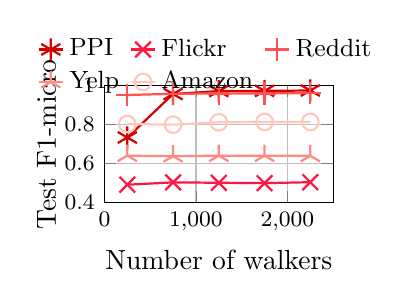
\begin{tikzpicture}
\def \ppi{asterisk}
\def \flickr{x}
\def \reddit{+}
\def \yelp{Mercedes star}
\def \amazon{o}
\begin{axis}[grid,xmin=0,xmax=2500,ymin=0.4,ymax=1,
    ylabel={Test F1-micro},
    xlabel={Number of walkers},
 %   xlabel shift=-15 pt,
    width=\plotwidth,
    height=\plotheight,
    tick label style={font=\footnotesize},
    y label style={at={(axis description cs:-0.17,.5)},anchor=south},
    scatter/classes={%
    ppi={mark=\ppi,red},
    flickr={mark=\flickr,black!70,thick},
    reddit={mark=\reddit,black!70,thick},
    yelp={mark=\yelp,black!70,thick}},
    legend style={font=\small},
    legend cell align=left,
    legend columns=3,
    legend style={at={(0.45,1.5)},anchor=north,/tikz/column 4/.style={column sep=5pt},draw=none,fill=none,/tikz/every even column/.append style={column sep=0.07cm}}
]

\addplot[thick,color=c1,mark=\ppi] 
    coordinates{(250,0.734)(750,0.957)(1250,0.972)(1750,0.973)(2250,0.975)};
\addplot[thick,color=c2,mark=\flickr]
    coordinates{(250,0.492)(750,0.504)(1250,0.502)(1750,0.500)(2250,0.505)};
\addplot[thick,color=c3,mark=\reddit]
    coordinates{(250,0.952)(750,0.958)(1250,0.960)(1750,0.960)(2250,0.962)};
\addplot[thick,color=c4,mark=\yelp]
    coordinates{(250,0.641)(750,0.638)(1250,0.641)(1750,0.641)(2250,0.640)};
\addplot[thick,color=c5,mark=\amazon,mark size=3pt]
    coordinates{(250,0.803)(750,0.800)(1250,0.812)(1750,0.814)(2250,0.814)};
    
\legend{PPI,Flickr,Reddit,Yelp,Amazon}
\end{axis}


\end{tikzpicture}}
% \hfill
% \subcaptionbox{Fraction of training time on sampling\label{fig: preproc cost}}[0.48\linewidth]{\definecolor{skyblue}{RGB}{213,0,0}
\definecolor{yellowgreen}{RGB}{255,23,68}
\definecolor{darkyellow}{RGB}{255,82,82}
\definecolor{orange}{RGB}{255,138,128}

\begin{tikzpicture}
\begin{axis}[
    enlarge x limits=0.2,ymin=0,ymax=1.8,
    ybar=\pgflinewidth,
    tick align=inside,
    xtick=data,
    x tick label style={rotate=90},
    bar width=5pt,
    ymajorgrids = true,
    symbolic x coords={PPI, Flickr, Reddit, Yelp, Amazon},
    ylabel=Fraction of training time,
    width=\textwidth,
    height=0.8\textwidth,
    y label style={at={(axis description cs:0.1,.6)},anchor=south},
    yticklabel style={/pgf/number format/precision=2,/pgf/number format/fixed},
    legend style={font=\small},
    legend cell align=left,
    legend columns=5,
    legend style={at={(0.5,1.2)},anchor=north,/tikz/column 5/.style={column sep=5pt},draw=none,/tikz/every even column/.append style={column sep=0.1cm}}]
\addplot[style={skyblue,fill=skyblue,mark=none}]
            coordinates {(PPI,.006) (Flickr,.012) (Reddit,0.205) (Yelp,.145) (Amazon, 0.506)};
\addplot[style={yellowgreen,fill=yellowgreen,mark=none}]
            coordinates {(PPI,0.053) (Flickr,0.114) (Reddit,0.178) (Yelp,.006)(Amazon,0.07)};  
\addplot[style={darkyellow,fill=darkyellow,mark=none}]
            coordinates {(PPI, .007) (Flickr,.232) (Reddit,.222) (Yelp,.08)(Amazon,0.116)};  
% \addplot[style={orange,fill=orange,mark=none}]
%             coordinates {(PPI, .08436/2) (Flickr,.24003/2) (Reddit,.13430/2) (Yelp,.25785/2)};  
\addplot[style={orange,fill=orange,mark=none}]
            coordinates {(PPI, .21) (Flickr,1.59) (Reddit,1.20) (Yelp,.747)(Amazon,0.970)};  
            
\legend{Node,Edge,RW,MRW}
\pgfplotsset{
    legend image code/.code={
        \draw [#1] (0cm,-0.1cm) rectangle (0.4cm,0.1cm);
    },
}
\end{axis}
\fill [white] (0.1,-0.5) rectangle (0.2,-1.44);%-0.5,-1.34
\end{tikzpicture}}
% \end{figure}



\paragraph{Evaluation on graph samplers} From Table \ref{tab: exp-sota}, random edge and random walk based samplers achieve higher accuracy than the random node sampler. Figure \ref{fig: sensitivity} presents sensitivity analysis on parameters of ``RW''. We use the same hyperparameters (except the sampling parameters) and network architecture as those of the ``RW'' entries in  Table \ref{tab: exp-sota}. We fix the length of each walker to $2$ (i.e., GCN depth), and vary the number of roots $r$ from $250$ to $2250$. For PPI, increasing $r$ from $250$ to $750$ significantly improves accuracy. Overall, for all datasets, accuracy stabilizes beyond $r=750$. 

% \subsection{Evaluation on Pre-Processing and Sampling Cost}
% \label{sec: exp-preproc}


%Note that the baselines also require pre-processing. 
%For the case of S-GCN, the time to pre-compute the first layer aggregation and setup data structures is equivalent to a\% to b\% of its training time. 


%\paragraph{Pre-processing cost} 
% describe how many samplers needed for estimating probability. Point out that for PPI and Yelp, pre-processing cost is 0. For Flickr and Reddit, pre-processing is another 10\% of training time. Pre-processing cost of other methods is significant. 


\subsection{{\graphsaint} on Architecture Variants and Deep Models\label{sec: exp extension}}



% \begin{figure}
% 	\begin{subfigure}[b]{0.66\textwidth}		
%     \begin{tikzpicture}

\def\plotwidth{0.37\textwidth}
\def\plotheight{.253\textwidth}%.2

\definecolor{gcnc}{RGB}{199,21,133}
\definecolor{gsagec}{RGB}{106,90,205}
\definecolor{fastgcnc}{RGB}{218,165,32}
\definecolor{sgcnc}{RGB}{139,69,19}
\definecolor{asgcnc}{RGB}{34,139,34}
\definecolor{cgcnc}{RGB}{0,139,139}
\definecolor{gsaintc}{RGB}{255,0,0}

\definecolor{c1}{RGB}{213,0,0}
\definecolor{c2}{RGB}{255,23,68}
\definecolor{c3}{RGB}{255,82,82}
\definecolor{c4}{RGB}{255,138,128}
\definecolor{b1}{RGB}{0,0,213}
\definecolor{b2}{RGB}{68,23,255}
\definecolor{b3}{RGB}{82,82,255}
\definecolor{b4}{RGB}{135,206,255}

\begin{groupplot}[
    group style={
    group size=2 by 1,
    y descriptions at=edge left,
    horizontal sep=3mm},
    scale only axis,
    %ymin=.945,ymax=.975,
    %ylabel shift=-40pt,
    xmode=log,
    height=\plotheight,
    tick label style={font=\footnotesize},
    title style={font=\small,at={(axis description cs:0.5, 0.95)}},
    grid,
    xmin=1E0,xmax=3E4,ymin=.925,ymax=.975,
    ylabel={Validation F1-micro},
    y label style={at={(axis description cs:0.15,.5)},anchor=south},
    /tikz/line join=round,
    ytick={0.93,0.94,0.95,0.96,0.97},
    %yticklabels={0.2,0.4,0.6,0.8,1},
    % every axis y label/.style={rotate=90,
    % at={(ticklabel* cs:1.05)},anchor=center,
    % },
    %ylabel shift=-40pt,
]

%%%%%%%%%%%%%%%%%%%%%%%%%%%%%%%%%%%
\nextgroupplot[
    title={\small GAT},
    every axis title/.style={below left,at={(1.,1)}},
    width=\plotwidth,
    %xmin=0,xmax=60,
    %ylabel={\small Validation F1-micro},
    %every axis y label/.append style={at=(ticklabel cs:-0.3)},
    %ylabel shift=-40 pt,
    xlabel={Training time (second)},
    every axis x label/.append style={at=(ticklabel cs:1.0)},
    xlabel shift=-17pt,
]
\addplot[color=c4,line width=0.8pt,/tikz/line join=round] coordinates{
(14.05,0.7471)
(16.49,0.8935)
(18.88,0.9273)
(21.15,0.9476)
(23.35,0.9531)
(25.79,0.9557)
(27.97,0.9584)
(30.29,0.9610)
(32.60,0.9610)
(35.05,0.9615)
(37.48,0.9615)
(39.93,0.9625)
(42.44,0.9617)
(44.70,0.9634)
(47.24,0.9627)
(49.54,0.9633)
(51.91,0.9638)
(54.25,0.9649)
(56.58,0.9642)
(58.86,0.9654)
(61.22,0.9646)
(63.76,0.9646)
(66.07,0.9641)
(68.47,0.9651)
(70.82,0.9656)
(73.23,0.9655)
(75.82,0.9648)
(78.26,0.9660)
(80.53,0.9655)
(82.84,0.9654)
(85.43,0.9663)
(87.73,0.9664)
(90.30,0.9670)
(92.73,0.9672)
(94.92,0.9664)
(97.46,0.9658)
(99.87,0.9670)
(102.36,0.9664)
(105.00,0.9659)
(107.75,0.9657)
};
\addplot[color=c1,line width=0.8pt,/tikz/line join=round]
coordinates{
(30.53,0.4927)
(34.01,0.5818)
(37.79,0.6796)
(41.51,0.7622)
(45.11,0.7851)
(48.76,0.8257)
(52.43,0.8723)
(56.11,0.8844)
(59.59,0.9208)
(63.03,0.9155)
(66.56,0.9370)
(69.96,0.9421)
(73.42,0.9446)
(77.05,0.9474)
(80.53,0.9457)
(84.19,0.9521)
(87.66,0.9539)
(91.07,0.9510)
(94.64,0.9500)
(98.18,0.9552)
(101.69,0.9568)
(105.17,0.9526)
(108.68,0.9565)
(112.27,0.9563)
(115.75,0.9603)
(119.37,0.9576)
(123.00,0.9584)
(126.66,0.9553)
(130.37,0.9604)
(133.93,0.9589)
(137.48,0.9592)
(141.10,0.9608)
(144.65,0.9612)
(148.38,0.9603)
(152.20,0.9618)
(156.12,0.9623)
(160.10,0.9620)
(164.12,0.9613)
(167.94,0.9601)
(171.86,0.9624)
(175.67,0.9611)
(179.52,0.9621)
(183.40,0.9598)
(187.25,0.9634)
(191.19,0.9613)
(195.05,0.9622)
(198.99,0.9631)
(202.76,0.9628)
(206.78,0.9612)
(210.73,0.9623)
(214.36,0.9615)
};
\addplot[color=b4,line width=0.8pt,/tikz/line join=round] coordinates{(1e-9,0.0)(40.66227,0.94814)(78.96042,0.95042)(116.46261,0.95131)(153.55791,0.95299)(190.41264,0.95227)(227.09808,0.95226)(263.65878,0.95506)(300.12444,0.95343)(336.52476,0.9526)(372.86568,0.95278)};
\addplot[color=b1,line width=0.8pt,/tikz/line join=round]
coordinates{(1e-9,0.0)(1010.25969,0.14688)(2008.0031399999998,0.14688)(2997.35502,0.29402)(3981.39698,0.7232)(4962.30988,0.87257)(5941.13674,0.89611)(6929.68265,0.91152)(7915.71583,0.91662)(8902.83944,0.92367)(9898.307209999999,0.92219)(10902.688059999999,0.92827)(11908.017109999999,0.92649)(12922.49629,0.93029)(13945.177399999999,0.92882)(14972.883969999999,0.9305)(16004.85744,0.93021)(17043.65795,0.93017)(18089.901830000003,0.93282)(19136.477580000002,0.92645)(20183.14815,0.92928)};

%%%%%%%%%%%%%%%%%%%%%%%%%%%%%%%%%%
\nextgroupplot[
    title={\small JK-net},
    every axis title/.style={below left,at={(1,1)}},
    width=\plotwidth,
    %xmin=0,xmax=40,
    legend cell align=left,
    legend columns=2,
    legend style={at={(-0.,1.52),font=\footnotesize},anchor=north,/tikz/column 2/.style={column sep=5pt},draw=none},
    ]
\addplot[thick,color=c4]coordinates{(3.6531,0.755306)
(3.9305,0.839613)
(4.2179,0.901515)
(4.4998,0.931811)
(4.7849,0.946538)
(5.0595,0.955694)
(5.3381,0.958606)
(5.6187,0.959365)
(5.9115,0.961728)
(6.2178,0.961855)
(6.5138,0.962446)
(6.7933,0.961855)
(7.0692,0.963290)
(7.3436,0.962572)
(7.6599,0.965737)
(7.9359,0.964429)
(8.2213,0.965062)
(8.5159,0.963880)
(8.8011,0.965526)
(9.0818,0.965357)
(9.3921,0.964851)
(9.6705,0.964007)
(9.9462,0.965442)
(10.2265,0.965568)
(10.5290,0.966201)
(10.8093,0.965821)
(11.0871,0.965948)
(11.3651,0.966285)
(11.6463,0.966243)
(11.9249,0.966285)
(12.1994,0.965610)
(12.4873,0.965020)
(12.7654,0.964176)
(13.0567,0.965104)
(13.3421,0.965231)
(13.6249,0.965990)
(13.9126,0.966328)
(14.2278,0.965610)
(14.5042,0.965231)};
\addplot[thick,color=c1] coordinates{(4.7239,0.600616)
(5.2210,0.679227)
(5.6767,0.727330)
(6.1452,0.787291)
(6.6077,0.835774)
(7.0685,0.871387)
(7.5297,0.912781)
(7.9955,0.911853)
(8.4841,0.928436)
(8.9468,0.945736)
(9.4079,0.952276)
(9.8740,0.955441)
(10.3384,0.956918)
(10.8111,0.960167)
(11.2713,0.960800)
(11.7272,0.962488)
(12.2000,0.962994)
(12.6611,0.963712)
(13.1301,0.963627)
(13.5970,0.965188)
(14.0549,0.965695)
(14.5243,0.966539)
(14.9923,0.965568)
(15.4596,0.965104)
(15.9287,0.967172)
(16.3993,0.966370)
(16.8616,0.967551)
(17.3259,0.967256)
(17.7876,0.966834)
(18.2497,0.967931)
(18.7242,0.967973)
(19.1884,0.967425)
(19.6509,0.968606)
(20.1089,0.967340)
(20.5688,0.967509)
(21.0255,0.967720)
(21.4880,0.967256)
(21.9445,0.968395)
(22.4047,0.968395)
(22.8836,0.968142)
(23.3417,0.968227)
(23.8015,0.969155)
(24.2661,0.969028)
(24.7366,0.968564)
(25.1947,0.969155)
(25.6595,0.968269)
(26.1257,0.967720)
(26.5882,0.969155)
(27.0482,0.968606)
(27.5124,0.969281)
(27.9685,0.969619)
(28.4386,0.967805)
(28.8937,0.967762)
(29.3694,0.967931)
(29.8314,0.969028)
(30.2923,0.969450)
(30.7516,0.968859)
(31.2092,0.968775)
(31.6729,0.968269)
(32.1350,0.969239)
(32.6020,0.969619)
(33.0610,0.970210)
(33.5169,0.969577)
(33.9748,0.970125)
(34.4405,0.969155)};
\addplot[thick,color=b4]coordinates{(11,0.31094)
(18,0.95312)
(25,0.952)
(32,0.95312)
(40,0.95794)
(47,0.94931)
(54,0.94731)
(61,0.94922)
(68,0.95312)
(75,0.9636)
(82,0.95903)
(89,0.95359)
(96,0.95569)
(103,0.94578)
(110,0.94188)
(118,0.94531)
(126,0.94922)
(132,0.95312)
(140,0.92969)};
\addplot[thick,color=b1] coordinates{(106.78,0.20703)
(209,0.91016)
(312,0.93750)
(415,0.92758)
(518,0.93750)
(622,0.93359)
(725,0.94531)
(829,0.95312)
(932,0.94531)
(1035,0.963)
(1138,0.94922)
(1241,0.95312)
(1344,0.95703)
(1448,0.93359)
(1551,0.93750)};


% \nextgroupplot[group/empty plot]

\legend{{\graphsaint} 2-layer, {\graphsaint} 4-layer, GraphSAGE 2-layer, GraphSAGE 4-layer}

%%%%%%%%%%%%%%%%%%%%%%%%%%%%%%%%%%

\end{groupplot}

\end{tikzpicture}

% 	\caption{Expressed as Hadamard}
% 	\label{fig: tilingA}
% 	\end{subfigure}
% 	\begin{subfigure}[b]{0.33\textwidth}
% 	\begin{tikzpicture}

\def\plotwidth{0.37\textwidth}
\def\plotheight{.253\textwidth}%.2

\definecolor{gcnc}{RGB}{199,21,133}
\definecolor{gsagec}{RGB}{106,90,205}
\definecolor{fastgcnc}{RGB}{218,165,32}
\definecolor{sgcnc}{RGB}{139,69,19}
\definecolor{asgcnc}{RGB}{34,139,34}
\definecolor{cgcnc}{RGB}{0,139,139}
\definecolor{gsaintc}{RGB}{255,0,0}

\definecolor{c1}{RGB}{213,0,0}
\definecolor{c2}{RGB}{255,23,68}
\definecolor{c3}{RGB}{255,82,82}
\definecolor{c4}{RGB}{255,138,128}
\definecolor{b1}{RGB}{0,0,213}
\definecolor{b2}{RGB}{68,23,255}
\definecolor{b3}{RGB}{82,82,255}
\definecolor{b4}{RGB}{135,206,255}

\begin{groupplot}[
    group style={
    group size=2 by 1,
    y descriptions at=edge left,
    horizontal sep=3mm},
    scale only axis,
    %ymin=.945,ymax=.975,
    %ylabel shift=-40pt,
    xmode=log,
    height=\plotheight,
    tick label style={font=\footnotesize},
    title style={font=\small,at={(axis description cs:0.5, 0.95)}},
    grid,
    xmin=1E0,xmax=3E4,ymin=.925,ymax=.975,
    ylabel={Validation F1-micro},
    y label style={at={(axis description cs:0.15,.5)},anchor=south},
    /tikz/line join=round,
    ytick={0.93,0.94,0.95,0.96,0.97},
    %yticklabels={0.2,0.4,0.6,0.8,1},
    % every axis y label/.style={rotate=90,
    % at={(ticklabel* cs:1.05)},anchor=center,
    % },
    %ylabel shift=-40pt,
]

%%%%%%%%%%%%%%%%%%%%%%%%%%%%%%%%%%%
\nextgroupplot[
    title={\small GAT},
    every axis title/.style={below left,at={(1.,1)}},
    width=\plotwidth,
    %xmin=0,xmax=60,
    %ylabel={\small Validation F1-micro},
    %every axis y label/.append style={at=(ticklabel cs:-0.3)},
    %ylabel shift=-40 pt,
    xlabel={Training time (second)},
    every axis x label/.append style={at=(ticklabel cs:1.0)},
    xlabel shift=-17pt,
]
\addplot[color=c4,line width=0.8pt,/tikz/line join=round] coordinates{
(14.05,0.7471)
(16.49,0.8935)
(18.88,0.9273)
(21.15,0.9476)
(23.35,0.9531)
(25.79,0.9557)
(27.97,0.9584)
(30.29,0.9610)
(32.60,0.9610)
(35.05,0.9615)
(37.48,0.9615)
(39.93,0.9625)
(42.44,0.9617)
(44.70,0.9634)
(47.24,0.9627)
(49.54,0.9633)
(51.91,0.9638)
(54.25,0.9649)
(56.58,0.9642)
(58.86,0.9654)
(61.22,0.9646)
(63.76,0.9646)
(66.07,0.9641)
(68.47,0.9651)
(70.82,0.9656)
(73.23,0.9655)
(75.82,0.9648)
(78.26,0.9660)
(80.53,0.9655)
(82.84,0.9654)
(85.43,0.9663)
(87.73,0.9664)
(90.30,0.9670)
(92.73,0.9672)
(94.92,0.9664)
(97.46,0.9658)
(99.87,0.9670)
(102.36,0.9664)
(105.00,0.9659)
(107.75,0.9657)
};
\addplot[color=c1,line width=0.8pt,/tikz/line join=round]
coordinates{
(30.53,0.4927)
(34.01,0.5818)
(37.79,0.6796)
(41.51,0.7622)
(45.11,0.7851)
(48.76,0.8257)
(52.43,0.8723)
(56.11,0.8844)
(59.59,0.9208)
(63.03,0.9155)
(66.56,0.9370)
(69.96,0.9421)
(73.42,0.9446)
(77.05,0.9474)
(80.53,0.9457)
(84.19,0.9521)
(87.66,0.9539)
(91.07,0.9510)
(94.64,0.9500)
(98.18,0.9552)
(101.69,0.9568)
(105.17,0.9526)
(108.68,0.9565)
(112.27,0.9563)
(115.75,0.9603)
(119.37,0.9576)
(123.00,0.9584)
(126.66,0.9553)
(130.37,0.9604)
(133.93,0.9589)
(137.48,0.9592)
(141.10,0.9608)
(144.65,0.9612)
(148.38,0.9603)
(152.20,0.9618)
(156.12,0.9623)
(160.10,0.9620)
(164.12,0.9613)
(167.94,0.9601)
(171.86,0.9624)
(175.67,0.9611)
(179.52,0.9621)
(183.40,0.9598)
(187.25,0.9634)
(191.19,0.9613)
(195.05,0.9622)
(198.99,0.9631)
(202.76,0.9628)
(206.78,0.9612)
(210.73,0.9623)
(214.36,0.9615)
};
\addplot[color=b4,line width=0.8pt,/tikz/line join=round] coordinates{(1e-9,0.0)(40.66227,0.94814)(78.96042,0.95042)(116.46261,0.95131)(153.55791,0.95299)(190.41264,0.95227)(227.09808,0.95226)(263.65878,0.95506)(300.12444,0.95343)(336.52476,0.9526)(372.86568,0.95278)};
\addplot[color=b1,line width=0.8pt,/tikz/line join=round]
coordinates{(1e-9,0.0)(1010.25969,0.14688)(2008.0031399999998,0.14688)(2997.35502,0.29402)(3981.39698,0.7232)(4962.30988,0.87257)(5941.13674,0.89611)(6929.68265,0.91152)(7915.71583,0.91662)(8902.83944,0.92367)(9898.307209999999,0.92219)(10902.688059999999,0.92827)(11908.017109999999,0.92649)(12922.49629,0.93029)(13945.177399999999,0.92882)(14972.883969999999,0.9305)(16004.85744,0.93021)(17043.65795,0.93017)(18089.901830000003,0.93282)(19136.477580000002,0.92645)(20183.14815,0.92928)};

%%%%%%%%%%%%%%%%%%%%%%%%%%%%%%%%%%
\nextgroupplot[
    title={\small JK-net},
    every axis title/.style={below left,at={(1,1)}},
    width=\plotwidth,
    %xmin=0,xmax=40,
    legend cell align=left,
    legend columns=2,
    legend style={at={(-0.,1.52),font=\footnotesize},anchor=north,/tikz/column 2/.style={column sep=5pt},draw=none},
    ]
\addplot[thick,color=c4]coordinates{(3.6531,0.755306)
(3.9305,0.839613)
(4.2179,0.901515)
(4.4998,0.931811)
(4.7849,0.946538)
(5.0595,0.955694)
(5.3381,0.958606)
(5.6187,0.959365)
(5.9115,0.961728)
(6.2178,0.961855)
(6.5138,0.962446)
(6.7933,0.961855)
(7.0692,0.963290)
(7.3436,0.962572)
(7.6599,0.965737)
(7.9359,0.964429)
(8.2213,0.965062)
(8.5159,0.963880)
(8.8011,0.965526)
(9.0818,0.965357)
(9.3921,0.964851)
(9.6705,0.964007)
(9.9462,0.965442)
(10.2265,0.965568)
(10.5290,0.966201)
(10.8093,0.965821)
(11.0871,0.965948)
(11.3651,0.966285)
(11.6463,0.966243)
(11.9249,0.966285)
(12.1994,0.965610)
(12.4873,0.965020)
(12.7654,0.964176)
(13.0567,0.965104)
(13.3421,0.965231)
(13.6249,0.965990)
(13.9126,0.966328)
(14.2278,0.965610)
(14.5042,0.965231)};
\addplot[thick,color=c1] coordinates{(4.7239,0.600616)
(5.2210,0.679227)
(5.6767,0.727330)
(6.1452,0.787291)
(6.6077,0.835774)
(7.0685,0.871387)
(7.5297,0.912781)
(7.9955,0.911853)
(8.4841,0.928436)
(8.9468,0.945736)
(9.4079,0.952276)
(9.8740,0.955441)
(10.3384,0.956918)
(10.8111,0.960167)
(11.2713,0.960800)
(11.7272,0.962488)
(12.2000,0.962994)
(12.6611,0.963712)
(13.1301,0.963627)
(13.5970,0.965188)
(14.0549,0.965695)
(14.5243,0.966539)
(14.9923,0.965568)
(15.4596,0.965104)
(15.9287,0.967172)
(16.3993,0.966370)
(16.8616,0.967551)
(17.3259,0.967256)
(17.7876,0.966834)
(18.2497,0.967931)
(18.7242,0.967973)
(19.1884,0.967425)
(19.6509,0.968606)
(20.1089,0.967340)
(20.5688,0.967509)
(21.0255,0.967720)
(21.4880,0.967256)
(21.9445,0.968395)
(22.4047,0.968395)
(22.8836,0.968142)
(23.3417,0.968227)
(23.8015,0.969155)
(24.2661,0.969028)
(24.7366,0.968564)
(25.1947,0.969155)
(25.6595,0.968269)
(26.1257,0.967720)
(26.5882,0.969155)
(27.0482,0.968606)
(27.5124,0.969281)
(27.9685,0.969619)
(28.4386,0.967805)
(28.8937,0.967762)
(29.3694,0.967931)
(29.8314,0.969028)
(30.2923,0.969450)
(30.7516,0.968859)
(31.2092,0.968775)
(31.6729,0.968269)
(32.1350,0.969239)
(32.6020,0.969619)
(33.0610,0.970210)
(33.5169,0.969577)
(33.9748,0.970125)
(34.4405,0.969155)};
\addplot[thick,color=b4]coordinates{(11,0.31094)
(18,0.95312)
(25,0.952)
(32,0.95312)
(40,0.95794)
(47,0.94931)
(54,0.94731)
(61,0.94922)
(68,0.95312)
(75,0.9636)
(82,0.95903)
(89,0.95359)
(96,0.95569)
(103,0.94578)
(110,0.94188)
(118,0.94531)
(126,0.94922)
(132,0.95312)
(140,0.92969)};
\addplot[thick,color=b1] coordinates{(106.78,0.20703)
(209,0.91016)
(312,0.93750)
(415,0.92758)
(518,0.93750)
(622,0.93359)
(725,0.94531)
(829,0.95312)
(932,0.94531)
(1035,0.963)
(1138,0.94922)
(1241,0.95312)
(1344,0.95703)
(1448,0.93359)
(1551,0.93750)};


% \nextgroupplot[group/empty plot]

\legend{{\graphsaint} 2-layer, {\graphsaint} 4-layer, GraphSAGE 2-layer, GraphSAGE 4-layer}

%%%%%%%%%%%%%%%%%%%%%%%%%%%%%%%%%%

\end{groupplot}

\end{tikzpicture}

% 	\caption{Expressed as dot product}
% 	\label{fig: tilingB}
% 	\end{subfigure}
% \vspace{-.4cm}
% \caption{Two views of spectral convolution of a layer}
% \label{fig: tiling}
% \vspace{-0.7cm}
% \end{figure}


\begin{figure}
    \centering
    \begin{minipage}{0.33\textwidth}
        \centering
        \tikzset{mark size=4}

\pgfplotsset{
compat=1.11,
legend image code/.code={
\draw[mark repeat=2,mark phase=2]
plot coordinates {
(0cm,0cm)
(0.15cm,0cm)        %% default is (0.3cm,0cm)
(0.3cm,0cm)         %% default is (0.6cm,0cm)
};%
}
}

\definecolor{c1}{RGB}{213,0,0}
\definecolor{c2}{RGB}{255,23,68}
\definecolor{c3}{RGB}{255,82,82}
\definecolor{c4}{RGB}{255,138,128}
\definecolor{c5}{RGB}{255,200,190}

\def\plotwidth{1.1\textwidth}
\def\plotheight{0.85\textwidth}%.75

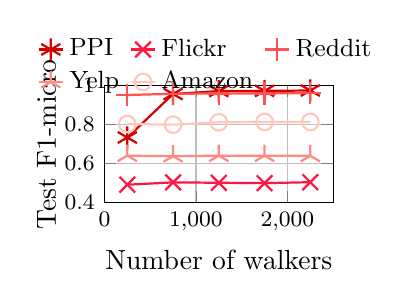
\begin{tikzpicture}
\def \ppi{asterisk}
\def \flickr{x}
\def \reddit{+}
\def \yelp{Mercedes star}
\def \amazon{o}
\begin{axis}[grid,xmin=0,xmax=2500,ymin=0.4,ymax=1,
    ylabel={Test F1-micro},
    xlabel={Number of walkers},
 %   xlabel shift=-15 pt,
    width=\plotwidth,
    height=\plotheight,
    tick label style={font=\footnotesize},
    y label style={at={(axis description cs:-0.17,.5)},anchor=south},
    scatter/classes={%
    ppi={mark=\ppi,red},
    flickr={mark=\flickr,black!70,thick},
    reddit={mark=\reddit,black!70,thick},
    yelp={mark=\yelp,black!70,thick}},
    legend style={font=\small},
    legend cell align=left,
    legend columns=3,
    legend style={at={(0.45,1.5)},anchor=north,/tikz/column 4/.style={column sep=5pt},draw=none,fill=none,/tikz/every even column/.append style={column sep=0.07cm}}
]

\addplot[thick,color=c1,mark=\ppi] 
    coordinates{(250,0.734)(750,0.957)(1250,0.972)(1750,0.973)(2250,0.975)};
\addplot[thick,color=c2,mark=\flickr]
    coordinates{(250,0.492)(750,0.504)(1250,0.502)(1750,0.500)(2250,0.505)};
\addplot[thick,color=c3,mark=\reddit]
    coordinates{(250,0.952)(750,0.958)(1250,0.960)(1750,0.960)(2250,0.962)};
\addplot[thick,color=c4,mark=\yelp]
    coordinates{(250,0.641)(750,0.638)(1250,0.641)(1750,0.641)(2250,0.640)};
\addplot[thick,color=c5,mark=\amazon,mark size=3pt]
    coordinates{(250,0.803)(750,0.800)(1250,0.812)(1750,0.814)(2250,0.814)};
    
\legend{PPI,Flickr,Reddit,Yelp,Amazon}
\end{axis}


\end{tikzpicture}
        \vspace{-.5cm}
        \captionof{figure}{Sensitivity analysis}
        \label{fig: sensitivity}
    \end{minipage}
    \begin{minipage}{0.66\textwidth}
        \centering
        \begin{tikzpicture}

\def\plotwidth{0.37\textwidth}
\def\plotheight{.253\textwidth}%.2

\definecolor{gcnc}{RGB}{199,21,133}
\definecolor{gsagec}{RGB}{106,90,205}
\definecolor{fastgcnc}{RGB}{218,165,32}
\definecolor{sgcnc}{RGB}{139,69,19}
\definecolor{asgcnc}{RGB}{34,139,34}
\definecolor{cgcnc}{RGB}{0,139,139}
\definecolor{gsaintc}{RGB}{255,0,0}

\definecolor{c1}{RGB}{213,0,0}
\definecolor{c2}{RGB}{255,23,68}
\definecolor{c3}{RGB}{255,82,82}
\definecolor{c4}{RGB}{255,138,128}
\definecolor{b1}{RGB}{0,0,213}
\definecolor{b2}{RGB}{68,23,255}
\definecolor{b3}{RGB}{82,82,255}
\definecolor{b4}{RGB}{135,206,255}

\begin{groupplot}[
    group style={
    group size=2 by 1,
    y descriptions at=edge left,
    horizontal sep=3mm},
    scale only axis,
    %ymin=.945,ymax=.975,
    %ylabel shift=-40pt,
    xmode=log,
    height=\plotheight,
    tick label style={font=\footnotesize},
    title style={font=\small,at={(axis description cs:0.5, 0.95)}},
    grid,
    xmin=1E0,xmax=3E4,ymin=.925,ymax=.975,
    ylabel={Validation F1-micro},
    y label style={at={(axis description cs:0.15,.5)},anchor=south},
    /tikz/line join=round,
    ytick={0.93,0.94,0.95,0.96,0.97},
    %yticklabels={0.2,0.4,0.6,0.8,1},
    % every axis y label/.style={rotate=90,
    % at={(ticklabel* cs:1.05)},anchor=center,
    % },
    %ylabel shift=-40pt,
]

%%%%%%%%%%%%%%%%%%%%%%%%%%%%%%%%%%%
\nextgroupplot[
    title={\small GAT},
    every axis title/.style={below left,at={(1.,1)}},
    width=\plotwidth,
    %xmin=0,xmax=60,
    %ylabel={\small Validation F1-micro},
    %every axis y label/.append style={at=(ticklabel cs:-0.3)},
    %ylabel shift=-40 pt,
    xlabel={Training time (second)},
    every axis x label/.append style={at=(ticklabel cs:1.0)},
    xlabel shift=-17pt,
]
\addplot[color=c4,line width=0.8pt,/tikz/line join=round] coordinates{
(14.05,0.7471)
(16.49,0.8935)
(18.88,0.9273)
(21.15,0.9476)
(23.35,0.9531)
(25.79,0.9557)
(27.97,0.9584)
(30.29,0.9610)
(32.60,0.9610)
(35.05,0.9615)
(37.48,0.9615)
(39.93,0.9625)
(42.44,0.9617)
(44.70,0.9634)
(47.24,0.9627)
(49.54,0.9633)
(51.91,0.9638)
(54.25,0.9649)
(56.58,0.9642)
(58.86,0.9654)
(61.22,0.9646)
(63.76,0.9646)
(66.07,0.9641)
(68.47,0.9651)
(70.82,0.9656)
(73.23,0.9655)
(75.82,0.9648)
(78.26,0.9660)
(80.53,0.9655)
(82.84,0.9654)
(85.43,0.9663)
(87.73,0.9664)
(90.30,0.9670)
(92.73,0.9672)
(94.92,0.9664)
(97.46,0.9658)
(99.87,0.9670)
(102.36,0.9664)
(105.00,0.9659)
(107.75,0.9657)
};
\addplot[color=c1,line width=0.8pt,/tikz/line join=round]
coordinates{
(30.53,0.4927)
(34.01,0.5818)
(37.79,0.6796)
(41.51,0.7622)
(45.11,0.7851)
(48.76,0.8257)
(52.43,0.8723)
(56.11,0.8844)
(59.59,0.9208)
(63.03,0.9155)
(66.56,0.9370)
(69.96,0.9421)
(73.42,0.9446)
(77.05,0.9474)
(80.53,0.9457)
(84.19,0.9521)
(87.66,0.9539)
(91.07,0.9510)
(94.64,0.9500)
(98.18,0.9552)
(101.69,0.9568)
(105.17,0.9526)
(108.68,0.9565)
(112.27,0.9563)
(115.75,0.9603)
(119.37,0.9576)
(123.00,0.9584)
(126.66,0.9553)
(130.37,0.9604)
(133.93,0.9589)
(137.48,0.9592)
(141.10,0.9608)
(144.65,0.9612)
(148.38,0.9603)
(152.20,0.9618)
(156.12,0.9623)
(160.10,0.9620)
(164.12,0.9613)
(167.94,0.9601)
(171.86,0.9624)
(175.67,0.9611)
(179.52,0.9621)
(183.40,0.9598)
(187.25,0.9634)
(191.19,0.9613)
(195.05,0.9622)
(198.99,0.9631)
(202.76,0.9628)
(206.78,0.9612)
(210.73,0.9623)
(214.36,0.9615)
};
\addplot[color=b4,line width=0.8pt,/tikz/line join=round] coordinates{(1e-9,0.0)(40.66227,0.94814)(78.96042,0.95042)(116.46261,0.95131)(153.55791,0.95299)(190.41264,0.95227)(227.09808,0.95226)(263.65878,0.95506)(300.12444,0.95343)(336.52476,0.9526)(372.86568,0.95278)};
\addplot[color=b1,line width=0.8pt,/tikz/line join=round]
coordinates{(1e-9,0.0)(1010.25969,0.14688)(2008.0031399999998,0.14688)(2997.35502,0.29402)(3981.39698,0.7232)(4962.30988,0.87257)(5941.13674,0.89611)(6929.68265,0.91152)(7915.71583,0.91662)(8902.83944,0.92367)(9898.307209999999,0.92219)(10902.688059999999,0.92827)(11908.017109999999,0.92649)(12922.49629,0.93029)(13945.177399999999,0.92882)(14972.883969999999,0.9305)(16004.85744,0.93021)(17043.65795,0.93017)(18089.901830000003,0.93282)(19136.477580000002,0.92645)(20183.14815,0.92928)};

%%%%%%%%%%%%%%%%%%%%%%%%%%%%%%%%%%
\nextgroupplot[
    title={\small JK-net},
    every axis title/.style={below left,at={(1,1)}},
    width=\plotwidth,
    %xmin=0,xmax=40,
    legend cell align=left,
    legend columns=2,
    legend style={at={(-0.,1.52),font=\footnotesize},anchor=north,/tikz/column 2/.style={column sep=5pt},draw=none},
    ]
\addplot[thick,color=c4]coordinates{(3.6531,0.755306)
(3.9305,0.839613)
(4.2179,0.901515)
(4.4998,0.931811)
(4.7849,0.946538)
(5.0595,0.955694)
(5.3381,0.958606)
(5.6187,0.959365)
(5.9115,0.961728)
(6.2178,0.961855)
(6.5138,0.962446)
(6.7933,0.961855)
(7.0692,0.963290)
(7.3436,0.962572)
(7.6599,0.965737)
(7.9359,0.964429)
(8.2213,0.965062)
(8.5159,0.963880)
(8.8011,0.965526)
(9.0818,0.965357)
(9.3921,0.964851)
(9.6705,0.964007)
(9.9462,0.965442)
(10.2265,0.965568)
(10.5290,0.966201)
(10.8093,0.965821)
(11.0871,0.965948)
(11.3651,0.966285)
(11.6463,0.966243)
(11.9249,0.966285)
(12.1994,0.965610)
(12.4873,0.965020)
(12.7654,0.964176)
(13.0567,0.965104)
(13.3421,0.965231)
(13.6249,0.965990)
(13.9126,0.966328)
(14.2278,0.965610)
(14.5042,0.965231)};
\addplot[thick,color=c1] coordinates{(4.7239,0.600616)
(5.2210,0.679227)
(5.6767,0.727330)
(6.1452,0.787291)
(6.6077,0.835774)
(7.0685,0.871387)
(7.5297,0.912781)
(7.9955,0.911853)
(8.4841,0.928436)
(8.9468,0.945736)
(9.4079,0.952276)
(9.8740,0.955441)
(10.3384,0.956918)
(10.8111,0.960167)
(11.2713,0.960800)
(11.7272,0.962488)
(12.2000,0.962994)
(12.6611,0.963712)
(13.1301,0.963627)
(13.5970,0.965188)
(14.0549,0.965695)
(14.5243,0.966539)
(14.9923,0.965568)
(15.4596,0.965104)
(15.9287,0.967172)
(16.3993,0.966370)
(16.8616,0.967551)
(17.3259,0.967256)
(17.7876,0.966834)
(18.2497,0.967931)
(18.7242,0.967973)
(19.1884,0.967425)
(19.6509,0.968606)
(20.1089,0.967340)
(20.5688,0.967509)
(21.0255,0.967720)
(21.4880,0.967256)
(21.9445,0.968395)
(22.4047,0.968395)
(22.8836,0.968142)
(23.3417,0.968227)
(23.8015,0.969155)
(24.2661,0.969028)
(24.7366,0.968564)
(25.1947,0.969155)
(25.6595,0.968269)
(26.1257,0.967720)
(26.5882,0.969155)
(27.0482,0.968606)
(27.5124,0.969281)
(27.9685,0.969619)
(28.4386,0.967805)
(28.8937,0.967762)
(29.3694,0.967931)
(29.8314,0.969028)
(30.2923,0.969450)
(30.7516,0.968859)
(31.2092,0.968775)
(31.6729,0.968269)
(32.1350,0.969239)
(32.6020,0.969619)
(33.0610,0.970210)
(33.5169,0.969577)
(33.9748,0.970125)
(34.4405,0.969155)};
\addplot[thick,color=b4]coordinates{(11,0.31094)
(18,0.95312)
(25,0.952)
(32,0.95312)
(40,0.95794)
(47,0.94931)
(54,0.94731)
(61,0.94922)
(68,0.95312)
(75,0.9636)
(82,0.95903)
(89,0.95359)
(96,0.95569)
(103,0.94578)
(110,0.94188)
(118,0.94531)
(126,0.94922)
(132,0.95312)
(140,0.92969)};
\addplot[thick,color=b1] coordinates{(106.78,0.20703)
(209,0.91016)
(312,0.93750)
(415,0.92758)
(518,0.93750)
(622,0.93359)
(725,0.94531)
(829,0.95312)
(932,0.94531)
(1035,0.963)
(1138,0.94922)
(1241,0.95312)
(1344,0.95703)
(1448,0.93359)
(1551,0.93750)};


% \nextgroupplot[group/empty plot]

\legend{{\graphsaint} 2-layer, {\graphsaint} 4-layer, GraphSAGE 2-layer, GraphSAGE 4-layer}

%%%%%%%%%%%%%%%%%%%%%%%%%%%%%%%%%%

\end{groupplot}

\end{tikzpicture}

        \vspace{-.13cm}
        \captionof{figure}{{\graphsaint} with JK-net and GAT (Reddit)}
        \label{fig: jk-gat-saint}
    \end{minipage}
\end{figure}



%As discussed in Section \ref{sec: discussion}, {\graphsaint} can be integrated into other GCN architecture variants. 
In Figure \ref{fig: jk-gat-saint}, we train a 2-layer and a 4-layer model of GAT \citep{gat} and JK-net \citep{jk-net}, by using minibatches of GraphSAGE and {\graphsaint} respectively. 
On the two 4-layer architectures, {\graphsaint} achieves two orders of magnitude speedup than GraphSAGE, indicating much better scalability on deep models. 
From accuracy perspective, 4-layer GAT-SAGE and JK-SAGE do not outperform the corresponding 2-layer versions, potentially due to the smoothening effect caused by the massive neighborhood size. On the other hand, with minibatches returned by our edge sampler, increasing model depth of JK-{\saint} leads to noticeable accuracy improvement (from 0.966 of 2-layer to 0.970 of 4-layer). 
Appendix \ref{appendix: depth} contains additional scalability results. 

% We integrate the jumping knowledge network (JK-Net) \cite{jk-net} into the {\graphsaint} framework, and evaluate the performance of a deep JK-Net trained by minibatches of subgraphs. 
% Figure \ref{fig: exp jk} shows the convergence curves of a 2-layer GCN (defined by Equation \ref{eq: vanilla gcn}; hidden dimension $128$) and a 4-layer JK-Net (defined in Appendix \ref{appendix: config}; hidden dimension $128$), both trained under the edge sampler. 
% The 2-layer GCN achieves $0.966$ F1-micro score, while the 4-layer JK-Net achieves over $0.970$ F1-micro score.
% Notably, the training time of the 4-layer model is only around twice that of the 2-layer model. 
% Under the setting of the original JK-Net paper \cite{jk-net}, the minibatch training uses the neighbor sampling of GraphSAGE \cite{graphsage}, and achieves $0.965$ F1-micro for a 2-layer model (hidden dimension $128$). However, such training of \cite{jk-net} can not scale to deeper networks. 
% The above results demonstrate that training based on the sampling of {\graphsaint} can be applied to other GCN architecture variants, to greatly improve their training efficiency without compromising accuracy.  